\documentclass[whitelogo]{TUD-report2020}

\usepackage[style=apa]{biblatex}
\usepackage{multirow}
\addbibresource{report.bib}
\usepackage{subcaption} 
\usepackage{graphicx}
\usepackage{minted}
\usepackage{enumitem}
\usepackage{csquotes}
\usepackage{longtable}

\usepackage{changes}
\begin{document}

%% Use Roman numerals for the page numbers of the title pages and table of
%% contents.
\frontmatter


%% Uncomment following 16 lines for a cover with a picture on the lower half only
\title[tudelft-white]{
  {\fontsize{45pt}{42pt}\selectfont Improving Forecast Accuracy for Offshore Wind Turbine Installation}
  }
\subtitle[tudelft-black]{
  {\fontsize{20pt}{26pt}\selectfont{A research of Hybrid ARIMA–ANN, Bayesian Neural Networks, and LSTMs with Refit Interval Strategies}}
  }
\author[tudelft-black]{Maximilianus J.A. Crebolder meergenaamd Krijbolder}
\affiliation{Technische Universiteit Delft}
\coverimage{images/Title-Page-2.png}
\covertext[tudelft-white]{
    \textbf{Delft University of Technology \\
    \small Image Source \cite{Picture-Title-Page}} \\
    }
    \setpagecolor{tudelft-cyan}
\makecover[split]


%% Include an optional title page.
\begin{titlepage}


\begin{center}

%% Insert the TU Delft logo at the bottom of the page.

%% Print the title in cyan.
{\makeatletter
\largetitlestyle\fontsize{32}{94}\selectfont\@title
%\largetitlestyle\color{tudelft-cyan}\Huge\@title
\makeatother}

%% Print the optional subtitle in black.
{\makeatletter
\ifx\@subtitle\undefined\else
    \bigskip
   {\tudsffamily\fontsize{22}{32}\selectfont\@subtitle}    
    %\titlefont\titleshape\LARGE\@subtitle
\fi
\makeatother}

\bigskip
\bigskip

by
%door

\bigskip
\bigskip

%% Print the name of the author.
{\makeatletter
%\largetitlefont\Large\bfseries\@author
\largetitlestyle\fontsize{26}{26}\selectfont\@author
\makeatother}

\bigskip
\bigskip

Research Assignment
%ter verkrijging van de graad van Master of Science

at the Delft University of Technology,
%aan de Technische Universiteit Delft,


\vfill

\begin{tabular}{lll}
    Student number: & 4830512 \\
    Project duration: & \multicolumn{2}{l}{September 9, 2024 -- March 14, 2025} \\
    Supervisor: & Dr.\ X.\ Jiang, & TU Delft \\
\end{tabular}
%% Only include the following lines if confidentiality is applicable.

\bigskip
\bigskip

%\emph{Op dit verslag is geheimhouding van toepassing tot en met 31 december 2013.}

\bigskip
\bigskip

%\\[1cm]

%\centering{
\includegraphics{cover/logo_black}}


\end{center}

\begin{tikzpicture}[remember picture, overlay]
    \node at (current page.south)[anchor=south,inner sep=0pt]{
        
\includegraphics{cover/logo_black}
    };
\end{tikzpicture}

\end{titlepage}



\chapter*{Abstract}
\setheader{Abstract}

An efficient and smooth installation of offshore wind-turbines, is highly influenced by the weather conditions. Accurate forecasting of the key weather parameter, significant wave height, mean wave frequency and  wind speed, is needed to minimize delays. These delays occur when operational limits of the vessels are reached and so downtime occurs, eventually leading to increased project costs. This research compares three advanced forecasting techniques: A Hybrid ARIMA-ANN model, which combines linear and non-linear components, a Bayesian Neural Network with Mont Carlo dropout, to find a probabilistic distribution in the solutions, a Long Short-Term Memory model, for long-term dependencies. All models where trained with 8 years, 2001-2008, of hourly data and tested on 2 years of data, 2009-2010, from a North Sea site. During the testing phase the models where refitted and retrained every 5 days. The Hybrid ARIMA-ANN model was further investigated and the effect of different refit intervals is investigated with a range from 6 hours to 4 weeks.\\

\noindent The models are evaluated with the following evaluation metrics, Mean Squared Error, Mean Absolute Error, Root Mean Squared Error and $R^2$, these reveal that frequent refit intervals load to an increase in accuracy but demands higher computational capability. The Hybrid ARIMA-ANN is the best performing model of the three, where it is able to capture the fluctuations in the data and in the mean time keeps the metrics to a minimum. In operational terms selecting an appropriate model will be site and operation specific, but the Hybrid model with a short refit interval \leq 1-day can reduce downtime and eventually lead to a smoother operation. The models where constructed in MatLab and can be found in GitHub 


\tableofcontents

%\chapter*{List of Symbols}
\addcontentsline{toc}{chapter}{List of Symbols} % Adds the entry to the table of contents (optional)

\begin{tabbing}
Symbol \quad \= Description \\
$a_t$ \> White noise error term in ARIMA model \\
$B$ \> Backshift (lag) operator \\
$b$ \> Bias term in neural network node calculation and in LSTM \\
$b_i$ \> Bias term for the input gate in LSTM \\
$b_z$ \> Bias term for the candidate memory cell in LSTM \\
$b_f$ \> Bias term for the forget gate in LSTM \\
$b_o$ \> Bias term for the output gate in LSTM \\
$c_p$ \> Specific heat capacity (J/(kg·K)) \\
$C_f$ \> Final time norm matrix in singular vector calculation \\
$C_i$ \> Initial time norm matrix in singular vector calculation \\
$C_t$ \> Cell state at time $t$ in LSTM \\
$d$ \> Differencing order in ARIMA model \\
$\Delta w_{ij}$ \> Change in weight between neurons $i$ and $j$ in backpropagation \\
$D$ \> Observed data used in BNN \\
$e(t)$ \> Residual error between observed and ARIMA forecast values \\
$E$ \> Error or loss function (e.g., Mean Squared Error) \\
$f$ \> External forces (N) or activation function \\
$f(x)$ \> Activation function \\
$f_t$ \> Forget gate activation at time $t$ in LSTM \\
$h$ \> Forecast horizon in Holt-Winters method \\
$h_t$ \> Hidden state at time $t$ in LSTM \\
$k$ \> Number of complete seasonal cycles between $t$ and $t+h$ \\
$L_t$ \> Level component at time $t$ in Holt-Winters method \\
$m$ \> Seasonal period length \\
$M$ \> Tangent linear model operator in singular vector calculation \\
$N$ \> Number of ensemble members or data points \\
$p$ \> Pressure (Pa) \\
$p(w)$ \> Prior distribution of weights in BNN \\
$p(w|D)$ \> Posterior distribution of weights given data in BNN \\
$p(D|w)$ \> Likelihood of the data given weights in BNN \\
$p(D)$ \> Evidence or marginal likelihood in BNN \\
$p(\hat{y}|D)$ \> Predictive distribution of output given data in BNN \\
$Q$ \> Heat source (W/m²) \\
$R$ \> Specific gas constant (J/(kg·K)) \\
$S_t$ \> Seasonal component at time $t$ in Holt-Winters method \\
$tanh$ \> Activation function in LSTM \\
$T$ \> Temperature (K) \\
$T_t$ \> Trend component at time $t$ in Holt-Winters method \\
$u$ \> Singular vector in singular vector calculation \\
$v$ \> Velocity field (m/s) \\
$w$ \> Weights in Bayesian Neural Network \\
$w_i$ \> Weight assigned to input $i$ in neural network \\
$x_i$ \> Forecast from the $i$-th ensemble member or input data \\
$x_t$ \> Input data at time $t$ in LSTM \\
$y$ \> Output of a neural network node \\
$y_i$ \> Actual observed value at data point $i$ \\
$y_{\text{ARIMA}}(t)$ \> Forecasted linear component from ARIMA model \\
$y_{\text{ANN}}(t)$ \> Forecasted non-linear component from ANN model \\
$y_{\text{hybrid}}(t)$ \> Combined forecast from ARIMA and ANN models \\
$\hat{y}_i$ \> Predicted value at data point $i$ \\
$z_t$ \> Candidate memory cell at time $t$ in LSTM \\
$\nu$ \> Viscosity (Pa·s) \\
$\rho$ \> Density (kg/m³) \\
$\sigma$ \> Sigmoid activation function in LSTM \\
$\sigma^2$ \> Singular value in singular vector calculation \\
$\theta(B)$ \> Moving average operator polynomial in ARIMA model \\
$\theta_0$ \> Constant term in ARIMA model \\
$\theta_i$ \> Moving average coefficient for lag $i$ in ARIMA model \\
$\varphi(B)$ \> Generalized autoregressive operator in ARIMA model \\
$\Phi(B)$ \> Autoregressive operator polynomial in ARIMA model \\
$\Phi_i$ \> Autoregressive coefficient for lag $i$ in ARIMA model \\
$o_t$ \> Output gate activation at time $t$ in LSTM \\
$i_t$ \> Input gate activation at time $t$ in LSTM \\
\end{tabbing}


%% Use Arabic numerals for the page numbers of the chapters.
\mainmatter

\chapter{Introduction}

\section{Background}
The energy sector is undergoing significant change, with a decline in fossil fuel use and a rise in renewable energy sources such as solar, nuclear, hydro, and wind energy (\cite{IEA2024}). By 2023, renewable energy represented almost 15\% of total energy production (\cite{EnergyInstitute2024}). To achieve zero emissions by 2025, these renewable resource areas need to be increased significantly.

Wind energy utilises the kinetic energy of wind to generate electricity. As a clean and sustainable option, it is one of the fastest-growing segments of the global energy market. Recent advancements in wind turbine design and materials have enhanced energy capture efficiency and reduced the levelized cost of electricity (LCOE) for wind energy production (\cite{GWEC2024}; \cite{GWEC2024Offshore}). These improvements result from scaling up production, increasing turbine sizes, and lowering installation and maintenance costs.

Establishing both onshore and offshore wind farms is needed to diversify the energy mix and to meet climate goals (\cite{IEA2024}). Offshore wind energy is especially significant because these farms benefit from faster and more consistent wind patterns compared to onshore installations (\cite{GWEC2024Offshore}). This leads to higher capacity factors,  greater energy production potential, and reduced operational costs (\cite{GWEC2024}). In addition, offshore wind turbines generally face fewer space and noise restrictions, allowing larger installations with less impact on local communities.

The global offshore wind industry is entering a new phase of growth, marked by record installations and supportive policies that drive future development (\cite{GWEC2024}). In 2023, the offshore wind sector had an operational capacity of 75 GW, in 2028 this is forecasted to be tripled (\cite{GWEC2024Offshore}). This sector also generates jobs and boosts economic growth in coastal regions (\cite{GWEC2024}).

To realize the full potential of offshore wind energy, accurate weather forecasting is essential for effective planning and installation of wind turbines. Met-ocean conditions, such as significant wave height, mean wave frequency, and wind speed, greatly influence the feasibility and efficiency of offshore projects. The vessels used in the installation phase operate within specific weather windows, which consist of multiple parts: loading components onto the vessel, transporting them to the site, and assembling them at sea, as can be seen in Figure \ref{fig:installation_process}.

\begin{figure}[h!]
\centering
\begin{tikzpicture}[>=stealth, node distance=5cm, on grid]

\tikzstyle{phase} = [rectangle, rounded corners, draw=black, fill=blue!10, 
                     text centered, text width=3.5cm, minimum height=2cm]

\node[phase] (loading) {
  \textbf{Loading} \\
  \footnotesize Components loaded \\
  \footnotesize onto vessel \\
};

\node[phase, right=of loading] (transit) {
  \textbf{Transit} \\
  \footnotesize Vessel at sea \\
};

\node[phase, right=of transit] (assembly) {
  \textbf{Assembly} \\
  \footnotesize Turbine \\
  \footnotesize installation \\
};

\draw[->, thick] (loading) -- (transit);
\draw[->, thick] (transit) -- (assembly);

\end{tikzpicture}
\caption{Overview of the offshore wind turbine installation process}
\label{fig:installation_process}
\end{figure}

\newpage
These tasks are carried out by different vessels that will be limited by the met-ocean conditions. Using advanced forecasting methods, developers can better predict and manage installation timelines, ultimately reducing delays caused by adverse weather. Moreover, accurate forecasting can optimise wind turbine placement and design, ensuring that installations are tailored to local conditions for maximum output. This precision helps to achieve better project results and ensures safer offshore operations. From an economic standpoint, when delays occur, vessels must still be rented while no installation occurs, leading to increased costs.

Understanding and predicting met-ocean conditions will help to capture risks associated with installation and operation. So, enhancing the overall performance of wind energy systems. By integrating reliable forecasting into the planning stages, the offshore wind sector can make informed decisions. This will lead to less delays and so an overall more efficient installation process (\cite{IEA2021}; \cite{GWEC2024Offshore}).

\section{Problem Statement}
Offshore wind farms are an essential part of the transition towards renewable energy. However, ocean conditions often ground specialized installation vessels, along with their crews, as they wait for safe weather to load, transport and assemble wind turbine components at sea. These delays can quickly increase project costs and potentially damage equipment if wave conditions or wind speeds go above forecast thresholds (\cite{Boccaletti2019}; \cite{Kelley2018}).

Although the stakes are high, current forecasting methods fall short in two main areas. First, many techniques lack sufficient accuracy for dynamic offshore environments, where complex wave, wind, and atmospheric interactions are interdependent (\cite{Murphy1993}; \cite{Wilks2011}). Second, most models often cannot quickly adapt to local changes, leaving operators with inaccurate predictions during the installation windows. This makes it easy to underestimate a storm or miscalculate the frequency of wave activity, with the safety of crew and project schedules at risk.

In response, researchers started experimenting with more advanced models, ranging from hybrid and probabilistic approaches to deep learning techniques (\cite{Zhang2019}; \cite{Huang2020}). However, there remains a need to compare these methods side by side under realistic offshore scenarios and changing refit intervals. This comparison aims to determine which model best balances accuracy, reliability, and practicality.

 The research investigates three advanced forecasting strategies: a Bayesian Neural Network with Monte Carlo Dropout, an LSTM-based deep learning approach, and a Hybrid ARIMA–ANN model. Focusing on significant wave height, mean wave frequency, and wind speed. By evaluating how each parameter performs under real data conditions, this research aims to reduce weather-related project delays and streamline the installation of offshore wind turbines. The process is visualized in Figure \ref{fig:forecast_process}. The objective is to lower operational costs but also enhance safety for those working in the renewable energy sector. 

\begin{figure}[h!]
    \centering
    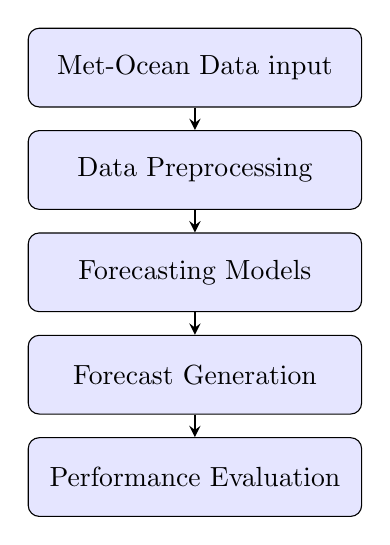
\begin{tikzpicture}[node distance=1.3 cm, auto]

    \tikzstyle{block} = [rectangle, draw, fill=blue!10, rounded corners, text width=4 cm, text centered, minimum height=1 cm]
    \tikzstyle{arrow} = [thick,->,>=stealth]
    
    \node[block] (data) {Met-Ocean Data input};
    \node[block, below of=data] (preprocessing) {Data Preprocessing};
    \node[block, below of=preprocessing] (models) {Forecasting Models};
    \node[block, below of=models] (forecast) {Forecast Generation};
    \node[block, below of=forecast] (evaluation) {Performance Evaluation};
    
    \draw[arrow] (data) -- (preprocessing);
    \draw[arrow] (preprocessing) -- (models);
    \draw[arrow] (models) -- (forecast);
    \draw[arrow] (forecast) -- (evaluation);
    
    \end{tikzpicture}
    \caption{Flow diagram of the forecasting process used in this research.}
    \label{fig:forecast_process}
\end{figure}

 
\section{Research Question and Sub-questions}
To effectively address the challenges associated with weather forecasting for offshore wind turbine installation, research questions are formulated. This study will investigate how various forecasting models can enhance the accuracy of weather predictions, thereby ensuring a more streamlined installation process. 

\subsection*{Research Question}  
How can weather forecasts for significant wave height, mean wave frequency, and wind speed be improved for offshore wind turbine installations by comparing hybrid, probabilistic, and deep learning models, and what is the impact of varying refit intervals on forecast performance?

\subsection*{Sub-questions}
\begin{enumerate}
    \item What are the strengths and limitations of hybrid, probabilistic, and deep learning models for forecasting key weather conditions in offshore wind turbine installation?
    \item How do the BNN with Monte Carlo Dropout, LSTM, and Hybrid ARIMA–ANN compare in forecasting significant wave height, wave frequency, and wind speed using a 5-day refit interval?
    \item How does the Hybrid ARIMA–ANN model’s performance change with varying refit intervals, when the model is retrained with the actual past data (6 hours, 12 hours, 1 day, 2 days, 3 days, 4 days, 5 days, 6 days, 7 days, 1 week, 2 weeks and 4 weeks)?
    \item What are the implications of these forecasting models and intervals for scheduling and risk management in offshore wind farm installation?
\end{enumerate}

\section{Objectives and Scope}
This report aims to improve the accuracy of weather forecasts for offshore wind turbine installations by exploring and comparing various forecasting models. The research's aim and boundary limits will be shown.

\subsection*{Objective}
The primary objective is to enhance the accuracy of weather forecasts to improve the planning and installation of offshore wind turbines. To ensure this objective is met, the research focuses on the following specific aims:

\begin{itemize}
    \item Evaluating and comparing the performance of a Bayesian Neural Network with Monte Carlo Dropout, an LSTM-based deep learning model, and a Hybrid ARIMA–ANN model under a fixed 5-day refit interval. 
    \item Investigating how varying refit intervals (6 hours, 12 hours, 1 day, 2 days, 3 days, 4 days, 5 days, 6 days, 7 days, 1 week, 2 weeks and 4 weeks) affect the performance of the Hybrid ARIMA–ANN model. 
    \item Assessing forecasting accuracy using metrics such as $MSE$, $MAE$, $RMSE$ and $R^2$, alongside visual validation through time series plots, residual distributions and error comparisons.
    \item Analysing the implications of improved forecasting on installation scheduling, risk management, and operational costs.
\end{itemize}

\newpage 

\subsection*{Scope}
The scope of this report is primarily focused on the development and evaluation of forecasting models applicable to offshore wind energy projects, utilizing met-ocean data from a single location over 10 years. While this specific location will be analysed using different models, the findings can be used as a foundation for further multi-site research. Certain parts fall out of the scope of the research:

\begin{itemize}
    \item The focus will be on only three parameters: significant wave height ($s_{wht}$), mean wave frequency ($mean_{fr}$) and wind speed ($wind_{speed}$). These parameters are evaluated; however, additional factors such as wind direction, tides, and swells may also influence the installation phase. 
    \item Only the three forecasting models, BNN with MC dropout, LSTM and Hybrid ARIMA-ANN, are compared. There are other models available.
    \item The evaluation is only based on the data of the installation site and so there is no evaluation possible based on this data for the transportation from the harbour to the site.
    \item Due to computational constraints, model architectures were adjusted by limiting hyper-parameter tuning and reducing training complexity, which may impact their performance compared to fully optimized versions.
    \item This research evaluates forecasting performance based on historical met-ocean data but does not implement real-time model deployment or assess operational feasibility in an active offshore wind installation
\end{itemize}

It is anticipated that the comparative analysis will identify the most robust forecasting approach, thereby providing insights that can reduce weather-related delays and so lower operational costs, and improve the process of offshore wind turbine installations.

\chapter{Literature Review}
This chapter provides an overview of forecasting methods relevant to the research for offshore wind turbine installations. Chapter \ref{lit:overview} explores three conventional techniques—Numerical Weather Prediction (NWP), Statistical Forecasting (SF), and Ensemble Forecasting (EF)—which have been widely adopted in meteorological and offshore applications. Their respective strengths and limitations are presented to highlight why more advanced solutions may be necessary. Next, Chapters \ref{lit:hybrid_models}, \ref{lit:probabilistic_model}, \ref{lit:LSTM_literature} examine hybrid ARIMA–ANN models, Bayesian Neural Networks (BNNs), and LSTM-based deep learning approaches. They are each designed to address shortcomings in standard forecasting practice. In Chapter \ref{lit:comparative} the three models are compared to each other. Finally, Chapter \ref{lit:previous} reviews two prior studies \cite{boer2022installation, overvliet2023uncertainty} that offer practical insights into the performance of these models under real-world conditions and underscore the importance of accurate met-ocean predictions.

\section{Overview of Current Weather Forecasting Techniques}
\label{lit:overview}
Accurate weather forecasting is important in offshore wind turbine installations. Where significant wave height, wind speed, and wave frequency directly affect operational windows for installing offshore wind turbines. Current forecasting methods are Numerical Weather Prediction (NWP), Statistical Forecasting (SF), and Ensemble Forecasting (EF). While several other forecasting techniques are available, this research focuses on NWP, SF, and EF, given that these particular methods have been validated substantially in both meteorological and offshore applications. They are showing skill in simulating multiple physical processes, identifying many historical trends, and quantifying uncertainty (\cite{box2015time, leutbecher2008ensemble}). These techniques relate to the research because NWP offers a physical basis for understanding atmospheric dynamics. Secondly, SF gives a computationally efficient way to model past patterns. Finally, EF improves forecast reliability by incorporating uncertainty, all of which have complementary strengths. These techniques together provide a framework for this research, in the development of forecasting models.

\subsection{Numerical Weather Prediction (NWP)}
Numerical Weather Prediction was initially developed to model atmospheric behaviour. It can also be used in offshore contexts. NWP models solve physical equations using input from met-ocean data, such as wave height, sea surface temperature, ocean currents, and wind. This data is typically gathered from buoys, ships, or satellites, although ensuring complete numerical coverage can be challenging, especially for phenomena like wind shears or sudden squalls.

\paragraph{Principles of NWP}
NWP relies on several physical equations:
\begin{itemize}
    \item \textbf{Navier-Stokes Equations}: Govern fluid motion.
    \item \textbf{Continuity Equation}: Ensures mass conservation.
    \item \textbf{Thermodynamic Energy Equation}: Accounts for heat exchanges between atmosphere and ocean.
\end{itemize}
These equations are linked via the Equation of State, which relates pressure, density, and temperature, allowing for forecasts ranging from several hours to days (\cite{coiffier2011, bauer2015}).\\

\noindent\textbf{Strengths of NWP Models}

\noindent Because NWP is rooted in the fundamental physics of air–water interactions, it can achieve accuracy under many conditions. Their ability to assimilate real-time data allows them to capture fast changes effectively (\cite{coiffier2011}).\\

\noindent\textbf{Limitations in Offshore Applications}

\noindent On the other hand, NWP models are computationally intensive, requiring significant resources \cite{bauer2015}. They typically operate at a big spatial resolution, which may not capture the localized conditions essential for offshore wind installations. Additionally, despite continuous improvements—adding roughly one extra day of forecast accuracy per decade—the forecast horizon often remains too short for some operational requirements.

\subsection{Statistical Forecasting (SF)}
\label{statistical_forecasting}
Statistical Forecasting (SF) methods analyse historical data to identify trends, seasonality, and correlations, assuming that past patterns can predict future conditions. Unlike NWP, which is based on fundamental physics, SF approaches rely on linear (or in some cases slightly non-linear) relationships extracted from the time series.

\paragraph{ARIMA Models}
Auto-Regressive Integrated Moving Average (ARIMA) models decompose time-series data into autoregressive (AR) and moving average (MA) components, handling both stationary and non-stationary data. The general ARIMA framework is typically expressed as:
\begin{equation}
    \varphi(B) \, z_t = \Phi(B) \, \nabla^d z_t = \theta_0 + \theta(B) \, a_t,
    \label{eq:general_arima}
\end{equation}
where $B$ is the backshift operator, and $\nabla^d$ denotes differencing $d$ times. These models are efficient for detecting consistent trends but may struggle with abrupt or extreme changes \cite{box2015time}.

\paragraph{Exponential Smoothing (Holt--Winters)}
Exponential Smoothing assigns exponentially decreasing weights to older observations, allowing recent data to have a stronger influence on forecasts. Holt-Winters (triple exponential smoothing) is especially relevant for weather data with both trend and seasonality:
\begin{equation}
    \hat{y}_{t+h} = (L_t + h T_t) \, S_{t+h - m(k+1)},
    \label{eq:forecast_holt_winters}
\end{equation}
where $L_t$ is the level, $T_t$ the trend, and $S_t$ the seasonal component (\cite{hyndman2018forecasting}).\\

\noindent\textbf{Strengths of SF Models}

\noindent SF models are computationally efficient, enabling fast execution compared to high-dimensional physical models. They are also highly adaptable, allowing for easy updates as new data become available, which makes them particularly effective for short-term forecasts.\\

\noindent\textbf{Limitations in Offshore Applications}

\noindent Yet, SF models usually lean on linear assumptions, making them less effective at handling sharp fluctuations or unusual conditions. Additionally, their heavy reliance on historical patterns poses challenges for long-term forecasting in dynamic offshore environments (\cite{Zhang2019}). These limitations can be overcome with a hybrid model, discussed in Chapter \ref{lit:hybrid_models}.

\newpage
\subsection{Ensemble Forecasting (EF)}
\label{ensemble_forecasting}
Ensemble Forecasting (EF) generates a set of forecasts by introducing small variations in initial conditions or model parameters. This will lead to a set of outcomes known as ensemble members. Even small uncertainties in the initial state can lead to significantly divergent forecasts, particularly under chaotic weather situations (\cite{leutbecher2008ensemble}). By sampling a range of possible initial conditions, EF captures a spectrum of possible future states. Consequently, it provides a probabilistic rather than a single deterministic forecast. This probabilistic framework is particularly valuable in weather forecasting, as it enables forecasters and decision-makers to assess the likelihood of various outcomes and manage risks more effectively (\cite{gneiting2005weather}).\\

\noindent\textbf{Strengths of EF Models}

\noindent EF models provide valuable uncertainty quantification by offering probabilities for different scenarios, which aids in risk management for offshore projects. They tend to achieve higher accuracy on average by averaging multiple ensemble members, and their adaptability allows new observations to be constructed in real-time, refining the forecasts.\\

\noindent\textbf{Limitations of EF Models}

\noindent However, running multiple simulations makes EF models computationally expensive, potentially exceeding real-time constraints. Additionally, managing and interpreting the spread of outcomes can be challenging, especially when dealing with extreme weather events. These extreme events will directly impact the windows of operation. 

\subsection{Summary of Current Forecasting Techniques}
To provide an overview, Table~\ref{tab:forecasting_summary} summarizes the primary strengths and limitations of each forecasting technique in offshore applications.

\begin{table}[h!]
\centering
\caption{Comparative summary of current forecasting techniques for offshore applications}
\label{tab:forecasting_summary}
\begin{tabular}{|p{2cm}|p{6.3cm}|p{6cm}|}
\hline
\centering \textbf{Technique} & \textbf{Strengths} & \textbf{Limitations} 
\\ \hline 
\vspace{5pt}
\centering\textbf{NWP} & 
Based on physical laws\newline
Capturing large-scale dynamics\newline
Real-time data adaptation
& 
High computational cost\newline
Big spatial resolution\newline
Limited forecast horizon
\\ \hline
\vspace{5pt}
\centering\textbf{SF} &
Low computational cost\newline
Effective in capturing trends/seasonality\newline
Easy to update with new data
&
Primarily linear assumptions\newline
Less effective for extreme events\newline
Reliance on historical patterns
\\ \hline
\vspace{5pt}
\centering\textbf{EF} &
Accounts for uncertainties\newline
Provides probabilistic forecasts\newline
Can improve average accuracy
&
High computational cost\newline
Complex to implement\newline
Interpretation challenges
\\ \hline
\end{tabular}
\end{table}

\noindent Based on Table \ref{tab:forecasting_summary}, it is evident that no single forecasting technique is ideally suited to meet the unique operational requirements of a specific offshore site. However, they give valuable insight into how the models are constructed and how the models could be enhanced. Where the SF model techniques are constructed to capture linear behaviour, they often miss non-linear components. This shortcoming motivates the development of a Hybrid Model, Chapter \ref{lit:hybrid_models}. Similarly, EF models offer robust uncertainty quantification but have high computational time and interpretation challenges. These can be removed in a new probabilistic model, Chapter \ref{lit:probabilistic_model}. Which will lower computational time by making use of dropout ratios. Finally, to capture complex dependencies in the dynamic weather, the model in Chapter \ref{lit:LSTM_literature} is further investigated. In summary, these advanced models were specifically designed to overcome the limitations of NWP, SF, and EF. Together, they form an approach that underpins the forecasting techniques developed in this research.
\newpage
\section{Hybrid Models, ARIMA and ANN}
\label{lit:hybrid_models}
Where the ARIMA model mentioned in chapter \ref{statistical_forecasting} finds linearity in past data, it is unable to capture non-linear changes (\cite{zhang2003time}). That is where the artificial neural network (ANN) comes in, it will find non-linear cases based on the residuals of the ARIMA model. ANNs are inspired by the human brain, and with different interconnected nodes, it becomes possible to identify patterns by learning from examples. The ANN network, visualized in Figure \ref{fig:hybrid_ann_diagram}, is constructed in three different layers, the input layer, one or more hidden layers, and an output layer. Each connection between layers is assigned a weight that is iteratively optimized during training to reduce the discrepancy between the network's predictions and the actual outputs. (\cite{haykin1994neural, buyuksahin2019improving}).

\begin{figure}[ht]
    \centering
    \begin{tikzpicture}[x=1.8cm, y=1.2cm, >=stealth]
        \node[circle, draw, fill=green!20, minimum size=1cm] (A) {ARIMA};
        \node[above=1.36cm of A] {ARIMA Model};
        
        \node[circle, draw, fill=blue!20, minimum size=1cm] (I) [right of=A, xshift=2cm] {Residual};
        \node[above=1.18cm of I] {Input};
        
        \node[circle, draw, fill=blue!20, minimum size=1cm] (H11) [right of=I, xshift=2cm, yshift=1.5cm] {H1};
        \node[circle, draw, fill=blue!20, minimum size=1cm] (H12) [right of=I, xshift=2cm] {H1};
        \node[circle, draw, fill=blue!20, minimum size=1cm] (H13) [right of=I, xshift=2cm, yshift=-1.5cm] {H1};
        \node[above=1.5cm of H12] {Hidden Layer 1};
        
        \node[circle, draw, fill=blue!20, minimum size=1cm] (H21) [right of=H11, xshift=2cm, yshift=-0.6cm] {H2};
        \node[circle, draw, fill=blue!20, minimum size=1cm] (H22) [right of=H13, xshift=2cm, yshift=0.6cm] {H2};
        \node[above=0.59cm of H21] {Hidden Layer 2};
        
        \node[circle, draw, fill=blue!20, minimum size=1cm] (O) [right of=H12, xshift=4.5cm] {Output};
        \node[above=1.3cm of O] {Output};
        
        \draw[->, thick] (A) -- node[above, sloped] {} (I);
        
        \draw[->, thick] (I) -- node[above, sloped] {$w$} (H11);
        \draw[->, thick] (I) -- node[above, sloped] {$w$} (H12);
        \draw[->, thick] (I) -- node[above, sloped] {$w$} (H13);
        
        \draw[->, thick] (H11) -- node[above, sloped] {$w$} (H21);
        \draw[->, thick] (H12) -- node[above, sloped] {$w$} (H21);
        \draw[->, thick] (H12) -- node[above, sloped] {$w$} (H22);
        \draw[->, thick] (H13) -- node[above, sloped] {$w$} (H22);
        
        \draw[->, thick] (H21) -- node[above, sloped] {$w$} (O);
        \draw[->, thick] (H22) -- node[above, sloped] {$w$} (O);

    \end{tikzpicture}
    \caption{Visualization of a Hybrid ARIMA–ANN Model. The ARIMA model generates a forecast, and its residual is used as the input to a feedforward neural network consisting of two hidden layers and one output layer.}
    \label{fig:hybrid_ann_diagram}
\end{figure}

\noindent From the book \cite{haykin1994neural}, several ANN formulas are used in the application of weather forecasting from time series. Firstly, the ANN formula can be simplified to a feed-forward neural network FFNN, in which the data flows from the input to the output without looping back. The basic Formula \ref{eq:ffnn_structure} for each node/neuron.

\begin{equation}
    y = f\left(\sum_{i=1}^n w_i x_i + b\right)
    \label{eq:ffnn_structure}
\end{equation}

\noindent The activation Formula \ref{eq:sigmoid_activation} and Formula \ref{eq:relu_activation} which can both be relevant in weather application. Where Formula \ref{eq:sigmoid_activation} is mostly useful in probabilistic output and Formula \ref{eq:relu_activation} is effective for hidden layers in the data, so there is no vanishing of the gradient (\cite{haykin1994neural}).

\begin{equation}
    f(x) = \frac{1}{1 + e^{-x}}
    \label{eq:sigmoid_activation}
\end{equation}

\begin{equation}
    f(x) = \max(0, x)
    \label{eq:relu_activation}
\end{equation}

\noindent For the training of the ANN, a back-propagation is used with the weighted values between neuron i and j, this is done with Formula \ref{eq:backpropagation_update}
\begin{equation}
    \Delta w_{ij} = -\eta \frac{\partial E}{\partial w_{ij}}
    \label{eq:backpropagation_update}
\end{equation}

\noindent The mean squared error, Formula \ref{eq:mse_loss}, can be used to minimize the error, and so finding better-weighted values
\begin{equation}
    E = \frac{1}{N} \sum_{i=1}^{N} (y_i - \hat{y}_i)^2
    \label{eq:mse_loss}
\end{equation}

\noindent To avoid over-fitting of the data, regularization, such as weight decay, can be used, shown in Formula \ref{eq:l2_regularization}.  
\begin{equation}
    E = \frac{1}{N} \sum_{i=1}^{N} (y_i - \hat{y}_i)^2 + \lambda \sum_{j=1}^{M} w_j^2
    \label{eq:l2_regularization}
\end{equation}

\noindent Using Formula \ref{eq:general_arima} for the linear patterns in the data and finding the residual error with Formula \ref{eq:residual_error}, this will capture the non-linear part of the forecast. 

\begin{equation}
    e(t) = y(t) - y_{\text{ARIMA}}(t)
    \label{eq:residual_error}
\end{equation}

\noindent Applying this $e(t)$ in the ANN formula as input data, the model can be trained to model this non-linear behaviour. This will eventually result in the forecasted non-linear component $y_{ANN}$ which is equal to the $y$ in Formula \ref{eq:ffnn_structure}. Using one of the activation functions \ref{eq:sigmoid_activation} \ref{eq:relu_activation} the ANN can be trained and adapted to find a non-linear solution. Combining the ARIMA model and the ANN model is done with Formula \ref{eq:hybrid_forecast}, the mean squared error, Formula \ref{eq:hybrid_mse}, is then used to further find the weights for the ANN model.

\begin{equation}
    y_{\text{hybrid}}(t) = y_{\text{ARIMA}}(t) + y_{\text{ANN}}(t)
    \label{eq:hybrid_forecast}
\end{equation}

\begin{equation}
    E = \frac{1}{N} \sum_{i=1}^{N} \left(y_i - y_{\text{hybrid}, i}\right)^2
    \label{eq:hybrid_mse}
\end{equation}

\noindent By merging ARIMA and ANN elements, the hybrid approach incorporates linear and non-linear dynamics in the final forecast (\cite{zhang2003time}). This combination makes it more suitable for the implementation of complex and rapid changes in offshore forecasting.

\section{Probabilistic Models, BNN}
\label{lit:probabilistic_model}
The Bayesian Neural Network, BNN, is a class of neural networks that incorporates uncertainties by learning a distribution between the different inputs. It can be seen as a type of neural network, but with an extra step in which it incorporates probabilistic reasoning. For this model to work, the conditional probability of each connection is found. This will allow the model to capture the uncertainty in how each weight influences the output. To achieve this, the model can be trained with the inputted data. A learning algorithm is used, which can be divided into two steps, firstly, a quality measure will measure the quality of the estimated parameters. Secondly, a search algorithm to find the BNN with the highest quality (\cite{cofino2002bayesian}). BNNs rely on Bayes’ theorem Formula \ref{eq:bayes_theorem}, which updates the prior probability distribution of each weight based on observed data, yielding a posterior distribution.  

\begin{equation}
    p(w|D) = \frac{p(D|w) \, p(w)}{p(D)}
    \label{eq:bayes_theorem}
\end{equation}

\noindent To make probabilistic predictions, BNNs integrate overall weight values. This results in a prediction distribution for an output $\hat{y}$, instead of giving a single output. The Formula \ref{eq:bayesian_prediction} integrates over the posterior distribution, $P(w|D)$. The model averages the likelihood of $\hat{y}$ over all possible weight configurations. With the usage of this model, the output can be found and the error concerning the actual values can be kept to a minimum. The result is that BNN will produce a predictive distribution of the outcome (\cite{mackay1992bayesian}).

\begin{equation}
    p(\hat{y}|D) = \int p(\hat{y}|w) \, p(w|D) \, dw
    \label{eq:bayesian_prediction}
\end{equation}

\noindent The computational time will be too long if the BNN is done in this way, while there are too many different variables. All interconnections between these variables will have different weights which need to be found. To reduce this time, Monte Carlo Dropout, MCD, will be used. MCD  will approximate the integration during the prediction phase, Formula \ref{eq:bayesian_prediction}. So, instead of using a fully Bayesian approach as visualized in Figure \ref{fig:mcd_vs_standard}a, random nodes, in the hidden layers, between one another will be dropped, this is repeated multiple times to produce a stochastic set of outputs. The final prediction follows from averaging the outputs of these multiple stochastic sets, this is visualized in Figure \ref{fig:mcd_vs_standard}b. This will decrease computational time significantly and with multiple simulations, the error from the drop-outs can be made insignificant (\cite{mae2022uncertainty,gal2016dropout}).

\begin{figure}[ht]
    \centering
    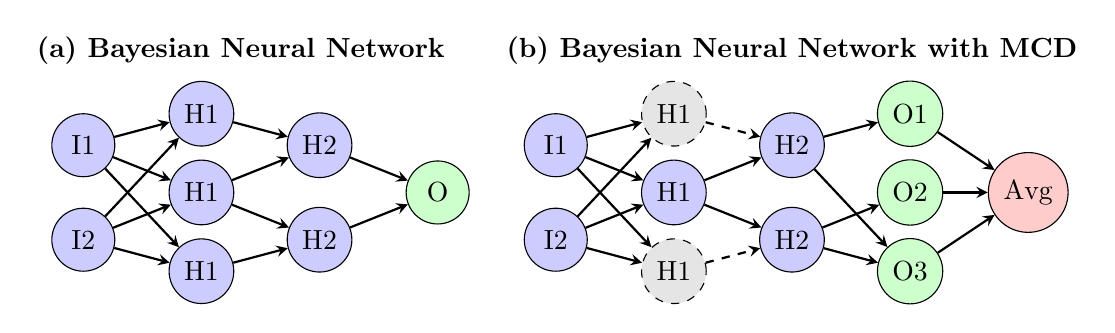
\begin{tikzpicture}[x=1.0cm, y=0.8cm, >=stealth]

        % === Standard Neural Network (Without MCD) ===
        \node[draw=none] at (2, 3) {\textbf{(a) Bayesian Neural Network}};

        % Input Layer (Left Side)
        \node[circle, draw, fill=blue!20, minimum size=0.8cm] (I1) at (0, 1.5) {I1};
        \node[circle, draw, fill=blue!20, minimum size=0.8cm] (I2) at (0, 0) {I2};

        % Hidden Layer 1 (No Dropout)
        \node[circle, draw, fill=blue!20, minimum size=0.8cm] (H11) at (1.5, 2) {H1};
        \node[circle, draw, fill=blue!20, minimum size=0.8cm] (H12) at (1.5, 0.75) {H1};
        \node[circle, draw, fill=blue!20, minimum size=0.8cm] (H13) at (1.5, -0.5) {H1};

        % Hidden Layer 2
        \node[circle, draw, fill=blue!20, minimum size=0.8cm] (H21) at (3, 1.5) {H2};
        \node[circle, draw, fill=blue!20, minimum size=0.8cm] (H22) at (3, 0) {H2};

        % Output Layer (Standard NN)
        \node[circle, draw, fill=green!20, minimum size=0.8cm] (O1) at (4.5, 0.75) {O};

        % Connections (Standard NN)
        \draw[->, thick] (I1) -- (H11);
        \draw[->, thick] (I1) -- (H12);
        \draw[->, thick] (I1) -- (H13);
        \draw[->, thick] (I2) -- (H11);
        \draw[->, thick] (I2) -- (H12);
        \draw[->, thick] (I2) -- (H13);

        \draw[->, thick] (H11) -- (H21);
        \draw[->, thick] (H12) -- (H21);
        \draw[->, thick] (H12) -- (H22);
        \draw[->, thick] (H13) -- (H22);

        \draw[->, thick] (H21) -- (O1);
        \draw[->, thick] (H22) -- (O1);

        \node[draw=none] at (9, 3) {\textbf{(b) Bayesian Neural Network with MCD}};

        \node[circle, draw, fill=blue!20, minimum size=0.8cm] (I1b) at (6, 1.5) {I1};
        \node[circle, draw, fill=blue!20, minimum size=0.8cm] (I2b) at (6, 0) {I2};
        
        \node[circle, draw, fill=gray!20, dashed, minimum size=0.8cm] (D1) at (7.5, 2) {H1};
        \node[circle, draw, fill=blue!20, minimum size=0.8cm] (D2) at (7.5, 0.75) {H1};
        \node[circle, draw, fill=gray!20, dashed, minimum size=0.8cm] (D3) at (7.5, -0.5) {H1};

        \node[circle, draw, fill=blue!20, minimum size=0.8cm] (H21b) at (9, 1.5) {H2};
        \node[circle, draw, fill=blue!20, minimum size=0.8cm] (H22b) at (9, 0) {H2};

        \node[circle, draw, fill=green!20, minimum size=0.8cm] (O1b) at (10.5, 2) {O1};
        \node[circle, draw, fill=green!20, minimum size=0.8cm] (O2b) at (10.5, 0.75) {O2};
        \node[circle, draw, fill=green!20, minimum size=0.8cm] (O3b) at (10.5, -0.5) {O3};

        \node[circle, draw, fill=red!20, minimum size=0.8cm] (Final) at (12, 0.75) {Avg};

        \draw[->, thick] (I1b) -- (D1);
        \draw[->, thick] (I1b) -- (D2);
        \draw[->, thick] (I1b) -- (D3);
        \draw[->, thick] (I2b) -- (D1);
        \draw[->, thick] (I2b) -- (D2);
        \draw[->, thick] (I2b) -- (D3);

        \draw[->, thick, dashed] (D1) -- (H21b);
        \draw[->, thick] (D2) -- (H21b);
        \draw[->, thick] (D2) -- (H22b);
        \draw[->, thick, dashed] (D3) -- (H22b);

        \draw[->, thick] (H21b) -- (O1b);
        \draw[->, thick] (H22b) -- (O2b);
        \draw[->, thick] (H21b) -- (O3b);
        \draw[->, thick] (H22b) -- (O3b);

        \draw[->, thick] (O1b) -- (Final);
        \draw[->, thick] (O2b) -- (Final);
        \draw[->, thick] (O3b) -- (Final);

    \end{tikzpicture}
    \caption{(a) Standard Neural Network: A traditional feed-forward structure with fixed weights. 
    (b) Neural Network with Monte Carlo Dropout (MCD): Dropout is applied during inference, producing different outputs across multiple forward passes, averaging to approximate Bayesian inference.}
    \label{fig:mcd_vs_standard}
\end{figure}

\noindent BNNs that employ Monte Carlo Dropout can efficiently produce both forecasts and uncertainty estimates. By using the expected forecast and uncertainty estimation, it is well usable in offshore weather forecasting. 

\section{Deep Learning Models, LSTM}
\label{lit:LSTM_literature}
Deep learning models can capture complex non-linear behaviour in time series forecasting. Given the large fluctuations in weather patterns over time and across regions, LSTMs offer a promising solution for improving forecast accuracy. A deep learning model, which is used in other forecasting applications, and on a smaller scale on weather, is long-short term memory, LSTM. The reason for usage is that it can capture both short-term fluctuations and long-term dependencies (\cite{siami2019comparison}). The model can be seen as a specific multi-layered type of artificial neural network, as explained in chapter \ref{lit:hybrid_models}. The differences lie in the recurrence inside this neural network, with feedback inside the system, it can retain information over time. The memory blocks inside the LSTM model are visualized in Figure \ref{fig:LSTM}.

\begin{figure}[h!]
    \centering
    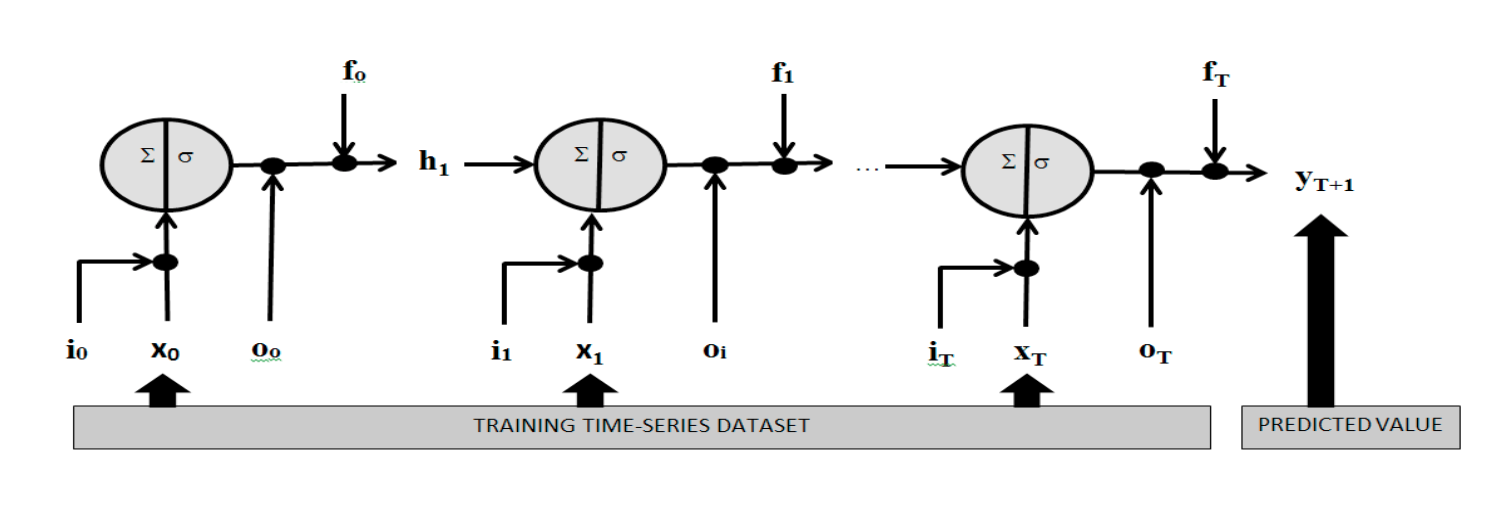
\includegraphics[width=1.0\linewidth]{images/LSTM.png}
    \caption{Architecture of Unfolded LSTM Model (\cite{salman2018single})}
    \label{fig:LSTM}
\end{figure}

\noindent As can be seen in Figure \ref{fig:LSTM} each LSTM block receives an input signal $x$, an input gate signal $i$, recurrent signal $h$, forget gate signal $f$ and produces an output gate signal $o$. LSTM networks compute a mapping of the input $(x_0,...,x_T)$ to an output sequence $(y_0,...,y_T)$ (\cite{salman2018single}). This is done by calculating the network unit activations using the following formulas (\cite{hochreiter1997long}). 

\begin{equation}
    i_t = \sigma(W_i x_t + U_i h_{t-1} + b_i)
    \label{eq:3}
\end{equation}

\begin{equation}
    z_t = \tanh(W_z x_t + U_z h_{t-1} + b_z)
    \label{eq:4}
\end{equation}

\begin{equation}
    f_t = \sigma(W_f x_t + U_f h_{t-1} + b_f)
    \label{eq:5}
\end{equation}

\begin{equation}
    C_t = i_t * z_t + f_t * C_{t-1}
    \label{eq:6}
\end{equation}

\begin{equation}
    o_t = \sigma(W_o x_t + U_o h_{t-1} + V_o C_t + b_o)
    \label{eq:7}
\end{equation}

\begin{equation}
    h_t = o_t * \tanh(C_t)
    \label{eq:8}
\end{equation}

\noindent Standard recurrent neural networks often suffer from the vanishing gradient problem, which is a disadvantage when learning over long sequences of data. LSTMs mitigate this issue by incorporating specialized gating mechanisms that preserve gradients over time (\cite{hochreiter1997long}). $W_i, U_i, W_z, U_z, W_f, U_f, W_o$ and $U_o$ are all model parameters which need to be estimated during training of the model with known data. While this model has some increase in computational time, the benefit of a more accurate model is in this case prioritized (\cite{salman2018single}). 

\vspace{0.25cm}

\noindent The memory cell, $C_t$, in combination with the input, forget, and output gates enables the LSTM to hold valuable information over long durations while discarding less relevant data. This design is key to its ability to capture long-term dependencies and adapt to rapid changes in weather conditions, making it suitable for forecasting in dynamic offshore environments.

\section{Comparative Analysis}
\label{lit:comparative}
Although historical models like NWP, SF and EF provide a good foundation for weather forecasting and give relatively accurate results, it is important to look at their shortcomings. For the usage in offshore wind turbine installation, it is important that the models can be easily adapted to fluctuating data. This is where these models are less efficient in terms of handling non-linear patterns, accuracy for long-term forecasts and localized forecasts. Offshore weather forecasting needs models which can predict dynamic and local conditions but also need to be able to adapt quickly to sudden changes (\cite{Zhang2019}).

\vspace{0.25cm}

\noindent From this follows the reason to investigate new applicable models. In the research, the focus will be on 3 different types of models. Firstly, a hybrid model consisting of the historical model ARIMA, for linear behaviour, and combining this with a new ANN, to capture non-linear behaviour. This model is highly suitable in environments where both smooth trends and abrupt changes occur. Research has shown that hybrid models can significantly improve forecast accuracy by combining the strengths of statistical and machine learning approaches (\cite{zhang2003time}, \cite{buyuksahin2019improving}). Secondly, a probabilistic model in the form of BNN. By incorporating Monte Carlo Dropout, the BNN efficiently approximates Bayesian inference, offering a predictive distribution that quantifies uncertainty-making in highly variable offshore conditions (\cite{gal2016dropout}, \cite{mae2022uncertainty}). Finally, a deep-learning model in the form of an LSTM. LSTM networks have proven effective in various forecasting applications due to their ability to model both short-term fluctuations and long-term dependencies in time series data (\cite{siami2019comparison}). All strengths and Limitations are shown in Table \ref{table:comparative_models}. 

\begin{table}[h!]
\centering
\caption{Comparative Analysis of Advanced Forecasting Models for Offshore Applications}
\label{table:comparative_models}
\begin{tabular}{|p{2cm}|p{6.3cm}|p{6cm}|}
\hline
\centering \textbf{Model} & \textbf{Strengths} & \textbf{Weaknesses} \\ \hline 
\vspace{5pt}
\centering\textbf{ARIMA-ANN} & 
Based on ARIMA's ability to capture linear trends\newline
Augmented by ANN's capacity for non-linear pattern recognition\newline
Effective when both linear and non-linear fluctuations are present
& 
Requires careful tuning to balance ARIMA and ANN components\newline
Performance depends on the quality of ARIMA residuals \\ \hline
\vspace{5pt}
\centering\textbf{BNN (with MCD)} &
Provides probabilistic forecasts with uncertainty quantification\newline
Facilitates risk assessment in dynamic offshore conditions
& 
Complex implementation and interpretation\newline
Higher computational overhead than deterministic models \\ \hline
\vspace{5pt}
\centering\textbf{LSTM} &
Excels at capturing long-term dependencies and complex dynamics\newline
Adept at modelling evolving non-linear time series data
& 
Requires large datasets and significant computational resources\newline
Maybe less interpretable compared to hybrid or probabilistic models \\ \hline
\end{tabular}
\end{table}

\noindent Since these comprehensive models demand more computation, their better accuracy and flexibility provide large benefits in forecasting the changing and localized conditions of offshore weather forecasting.

\section{Previous Research}
\label{lit:previous}
Earlier research has been done on the same subject by H. Boer and C. Overvliet, relevant findings, for this research, are included in this section.

\subsection{Research Boer}
The first research was done by H. Boer, the focus of this research was how the cost and installation time of offshore wind turbines are influenced by weather conditions. This was done with a numerical weather prediction, NWP, to simulate expected weather predictions and compare these with calm water situations. Key findings of this report are found in the influential met-ocean data on the installation face, these were significant wave height, wave frequency and wind speed. These parameters can have a maximum value, visible in Table \ref{table:operational_limits}, to ensure the installed ships can be used. 

\begin{table}[h!]
\centering
\caption{Operational Limits for Key Weather Conditions During Installation Phases}
\begin{tabular}{|l|c|c|c|c|c|c|}
\hline
\textbf{Phase} & \textbf{Vessel} & \textbf{Wave Height} & \textbf{Wave Frequency} & \textbf{Wind Speed} \\
\hline
\multirow{3}{*}{Monopile} & Crane Barge & 1.0 & 9 & 10 \\
 & HLV & 1.5 & 9 & 16 \\
 & Jack-Up & 2.5 & - & 16 \\
\hline
\multirow{3}{*}{Transition Piece} & Crane Barge & 1.0 & 9 & 10 \\
 & HLV & 1.5 & 9 & 16 \\
 & Jack-Up & 2.5 & - & 16 \\
\hline
\multirow{3}{*}{Tower} & Crane Barge & 1.0 & 7 & 10 \\
 & HLV & 1.5 & 7 & 10 \\
 & Jack-Up & 2.5 & - & 10 \\
\hline
\multirow{3}{*}{Nacelle} & Crane Barge & 1.0 & 7 & 10 \\
 & HLV & 1.5 & 7 & 10 \\
 & Jack-Up & 2.5 & - & 10 \\
\hline
\multirow{3}{*}{Blade} & Crane Barge & 1.0 & 7 & 8 \\
 & HLV & 1.5 & 7 & 8 \\
 & Jack-Up & 2.5 & - & 8 \\
\hline
\end{tabular}
\label{table:operational_limits}
\end{table}

\noindent Overall the report emphasizes how important accurate weather forecasting is in the installation phase of offshore wind turbines to minimize delays and so reduce costs. The simulated model underscores the importance of accurate weather forecasting, where this research compares calm weather with weather-restricted scenarios, it becomes clear why accurate weather forecasting is necessary (\cite{boer2022installation}).

\subsection{Research Overvliet}
The second research was conducted by C. Overvliet, this study focuses on quantifying the impact of increasing uncertainty in the weather forecasts on the delays and costs associated with the installation phase of offshore wind turbines. In this research, one specific location in the North Sea was used for data training, learning and testing. The models used are an Artificial Neural Network (ANN), an Auto-Regressive Integrated Moving Average (ARIMA), and a Long-Short Term Memory (LSTM). All these models are evaluated separately to determine their effectiveness in predicting weather conditions. 
\\

\noindent Where ARIMA models only showed the linear trends, it was chosen to further investigate the non-linear behaviours in the data. With high variability in the weather, such as sudden changes in wind speed and wave height, it showed the ANN and LSTM models made more accurate forecasts. ANN provided a model which identifies the non-linear relationship between the different influential variables. While LSTM offered an extra advantage in capturing long-term dependencies in the met-ocean data. 
\\

\noindent Another key finding in the report shows the relationship between the forecast accuracy and how this directly impacts the scheduling and associated costs of the installation phase. The greater the uncertainty, the higher the operational costs that follow from delays due to weather constraints. Overall it shows the importance of reducing the accuracy and so having a smoother and more efficient operation (\cite{overvliet2023uncertainty}).
\chapter{Methodology}
In this Chapter, how the models are constructed will be elaborated, starting with the Data Collection in Section \ref{data_collection}. The data of site 15 will be split into two parts, 2001-2008 for the training, and 2009 and 2010 will be the testing years. The second Section \ref{mathematical models} shows the Mathematical equations for the three models. Together with the Flowcharts in Section\ref{flowcharts} they form the foundation on how the models are constructed. The actual Model Development will be elaborated on in Section \ref{model development}, first the data preprocessing, then the Hybrid ARIMA-ANN model, then the BNN with MCD model and finally the LSTM model. Finally, Section \ref{evaluation metrics method} explains how the models can be quantified and which Evaluation Metrics are used for this. 

\section{Data Collection}
\label{data_collection}
The data will be used for the model's training/learning and testing phases. One site, 15 North Sea Center, is used for measurements, with the help of buoys equipped with sensors. The site gathered information for 10 years, with a measurement of each hour of each day for a total of 87,600 data points. An example of one time step of the measurements can be seen in Table \ref{table:metocean_data}. The depth of the site is $29$ meters and is located in the middle of the North Sea, Figure \ref{fig:location buoys} shows the location of site 15. For seabed wind turbines, which are installed between $0-30$ meters, it would not be relevant to investigate deeper sites (\cite{DNV2018}).

\begin{figure}[ht!]
    \centering
    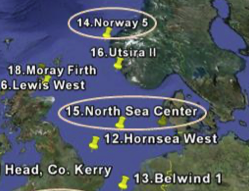
\includegraphics[width=0.4\linewidth]{images/Location buoys.png}
    \caption{Location buoys (\cite{lin2015joint})}
    \label{fig:location buoys}
\end{figure}

\begin{table}[ht!]
\centering
\caption{Met-ocean Data hour 1}
\renewcommand{\arraystretch}{1.5} % Adjust row spacing
\resizebox{\textwidth}{!}{%
\begin{tabular}{|c|c|c|c|c|c|c|c|c|}
\hline
\textbf{nx} & \textbf{ny} & \textbf{datetime} & \textbf{s\_wht} & \textbf{meanwdir} & \textbf{peak\_fr} & \textbf{mean\_fr} & \textbf{ustar} & \textbf{wind\_dir} \\
\hline
470 & 584 & 1/1/01 0:00 & 2.16 & 168.336 & 0.175 & 0.194 & 0.693 & 168.313 \\
\hline
\textbf{cdg} & \textbf{wind\_speed} & \textbf{depth} & \textbf{maxwh} & \textbf{maxwp} & \textbf{swe\_h} & \textbf{meansdir} & \textbf{meansfr} & \textbf{wsea\_h} \\
\hline
0 & 17.278 & 29 & 4.679 & 4.878 & 0.31 & 131.235 & 0.17 & 2.14 \\
\hline
\textbf{wsead} & \textbf{wsea\_fr} & \textbf{msp1} & \textbf{msp2} & \textbf{mwseap1} & \textbf{mwseap2} & & & \\
\hline
168.642 & 0.195 & 5.674 & 5.552 & 4.73 & 4.401 & & & \\
\hline
\end{tabular}%
}
\label{table:metocean_data}
\end{table}

\noindent From this data the significant wave height, $s_{wht}$, the wind speed, $wind_{speed}$, the mean frequency, $mean_{fr}$, and the datetime will be used. The reasoning follows from earlier research, Boer and Overvliet (\cite{boer2022installation}, \cite{overvliet2023uncertainty}), who already found the significance of these parameters in the installation phase of the turbines. While other parameters influence these key parameters, they fall beyond this project's scope. The installing ships can only be used when the values do not go over the operational limits of Table \ref{table:operational_limits}. The location of the site can be seen in Figure \ref{fig:location buoys}, site $15$ corresponds to a depth of $29$ meters. \\

\noindent To show the relevance of these models in respect to the jack-up vessels maximum values-on the significant wave heigth $=2.5$ [meters], the wind speed $=16$, $10$ and $8$ [meters per second] and the mean period for the crane barge or the heavy lift vehicle (HVL) $=9$ and $7$ [seconds]-these values over the mean of the available data is shown in Figure \ref{fig:site15_limits}. Some trends are already visible in these figures. Firstly, seasonality where hour $0$ represents the $1^{st}$ of January at 00:00. The peaks at the winter months are significantly higher than those in summer. Another recurring trend is the increasing difference between the minimum and maximum values of each peak over time. This is especially visible in the significant wave height and the mean frequency, which can probably be linked to the tides. 

\begin{figure}[h!]
    \centering
    \begin{subfigure}[b]{0.47\textwidth}
        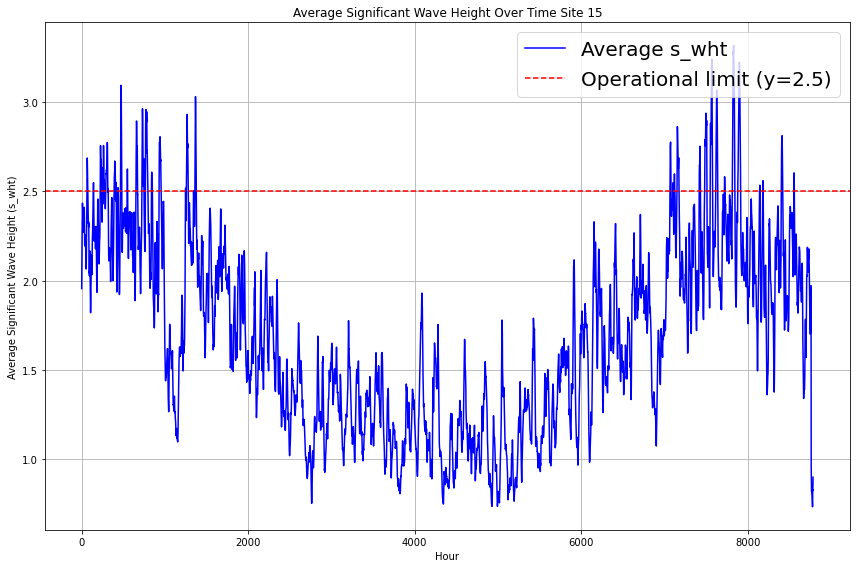
\includegraphics[width=\textwidth]{graphs/s_wht_limit_site_15.png} 
        \caption{Significant Wave Height}
        \label{fig:s_wht_15}
    \end{subfigure}
    \hfill
    \begin{subfigure}[b]{0.47\textwidth}
        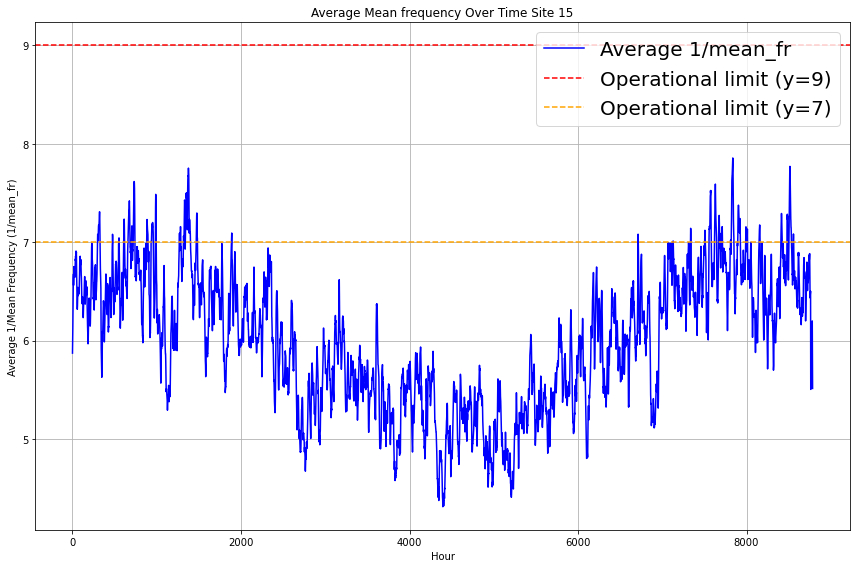
\includegraphics[width=\textwidth]{graphs/mean_fr_limit_site_15.png} 
        \caption{Mean Frequency}
        \label{fig:mean_fr_15}
    \end{subfigure}
    \vskip\baselineskip
    \begin{subfigure}[b]{0.47\textwidth}
        \centering
        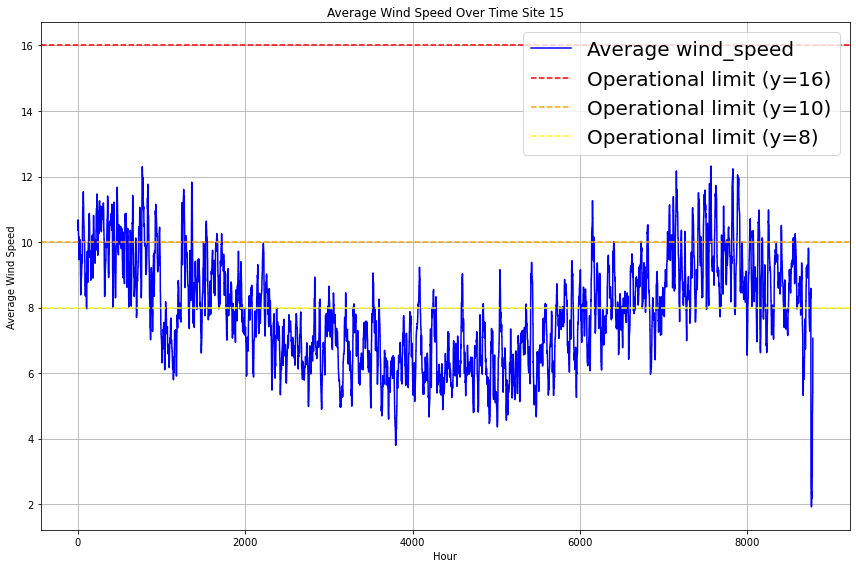
\includegraphics[width=\textwidth]{graphs/wind_speed_limit_site_15.png} 
        \caption{Wind Speed}
        \label{fig:wind_speed_15}
    \end{subfigure}
    \caption{Site 15 key parameters over time compared with operational limits}
    \label{fig:site15_limits}
\end{figure}

\newpage

\section{Mathematical Models}
\label{mathematical models}
This section will show the mathematical models specified for the inputted data and made for each model separately. To forecast the significant wave height ($s_{wht}$), the mean wave frequency ($mean_{fr}$), and the wind speed ($wind_{speed}$). 

\subsection{Mathematical model: Hybrid ARIMA–ANN Model}
\label{math:hybrid}
\noindent \textbf{ARIMA Component:}  
For each target variable, the ARIMA model is defined as:
\begin{equation}
    y(t) = \phi(B) \, y(t) + \theta(B) \, a_t,
    \label{eq:arima_generic}
\end{equation}
Where:
\begin{itemize}
    \item \(\phi(B)\) is the autoregressive polynomial,
    \item \(\theta(B)\) is the moving average polynomial,
    \item \(a_t\) denotes white noise,
    \item \(B\) is the backshift operator.
\end{itemize}

\noindent The residual error from the ARIMA model is computed as:
\begin{equation}
    e(t) = y(t) - \hat{y}_{ARIMA}(t),
    \label{eq:residual_error2}
\end{equation}
where \(\hat{y}_{ARIMA}(t)\) is the forecast produced by the ARIMA model.\\

\noindent \textbf{ANN Component:}  
The Artificial Neural Network (ANN) is used to model the nonlinear component of the time series. For a neuron \(j\) in layer \(l\), the activation is defined as:
\begin{equation}
    z^{(l)}_j = \sigma\left(\sum_{i=1}^{n_{l-1}} w_{ij}^{(l)} z_i^{(l-1)} + b_j^{(l)}\right),
    \label{eq:activation_function}
\end{equation}
Where:
\begin{itemize}
    \item \(w_{ij}^{(l)}\) and \(b_j^{(l)}\) are the weights and biases of layer \(l\),
    \item \(\sigma(\cdot)\) denotes an activation function (e.g., sigmoid or ReLU).
\end{itemize}

The output of the ANN is given by:
\begin{equation}
    y_{\text{ANN}}(t) = f(X),
    \label{eq:ann_output}
\end{equation}
with \(X\) representing a sliding window of past values from the same time series.\\

\noindent \textbf{Hybrid Forecast:}  
The final hybrid forecast is obtained by combining the ARIMA and ANN forecasts:
\begin{equation}
    y_{\text{hybrid}}(t) = \hat{y}_{ARIMA}(t) + y_{\text{ANN}}(t).
    \label{eq:hybrid_forecast2}
\end{equation}

\subsection{Mathematical model: Bayesian Neural Network with MC Dropout}
\label{math:BNN}

Let \( f(X, w) \) denote the output of a neural network for input \( X \) and weights \( w \). In our Bayesian Neural Network (BNN) framework, the weights are treated as random variables with an approximate posterior distribution \( q(w) \). Instead of performing full Bayesian inference, we use Monte Carlo Dropout to approximate this distribution during inference.\\

\noindent During a single forward pass with dropout active, the network function is computed as follows:
\begin{align}
    z^{(1)} &= \text{ReLU}(W^{(1)} X + b^{(1)}) \odot \xi, \label{eq:dropout_layer1}\\[1mm]
    z^{(2)} &= \text{ReLU}(W^{(2)} z^{(1)} + b^{(2)}), \label{eq:dropout_layer2}\\[1mm]
    \hat{y} &= W^{(3)} z^{(2)} + b^{(3)}, \label{eq:network_output}
\end{align}
Where:
\begin{itemize}
    \item \(W^{(l)}\) and \(b^{(l)}\) are the weight matrix and bias vector for layer \(l\),
    \item \(\text{ReLU}(\cdot)\) is the Rectified Linear Unit activation function,
    \item \(\xi\) is a dropout mask applied element-wise, with each element sampled from a Bernoulli distribution \(\text{Bernoulli}(1-p)\), where \(p\) is the dropout rate,
    \item The operator \(\odot\) denotes element-wise multiplication.
\end{itemize}

\noindent To approximate the predictive distribution, we perform \(N\) stochastic forward passes, each with independent dropout masks. The final prediction is obtained by averaging these Monte Carlo samples:
\begin{equation}
    \hat{y}_{\text{MC}} = \frac{1}{N} \sum_{i=1}^{N} f(X, w_i),
    \label{eq:mc_dropout_prediction}
\end{equation}
where each \(w_i\) represents a set of weights resulting from a different dropout mask.

\noindent This procedure approximates Bayesian inference by effectively sampling from the approximate posterior \(q(w)\) and provides both a mean prediction and a measure of uncertainty.

\subsection{Mathematical model: LSTM}
\label{math:LSTM}
The Long Short-Term Memory (LSTM) network is designed to capture both short-term fluctuations and long-term dependencies in time series data. An LSTM unit is defined by the following set of equations:
\begin{align}
    i_t &= \sigma\left(W_i x_t + U_i h_{t-1} + b_i\right), \label{eq:lstm_input}\\[1mm]
    f_t &= \sigma\left(W_f x_t + U_f h_{t-1} + b_f\right), \label{eq:lstm_forget}\\[1mm]
    o_t &= \sigma\left(W_o x_t + U_o h_{t-1} + b_o\right), \label{eq:lstm_output}\\[1mm]
    \tilde{C}_t &= \tanh\left(W_C x_t + U_C h_{t-1} + b_C\right), \label{eq:lstm_candidate}\\[1mm]
    C_t &= f_t \odot C_{t-1} + i_t \odot \tilde{C}_t, \label{eq:lstm_cell}\\[1mm]
    h_t &= o_t \odot \tanh\left(C_t\right), \label{eq:lstm_hidden}
\end{align}
where:
\begin{itemize}
    \item \(x_t\) is the input at time \(t\),
    \item \(h_t\) is the hidden state at time \(t\),
    \item \(C_t\) is the cell state at time \(t\),
    \item \(i_t\), \(f_t\), and \(o_t\) denote the input, forget, and output gates respectively,
    \item \(W_i, W_f, W_o, W_C\) are the weight matrices for the input,
    \item \(U_i, U_f, U_o, U_C\) are the recurrent weight matrices,
    \item \(b_i, b_f, b_o, b_C\) are the bias vectors,
    \item \(\sigma(\cdot)\) is the sigmoid activation function,
    \item \(\tanh(\cdot)\) denotes the hyperbolic tangent function,
    \item \(\odot\) represents element-wise multiplication.
\end{itemize}

For forecasting, a sequence-to-one architecture is employed:
\[
\hat{y}(t) = f_{\text{LSTM}}(x_{t-k}, \ldots, x_{t-1}),
\]
where \(\{x_{t-k}, \ldots, x_{t-1}\}\) is the input sequence of length \(k\) and \(\hat{y}(t)\) is the forecast at time \(t\).

\section{Flowchart}
\label{flowcharts}
To clarify the construction and operational framework of the forecasting models, flowcharts for each approach are presented. These diagrams serve as visual guides that outline the step-by-step development process, ensuring that each model is built systematically and functions as intended.

\begin{center}
\begin{tikzpicture}[node distance=0.5cm, auto,
    block/.style={draw, rectangle, rounded corners, fill=blue!20, align=center, minimum width=3cm, minimum height=1cm},
    arrow/.style={->, thick, >=stealth}]

    \node[block] (preprocess) {Data Preprocessing};
    \node[font=\bfseries, above=0.3cm of preprocess, align=center] (title) {Hybrid ARIMA–ANN Model Framework};
    \node[block, below left=of preprocess, xshift=-1.4cm] (arima) {ARIMA Model\\(Linear Forecast)};
    \node[block, below right=of preprocess, xshift=1.4cm] (ann) {ANN Model\\(Nonlinear Forecast)};
    \node[block, below=of preprocess, yshift=-1cm] (hybrid) {Hybrid Forecast\\\(\hat{y}_{ARIMA} + y_{ANN}\)};
    \node[block, below=of hybrid] (refit) {Model Refit \& Error Calculation};
    \node[block, below=of refit] (rolling) {Rolling Update\\ \& Forecasting Loop};
    \node[block, below=of rolling] (evaluation) {Evaluation};

    \draw[arrow] (preprocess) -- (arima);
    \draw[arrow] (preprocess) -- (ann);
    \draw[arrow] (arima) to node[above]{\shortstack{Residual error:\\ \(e(t)=y(t)-\hat{y}_{ARIMA}(t)\)}} (ann);
    \draw[arrow] (arima) -- (hybrid);
    \draw[arrow] (ann) -- (hybrid);
    \draw[arrow] (hybrid) -- (refit);
    \draw[arrow] (refit) -- (rolling);
    \draw[arrow] (rolling) -- (evaluation);
    
\end{tikzpicture}
\end{center}

\begin{center}
\begin{tikzpicture}[node distance=0.5cm, auto,
    block/.style={draw, rectangle, rounded corners, fill=blue!20, align=center, minimum width=3cm, minimum height=1cm},
    arrow/.style={->, thick, >=stealth}]

    \node[block] (preprocess_bnn) {Data Preprocessing};
    \node[block, below=of preprocess_bnn] (bnn) {BNN with MC Dropout\\(Stochastic Forward Passes)};
    \node[block, below=of bnn] (aggregation) {Aggregation of MC Samples\\(Final Forecast)};
    \node[block, below=of aggregation] (refit_bnn) {Model Refit \& Error Calculation};
    \node[block, below=of refit_bnn] (rolling_bnn) {Rolling Update \& Forecast Loop};
    \node[block, below=of rolling_bnn] (evaluation_bnn) {Evaluation};

    \node[above=0.3cm of preprocess_bnn, font=\bfseries] {BNN with MC Dropout Model};
    
    \begin{scope}[xshift=8cm]
        \node[block] (preprocess_lstm) {Data Preprocessing};
        \node[block, below=of preprocess_lstm] (lstm_train) {LSTM Training\\(Sequence-to-One)};
        \node[block, below=of lstm_train] (forecast_lstm) {LSTM Forecasting};
        \node[block, below=of forecast_lstm] (refit_lstm) {Model Refit \& Error Calculation};
        \node[block, below=of refit_lstm] (rolling_lstm) {Rolling Update \& Forecast Loop};
        \node[block, below=of rolling_lstm] (evaluation_lstm) {Evaluation};

        \node[above=0.3cm of preprocess_lstm, font=\bfseries] {LSTM Model};
    \end{scope}

    \draw[arrow] (preprocess_bnn) -- (bnn);
    \draw[arrow] (bnn) -- (aggregation);
    \draw[arrow] (aggregation) -- (refit_bnn);
    \draw[arrow] (refit_bnn) -- (rolling_bnn);
    \draw[arrow] (rolling_bnn) -- (evaluation_bnn);
    
    \draw[arrow] (preprocess_lstm) -- (lstm_train);
    \draw[arrow] (lstm_train) -- (forecast_lstm);
    \draw[arrow] (forecast_lstm) -- (refit_lstm);
    \draw[arrow] (refit_lstm) -- (rolling_lstm);
    \draw[arrow] (rolling_lstm) -- (evaluation_lstm);
    
\end{tikzpicture}
\end{center}

\newpage

\section{Model Development}
\label{model development}
This section describes how each model was built and trained, including the preprocessing, the hyperparameter choosing and the rolling refit strategies. 

\subsection{Data Preprocessing}
Before training the forecasting models and constructing the different scripts, it is essential to preprocess the inputted data. This needs to be done to ensure the learning algorithms of the models receive consistent and meaningful data. Five different steps are taken before the data can be used. Beginning with the handling of missing values, by implementing linear interpolation, these values can be estimated. When a value is not available, past values are used to bridge the gaps in the inputted data. Secondly, leap days are removed from the data, while this would give different sizes of inputted data, which will be mishandled by the models.\\

\noindent Each parameter is then scaled to normalise the inputted data. This is done to make the gradient-based optimizers in the scripts converge faster. The normalization parameters are then saved and will be used for the testing of the refitted data. A second reason to perform this normalization is to ensure that each variable exerts a balanced influence on the model.
The data is split into two, the years 2001-2008 will be used as training years for the models. The data for 2009-2010 will be used as the testing years. This clear split is done to ensure there is no accidental data leakage in the construction of the forecasts.\\

\noindent Finally, a refit interval of five days is used to be able to make a rolling forecast without exceeding the computational time. After each five days, the new observations of the actual data are added to the rolling windows. These rolling windows are then used to update the whole model, so instead of using all available data to reconstruct a new model, the old model is updated with this new data. 

\subsection{Hybrid ARIMA-ANN Model Development}
To develop the Hybrid model, the flowchart from Chapter \ref{flowcharts} and the mathematical model from Chapter \ref{math:hybrid} are used. Two site-by-site models need to be created, one for the linear components of the data and one for the non-linear components. This is all done to eventually forecast the significant wave height, $s_{wht}$, the mean wave frequency, $mean_{fr}$, and the wind speed $wind_{speed}$.\\ 

\noindent First, the ARIMA model, from Formula \ref{eq:arima_generic}, to find a good configuration between the autoregressive, diverging and moving average part, an iterative process is performed. During the process, it is found that [2 0 3] would give a minimal mean squared error concerning the actual data. The ARIMA is then fitted over the historical data and will produce a \(\hat{y}_{ARIMA}(t)\). This is used to then calculate the residuals, Formula \ref{eq:residual_error2}, which will capture the parts ARIMA did not forecast.\\

\noindent This residual, \(e(t)\), will be the input for the non-linear, ANN, component of the model. The different number of hidden layers inside the ANN is found through an iterative process, that is why \(s_{wht}\) will have 5 hidden neurons, but \(mean_{fr}\) and \(wind_{speed}\) will have 15 hidden neurons. A training function is the Levenberg-Marquardt algorithm, which has a maximum number of epochs, the upper limit on the number of training iterations, and an error goal. The algorithm minimizes the mean squared error by iteratively adjusting the network weights and biases, this is done until the error goal is reached or the maximum number of epochs is used (\cite{hagan1994training}). Then it is used to predict \(y_{ANN}(t)\), when combined with  \(\hat{y}_{ARIMA}(t)\) the final hybrid forecast is obtained with Formula \ref{eq:hybrid_forecast2}.

\subsection{Bayesian Neural Network with MC Dropout Model Development}
The BNN with MC dropout network was constructed based on the mathematical model in Chapter \ref{math:BNN}. Instead of separating linear and non-linear, the BNN with MC dropout will incorporate the uncertainty directly on the predictions.\\

\noindent The model designed construct a feed-forward neural network consisting of multiple hidden layers. Dropout layers are inserted between these hidden layers and will stay active during training. With the usage of MC dropout, the network is forced to randomly deactivate some neurons during each forward pass. This stochastic behaviour approximates sampling from an underlying posterior distribution over the network weights. 
During training, the network has the goal to minimize the mean squared error combined with the dropout. The reason this dropout is necessary is to prevent over-fitting. The configuration of the model, so the hidden layer structure, the maximum epochs, the dropout rate and the MC iterations, are found iteratively. Keeping a good balance between the models' accuracy and the computational time. The window size for \(s_{wht}\) and \(mean_{fr}\), so how much data is included during each forecast step, follows from the tides, which repeat every 149 hours (\cite{pugh1987tides}).\\

\noindent During the forecasting phase the model will perform multiple forward passes for each input. For input \(X\) this will lead to a set of outputs \(\{f(X,w_1),(f(X,w_2),...,(f(X,w_i)\}\). The final forecast is found by averaging all of these outputs using the Formula \ref{eq:mc_dropout_prediction}. Next to these forecasts, this will also give the variability among the predictions, which can be seen as the forecast uncertainty.

\subsection{LSTM Model Development}
Long Short-Term Memory model is designed to capture the short-term fluctuations and long-term dependencies of the inputted data. The LSTM model was constructed based on the flowchart, Chapter \ref{flowcharts} and the mathematical model Chapter \ref{math:LSTM}. As part of the data preprocessing for this model, input sequences are created with a sequence length of 48 hours. This can be related to the short-term trends in the met-ocean data. The reason to choose this two-day time-span follows from the weather patterns that can persist for multiple hours or even days. A sequence length of 48 hours allows the model to recognize storm development patterns, improving the ability to forecast extreme conditions more accurately. While longer sequences could capture extended dependencies, they must be balanced against computational cost. A 2-day window provides a reasonable trade-off between computational efficiency and forecasting accuracy. To ensure the long-term memory of the model is trained effectively, a 12-week rolling window is used. Both short-term fluctuations and long-term dependencies can be found in this weather window. In summary, for the short-term dependencies of the model, a 48-hour sequence is used. To capture the long-term dependencies, a 12-week rolling window is used, so the forecasts will be based on the most recent 12 weeks of data. \\

\noindent The LSTM architecture is designed to process the time series data efficiently. The hidden layers consist of 35 LSTM units, which will be constructed in the same manner as in Figure \ref{fig:LSTM}. Using fewer units may result in underfitting, where the model fails to capture important patterns in the data. While more units could be included, they do not significantly increase the accuracy, but they will increase the computational time. A fully connected layer is added in the model, this will ensure the dependencies in the past data are used to make a well-constructed final forecast. Finally, a regression layer is added, which minimizes the mean squared error (MSE) during training, reducing the overall difference between actual and predicted values. These layers contribute to a more accurate forecast model during the training phase.

\section{Evaluation Metrics}
\label{evaluation metrics method}
Each model makes a rolling forecast for each parameter separately, to compare these models to each other, evaluation metrics are used. The models are trained over the first 8 years of the available data, so from 2001 till 2008, this training is done based on minimizing the Mean Squared Error (MSE) in Formula \ref{eq:MSE2}. Although this is also used during the training, the metric itself is still useful to examine the accuracy of the models.

\begin{equation}
\label{eq:MSE2}
\text{MSE} = \frac{1}{N} \sum_{i=1}^{N} \left(y_i - \hat{y}_i\right)^2
\end{equation}

\noindent The Mean Absolute Error (MAE), Formula \ref{eq:MAE}, is used to reflect on the average magnitude of the forecast error. By using this metric, all deviations in the outcome will be treated equally. 

\begin{equation}
\label{eq:MAE}
\text{MAE} = \frac{1}{N} \sum_{i=1}^{N} \left|y_i - \hat{y}_i\right|
\end{equation}

\noindent Next to the MSE metric a Root Mean Squared Error (RMSE), Formula \ref{eq:RMSE}, like MSE, it will give a greater weight to larger errors. The reason to still use this follows from the fact that RMSE will penalize large errors more severely and so make it easier visible (\cite{hyndman2018forecasting}). 

\begin{equation}
\label{eq:RMSE}
\text{RMSE} = \sqrt{\frac{1}{N} \sum_{i=1}^{N} \left(y_i - \hat{y}_i\right)^2}
\end{equation}

\noindent Finally, to evaluate how accurate the forecast is to a naive baseline, a coefficient of determination ($R^2$), Formula \ref{eq:r^2}, is calculated. For this metric a value close to $1$ indicates the model captures a large part of the variance in the data. Negative values imply the model would be performing then the naive baseline (\cite{montgomery2012introduction}).

\begin{equation}
\label{eq:r^2}
R^2 = 1 - \frac{\sum_{i=1}^{N} \left(y_i - \hat{y}_i\right)^2}{\sum_{i=1}^{N} \left(y_i - \bar{y}\right)^2}
\end{equation}

%\section{Model Validation}
%\subsection{Validation Techniques}
%Description of various validation methods (e.g., cross-validation, holdout validation, time-series split) used for assessing model performance.

%\subsection{Training and Test Datasets}
%Explanation of how training and test datasets are selected and prepared.

%\subsection{Performance Metrics for Validation}
%Discussion of specific metrics used for validation (e.g., RMSE, MAE, R²) and their relevance in evaluating forecast accuracy.

\chapter{Results and Analysis}
This chapter shows the results of the different analyses made. Firstly, in Section \ref{comparitive_analysis} a comparative analysis of the Hybrid ARIMA-ANN model, BNN with MCD model and the LSTM model is made. To ensure consistency, a 5-day refit interval is used in each model. Section \ref{hybrid_model_results} shows how the Hybrid ARIMA-ANN model is performing under different refit intervals. This is done using a plot focusing on the evaluation metrics and a box plot showing the residual distribution. Finally, an implementation in the offshore installation of wind turbines is evaluated in Section \ref{implementation_results}, with the help of confusion matrices, the actual outcomes are analysed. 


\section{Comparative analysis}
\label{comparitive_analysis}
To compare the three different models, the hybrid ARIMA-ANN, BNN with MC dropout and LSTM, to one another, a 5-day refit interval is used. This is done to ensure all models will have the same input and that the differences in outcomes follow the differences in forecasting techniques. This will show which method is most effective in capturing the variability in the parameters, Significant Wave Height ($s_{wht}$), Mean Wave Frequency, ($mean_{fr}$) and Wind Speed ($wind_{speed}$). First, the different evaluation metrics can be seen in Table \ref{tab:performance_comparison}. Where the MSE was minimized during the training of each model, they will be very small overall compared to the other values. The BNN with MC dropout has higher values for the MAE, which suggests that the model might underfit or have a higher variability, compared to the other models. Also, the negative $R^2$ values occur when a model performs worse than a naive baseline. 

\begin{table}[ht!]
    \centering   
    \begin{tabular}{|l|c|c|c|c|}
        \hline
        \textbf{Parameter} & \textbf{Metrics} & \textbf{Hybrid} & \textbf{BNN with MCD} & \textbf{LSTM} \\
        \hline
        \textbf{Significant Wave Height}
        & MSE  & 0.0119 & 0.0162 & 0.0111 \\
        ($s_{wht}$) & MAE  & 0.0796 & 0.0923 & 0.0776 \\
        & RMSE & 0.1090 & 0.1273 & 0.1055 \\
        & R$^2$ & -0.0878 & -0.4838 & -0.0188 \\
        \hline
        \textbf{Mean Wave Frequency}
        & MSE  & 0.0134 & 0.0311 & 0.0115 \\
        ($mean_{fr}$) & MAE  & 0.0893 & 0.1410 & 0.0836 \\
        & RMSE & 0.1156 & 0.1765 & 0.1072 \\
        & R$^2$ & -0.0300 & -1.4003 & 0.1148 \\
        \hline
        \textbf{Wind Speed}
        & MSE  & 0.0187 & 0.0345 & 0.0186 \\
        ($wind_{speed}$) & MAE  & 0.1066 & 0.1446 & 0.1063 \\
        & RMSE & 0.1366 & 0.1858 & 0.1362 \\
        & R$^2$ & 0.0432 & -0.7698 & 0.0488 \\
        \hline
    \end{tabular}
    \caption{Performance comparison of Hybrid, BNN with MCD, and LSTM models.}
    \label{tab:performance_comparison}
\end{table}

\newpage

\noindent The difference between the models over a small zoomed in time window can be seen in Figure \ref{fig:combined_10day}. In this figure, it is visible how the models are constructed and performing over this small time frame. This time frame shows one refit interval in which the forecasted data is brought back to the actual values. The LSTM model, light blue line, tends to grow exponentially due to the way it is trained on the earlier data, from 2001 till 2008. This causes the model to not capture the fluctuations between the refit intervals. If the refit interval is increased further, the error between the actual values and the LSTM model will be larger. The BNN with MC dropout, the orange line, does capture the variability between the refit intervals and so follows the actual values better, the same can be seen for the Hybrid model, the red line. The difference between these two models is that the Hybrid model has a larger amplification, a larger fluctuation towards the mean, compared to the BNN with MC dropout model. Where the BNN with MC dropout follows the mean closer, the Hybrid model is less influenced by the averaged observed training data. 

\begin{figure}[ht!]
    \centering
    \begin{subfigure}[b]{0.49\textwidth}
        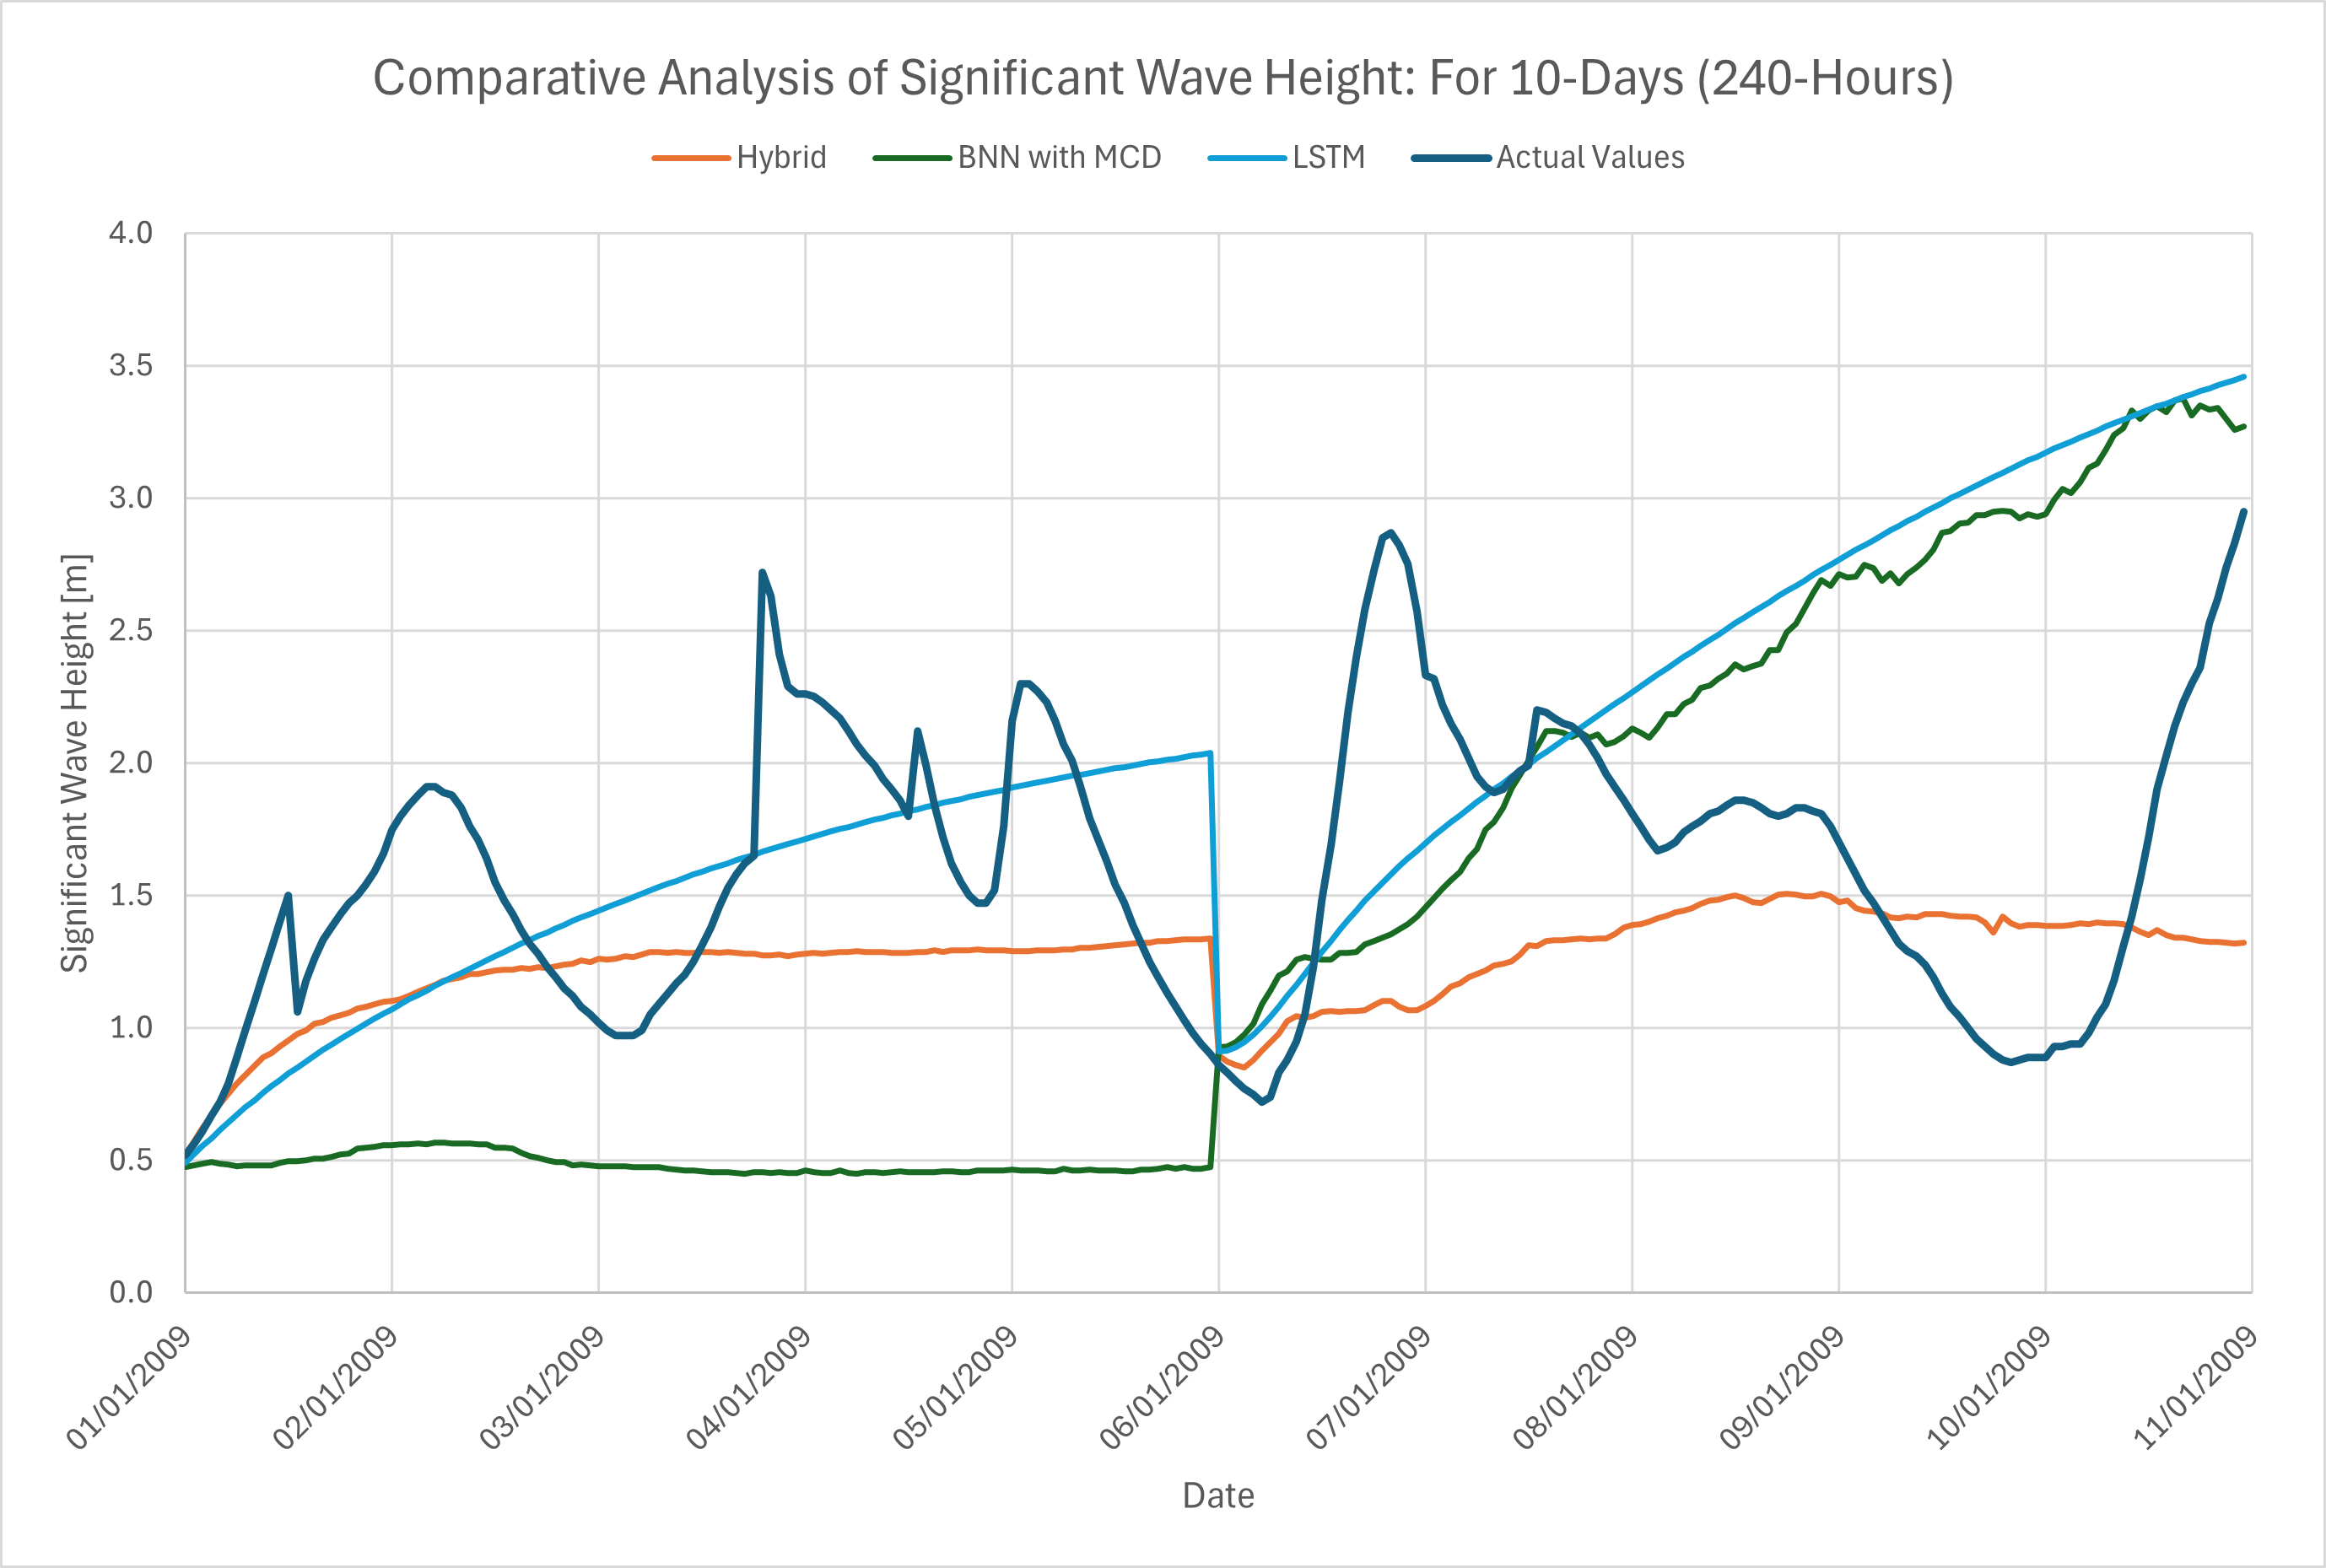
\includegraphics[width=\textwidth]{graphs/s_wht 240 hours.png}
        \caption{Significant Wave Height}
        \label{fig:s_wht_all_10Day}
    \end{subfigure}
    \hfill
    \begin{subfigure}[b]{0.49\textwidth}
        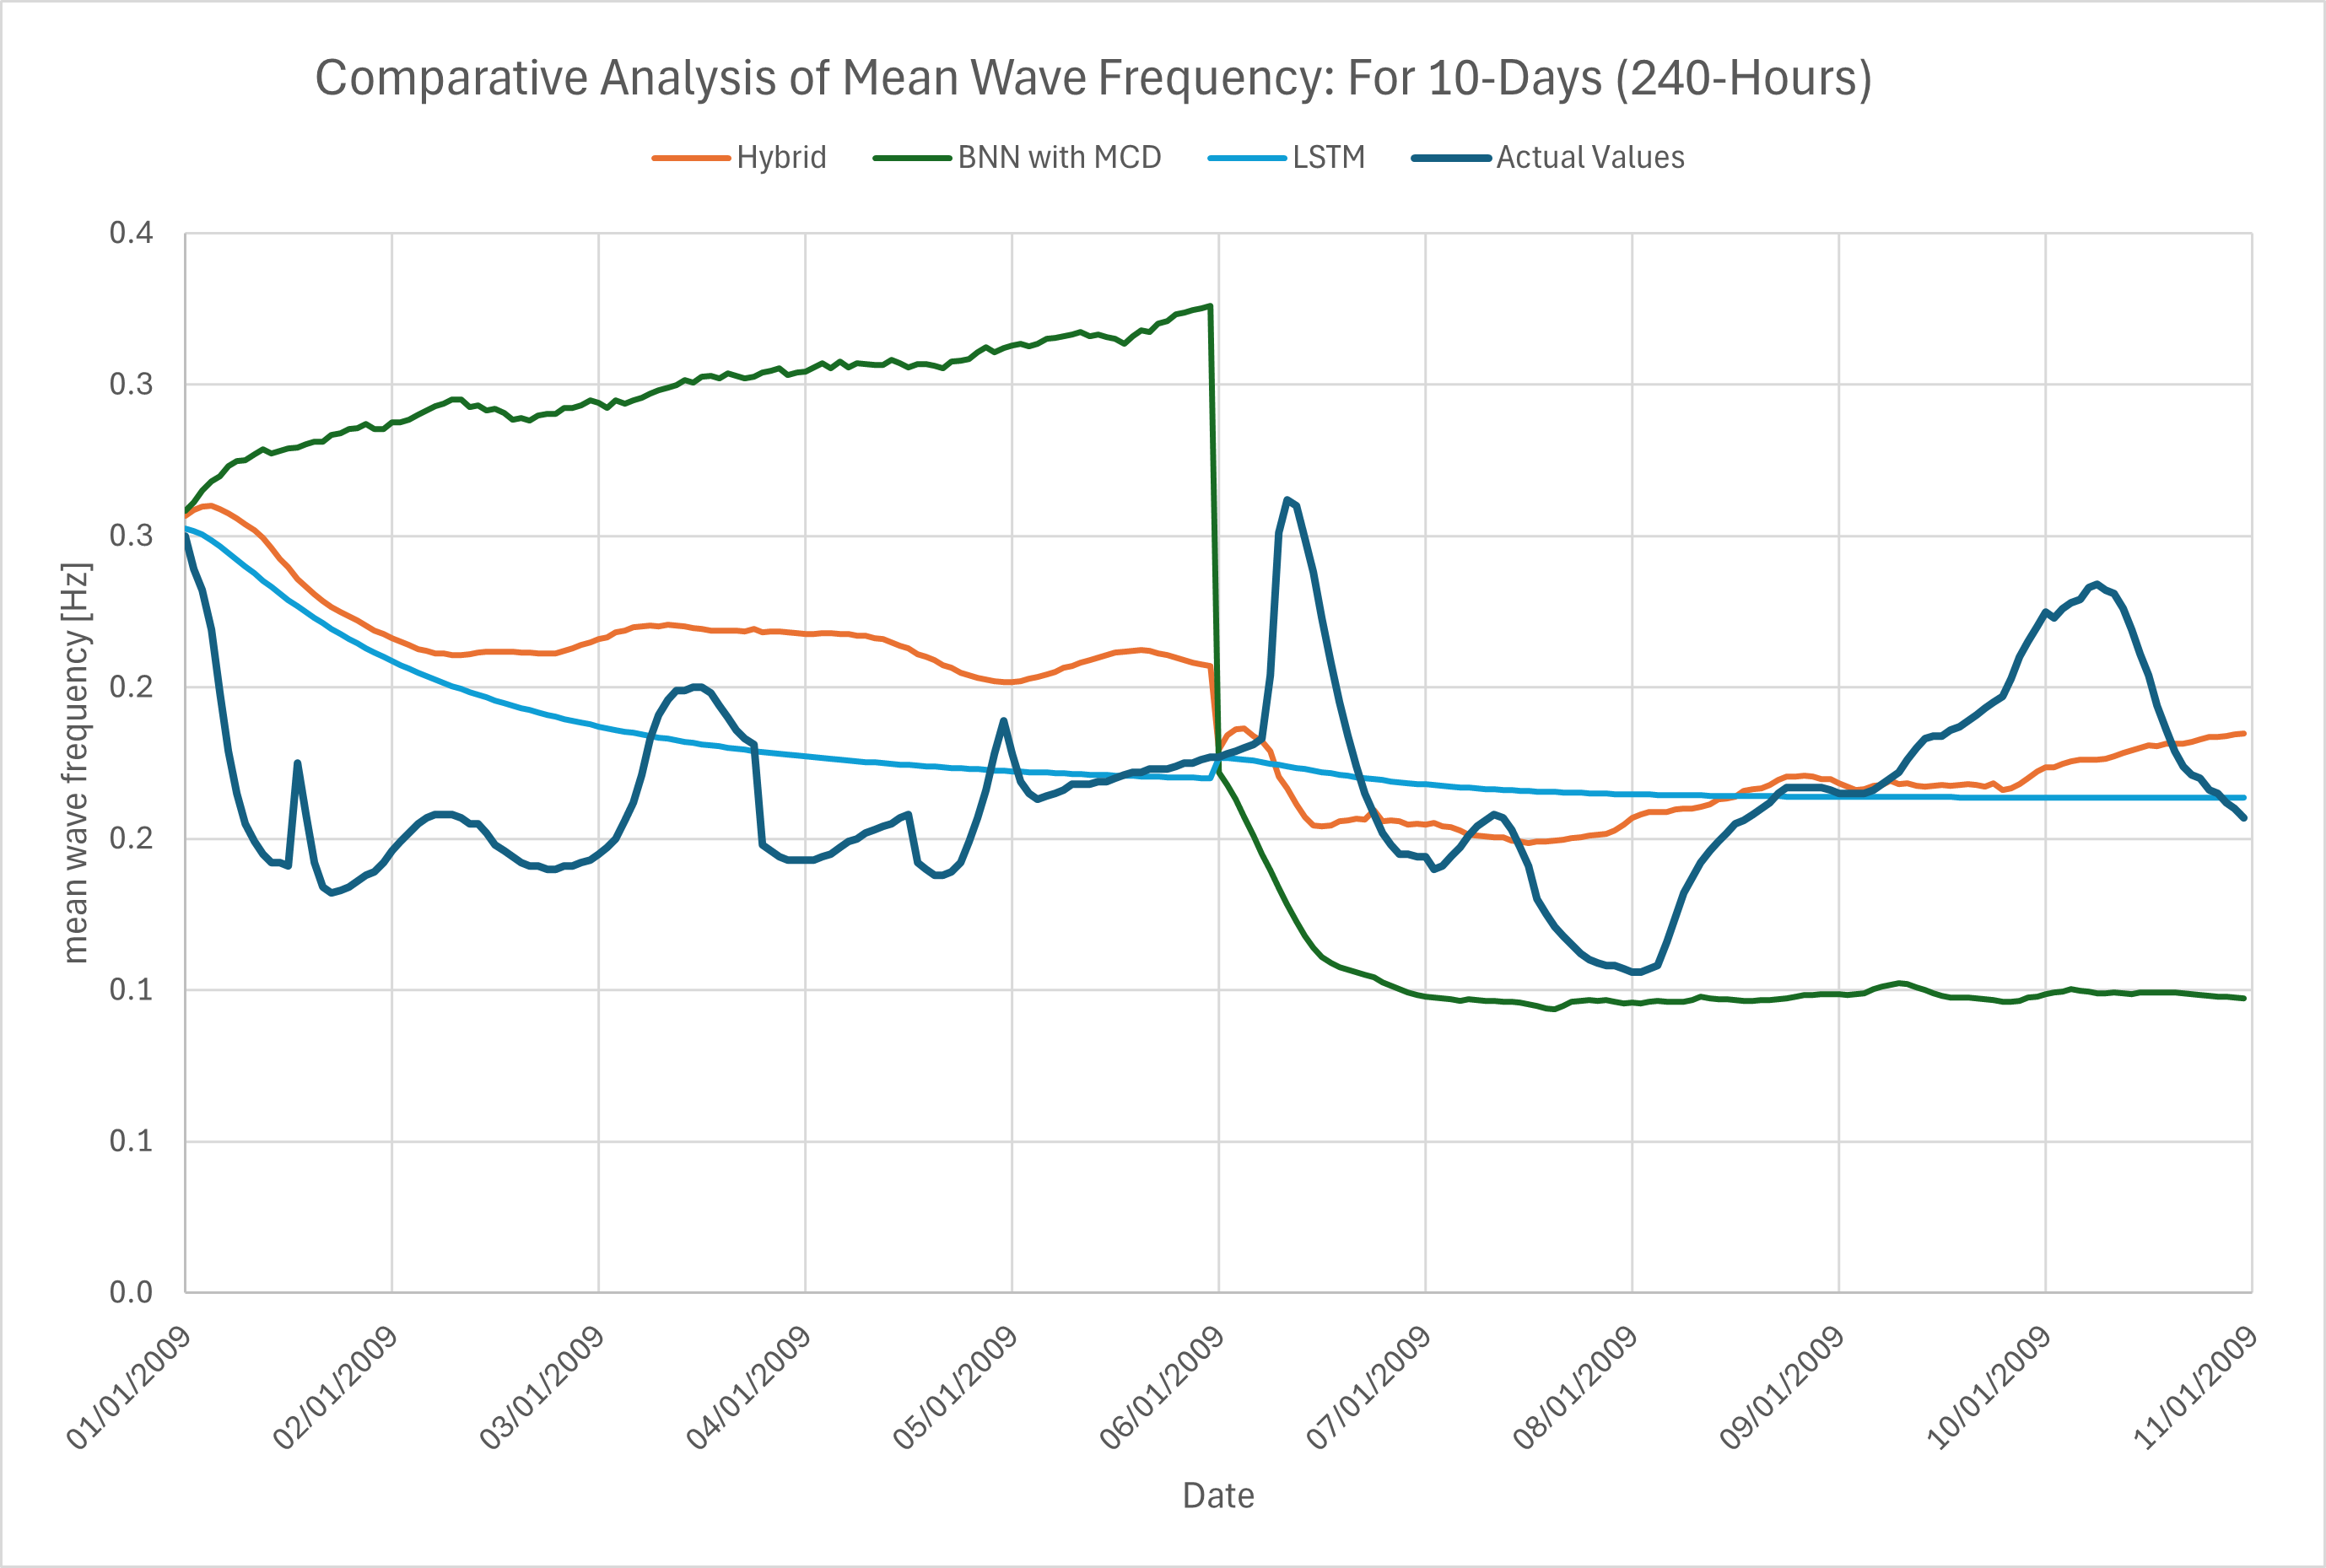
\includegraphics[width=\textwidth]{graphs/mean_fr 240 hours.png}
        \caption{Mean Wave Frequency}
        \label{fig:mean_fr_all_10Day}
    \end{subfigure}
    \vskip\baselineskip
    \begin{subfigure}[b]{0.49\textwidth}
        \centering
        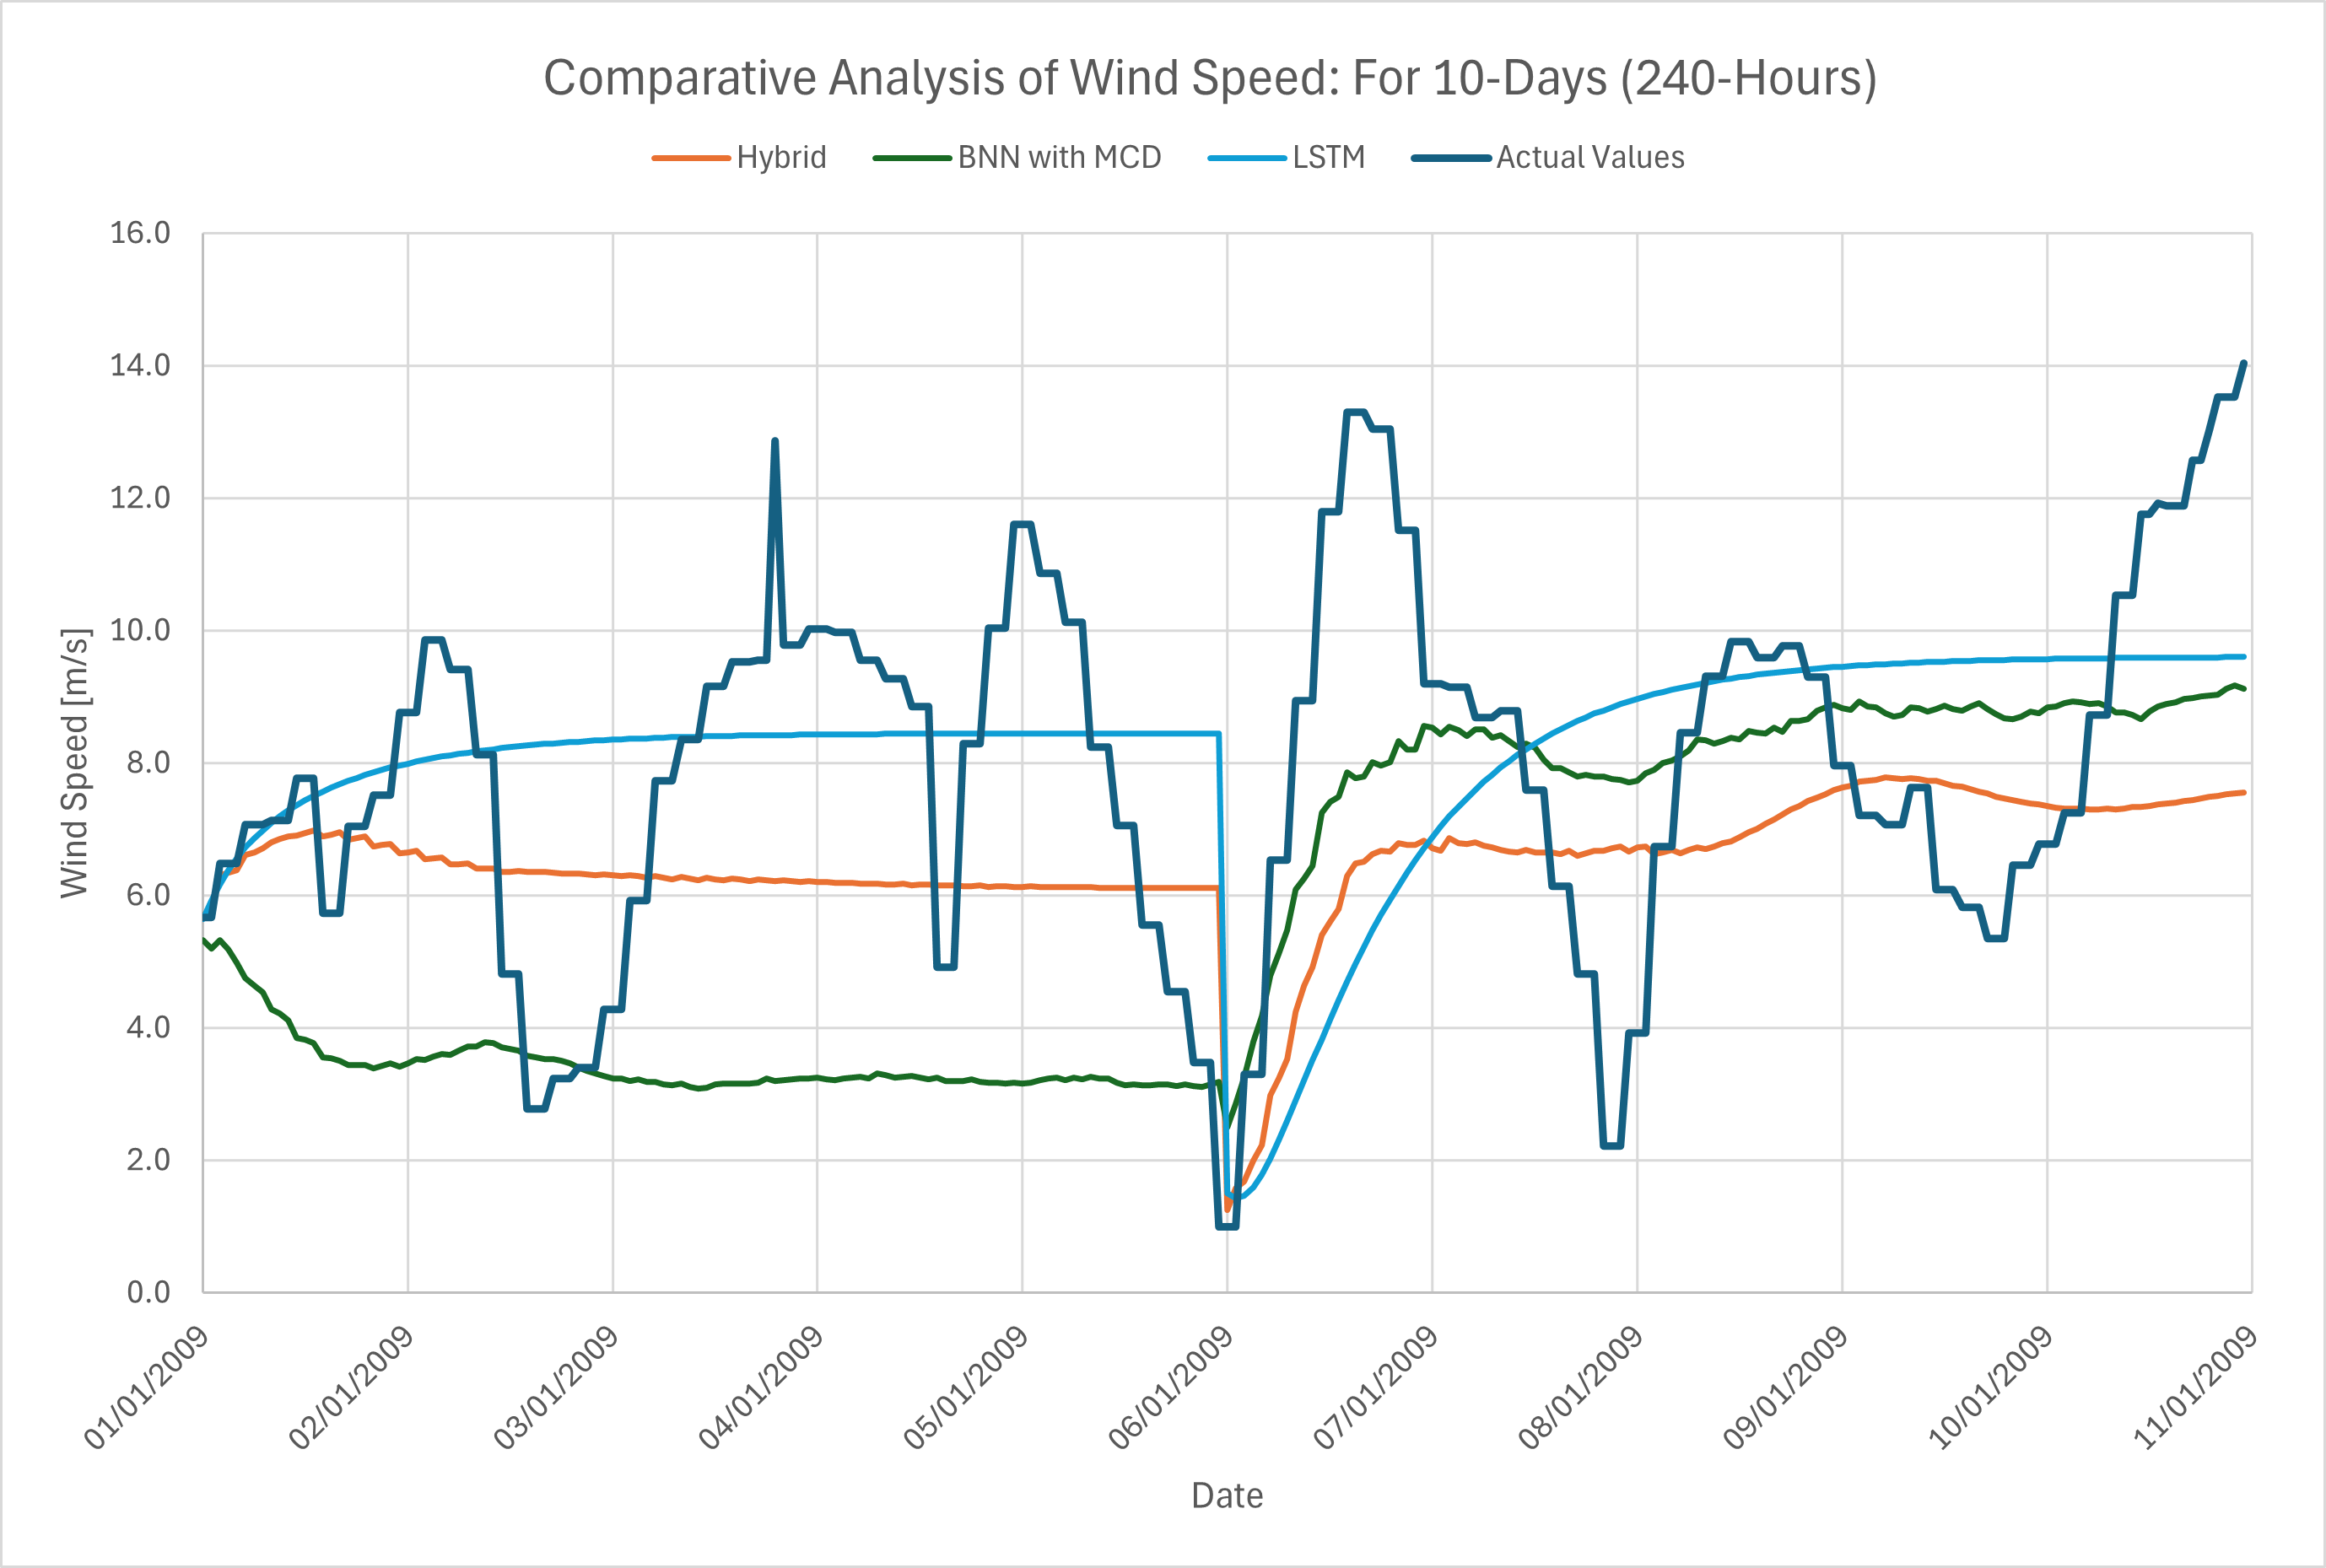
\includegraphics[width=\textwidth]{graphs/wind speed 240 hours.png}
        \caption{Wind Speed}
        \label{fig:wind_speed_all_10Day}
    \end{subfigure}
    \caption{Comparative analyses over the first 10 days (240 hours)}
    \label{fig:combined_10day}
\end{figure}

\noindent To estimate how well the models perform, the residuals are evaluated with a box plot in Figure \ref{fig:combined_box}. These plots show how the residuals of all forecasts are distributed to the actual values. Each box shows the interquartile range (IQR), the horizontal line inside the box is the median, the "x" symbol marks the mean. Whiskers extend to 1.5 times the IQR and individual residuals are shown outside the range.\\

\noindent The Hybrid model has distribution of the residuals that look stable. Although showing a median below zero, suggesting it is underfitting, the spread of the forecasted values is much lower. If looking at the BNN with MCD, the spread in the residuals is much larger, which indicates there is more variability between the residuals. This is not beneficial where the forecast accuracy will go down when this residual spread is higher. The residuals of the LSTM model show somewhat the same range, but there is one significant difference in the outliers. This model has a lot of outliers above the Whisker extend, suggesting there are a lot of forecasted values above the actual values.\\

\begin{figure}[ht!]
    \centering
    \begin{subfigure}[b]{0.49\textwidth}
        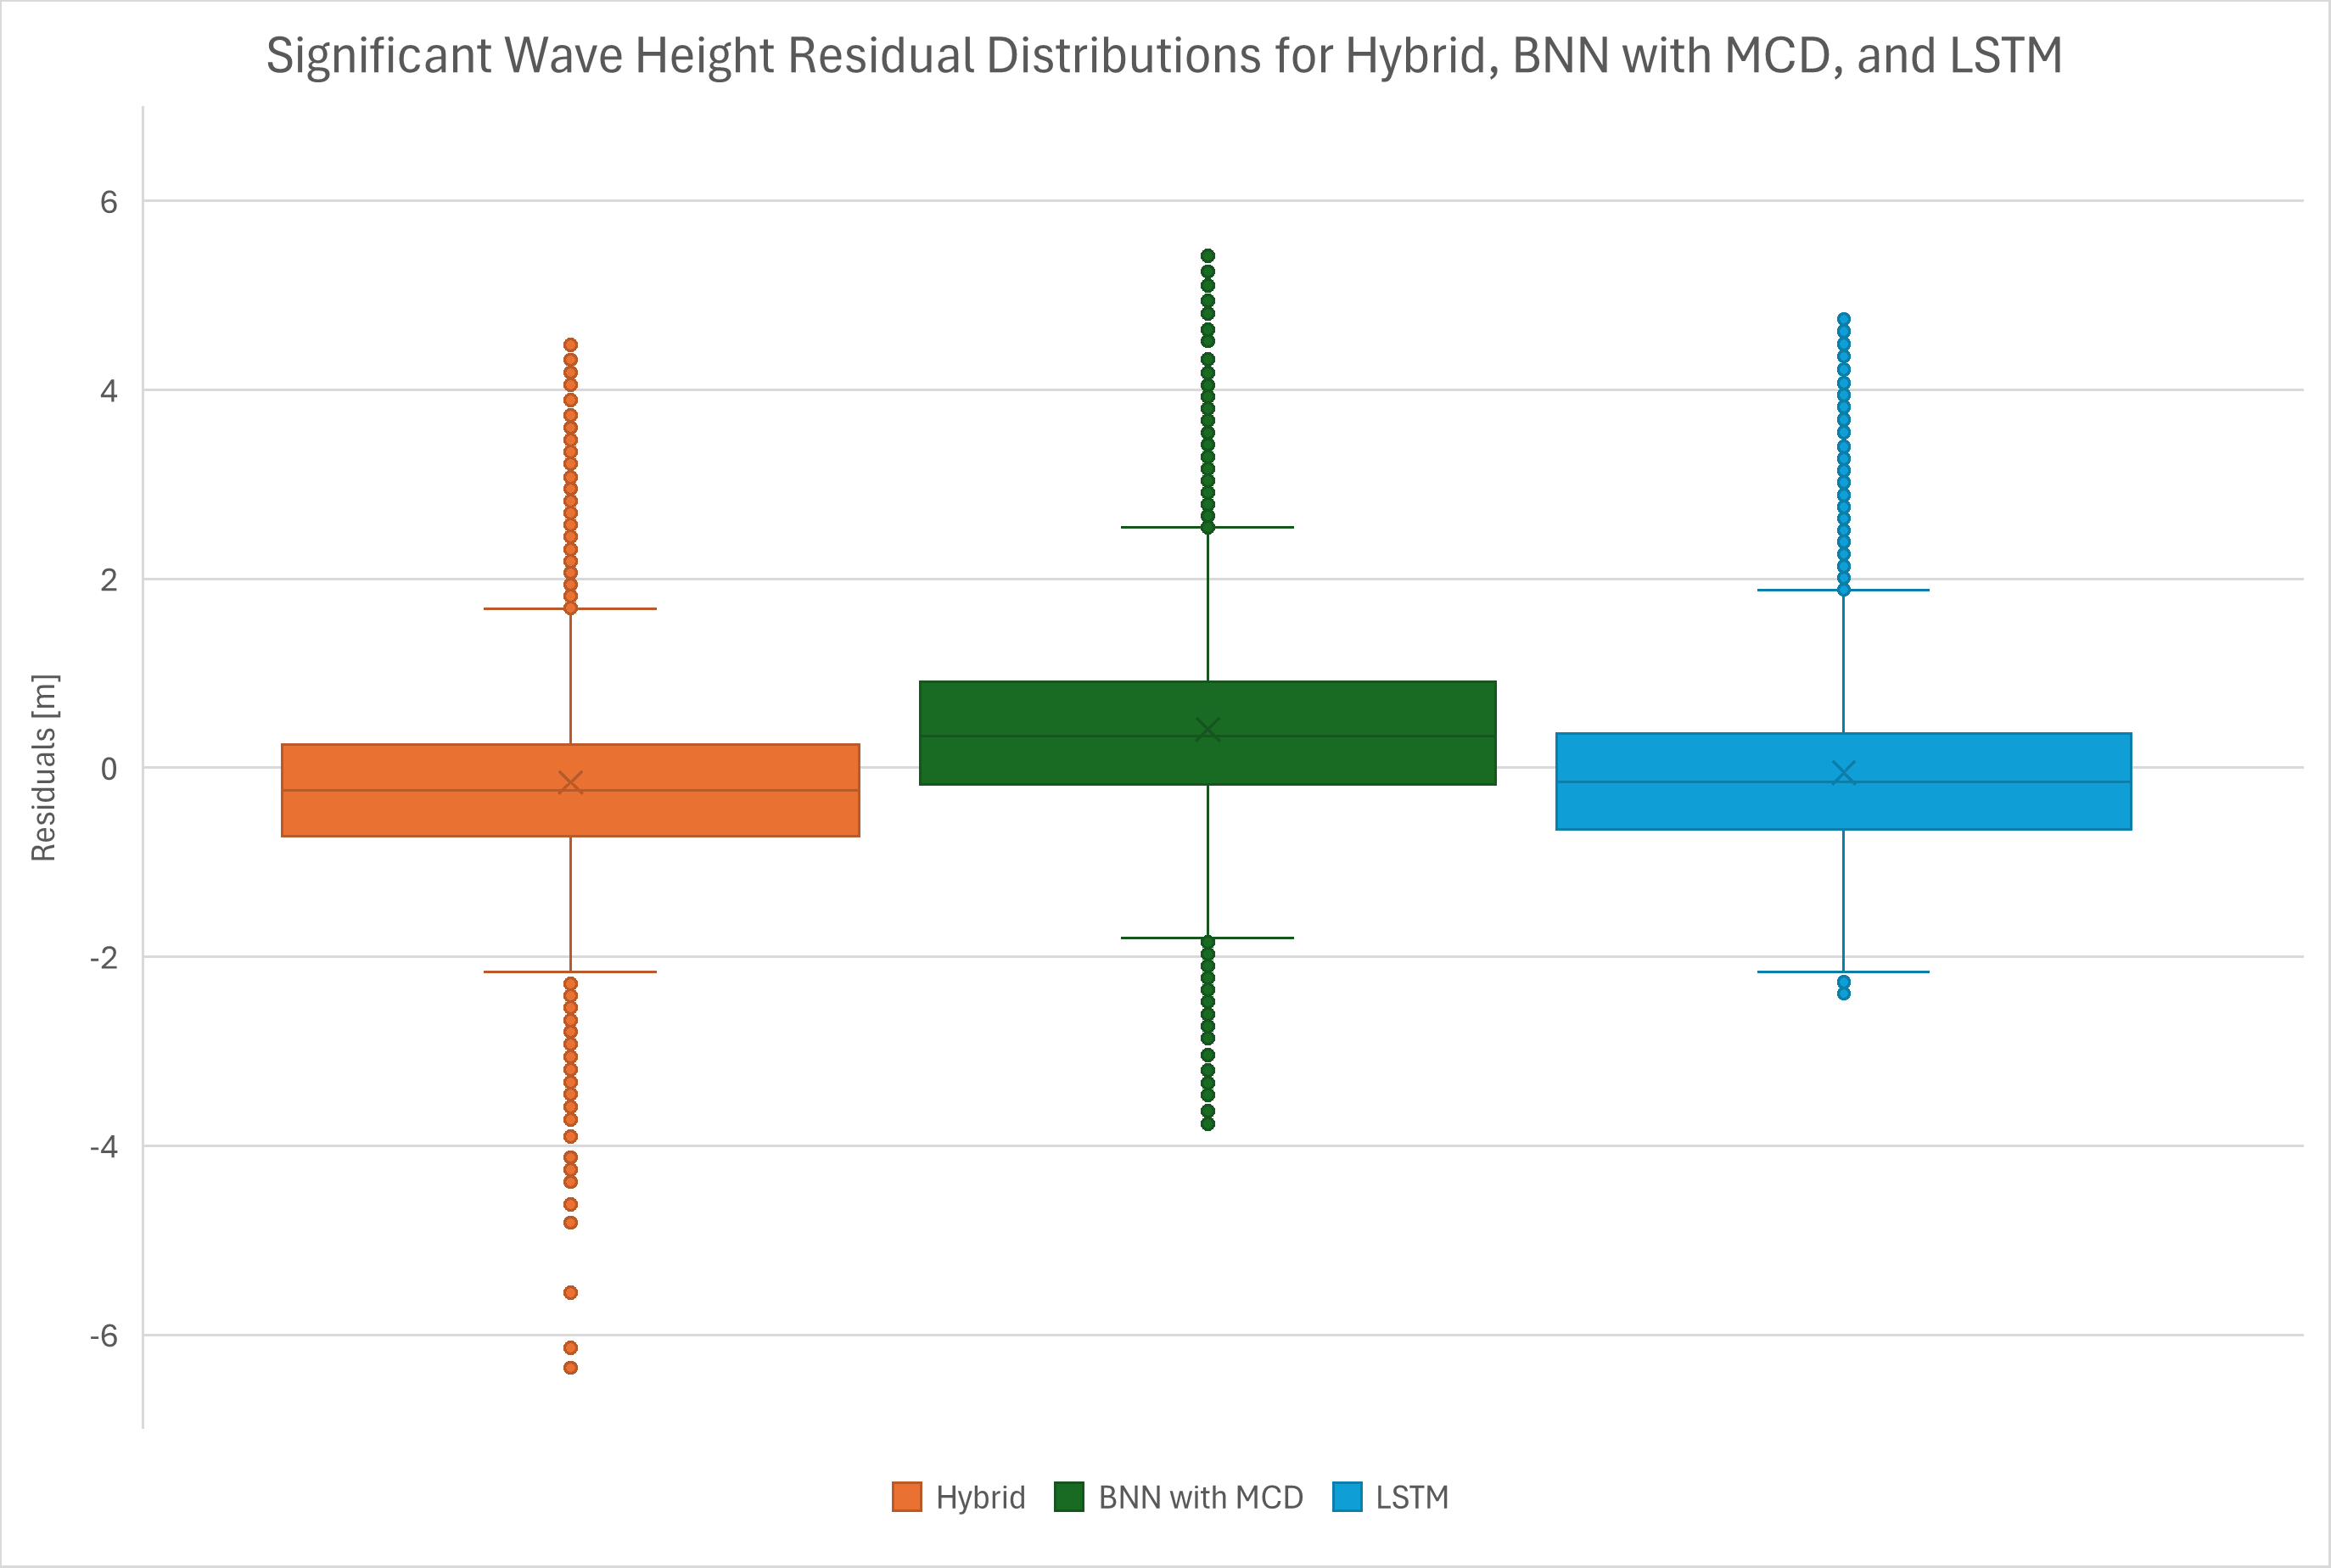
\includegraphics[width=\textwidth]{graphs/Box s_wht.png}
        \caption{Significant Wave Height}
        \label{fig:s_wht_box}
    \end{subfigure}
    \hfill
    \begin{subfigure}[b]{0.49\textwidth}
        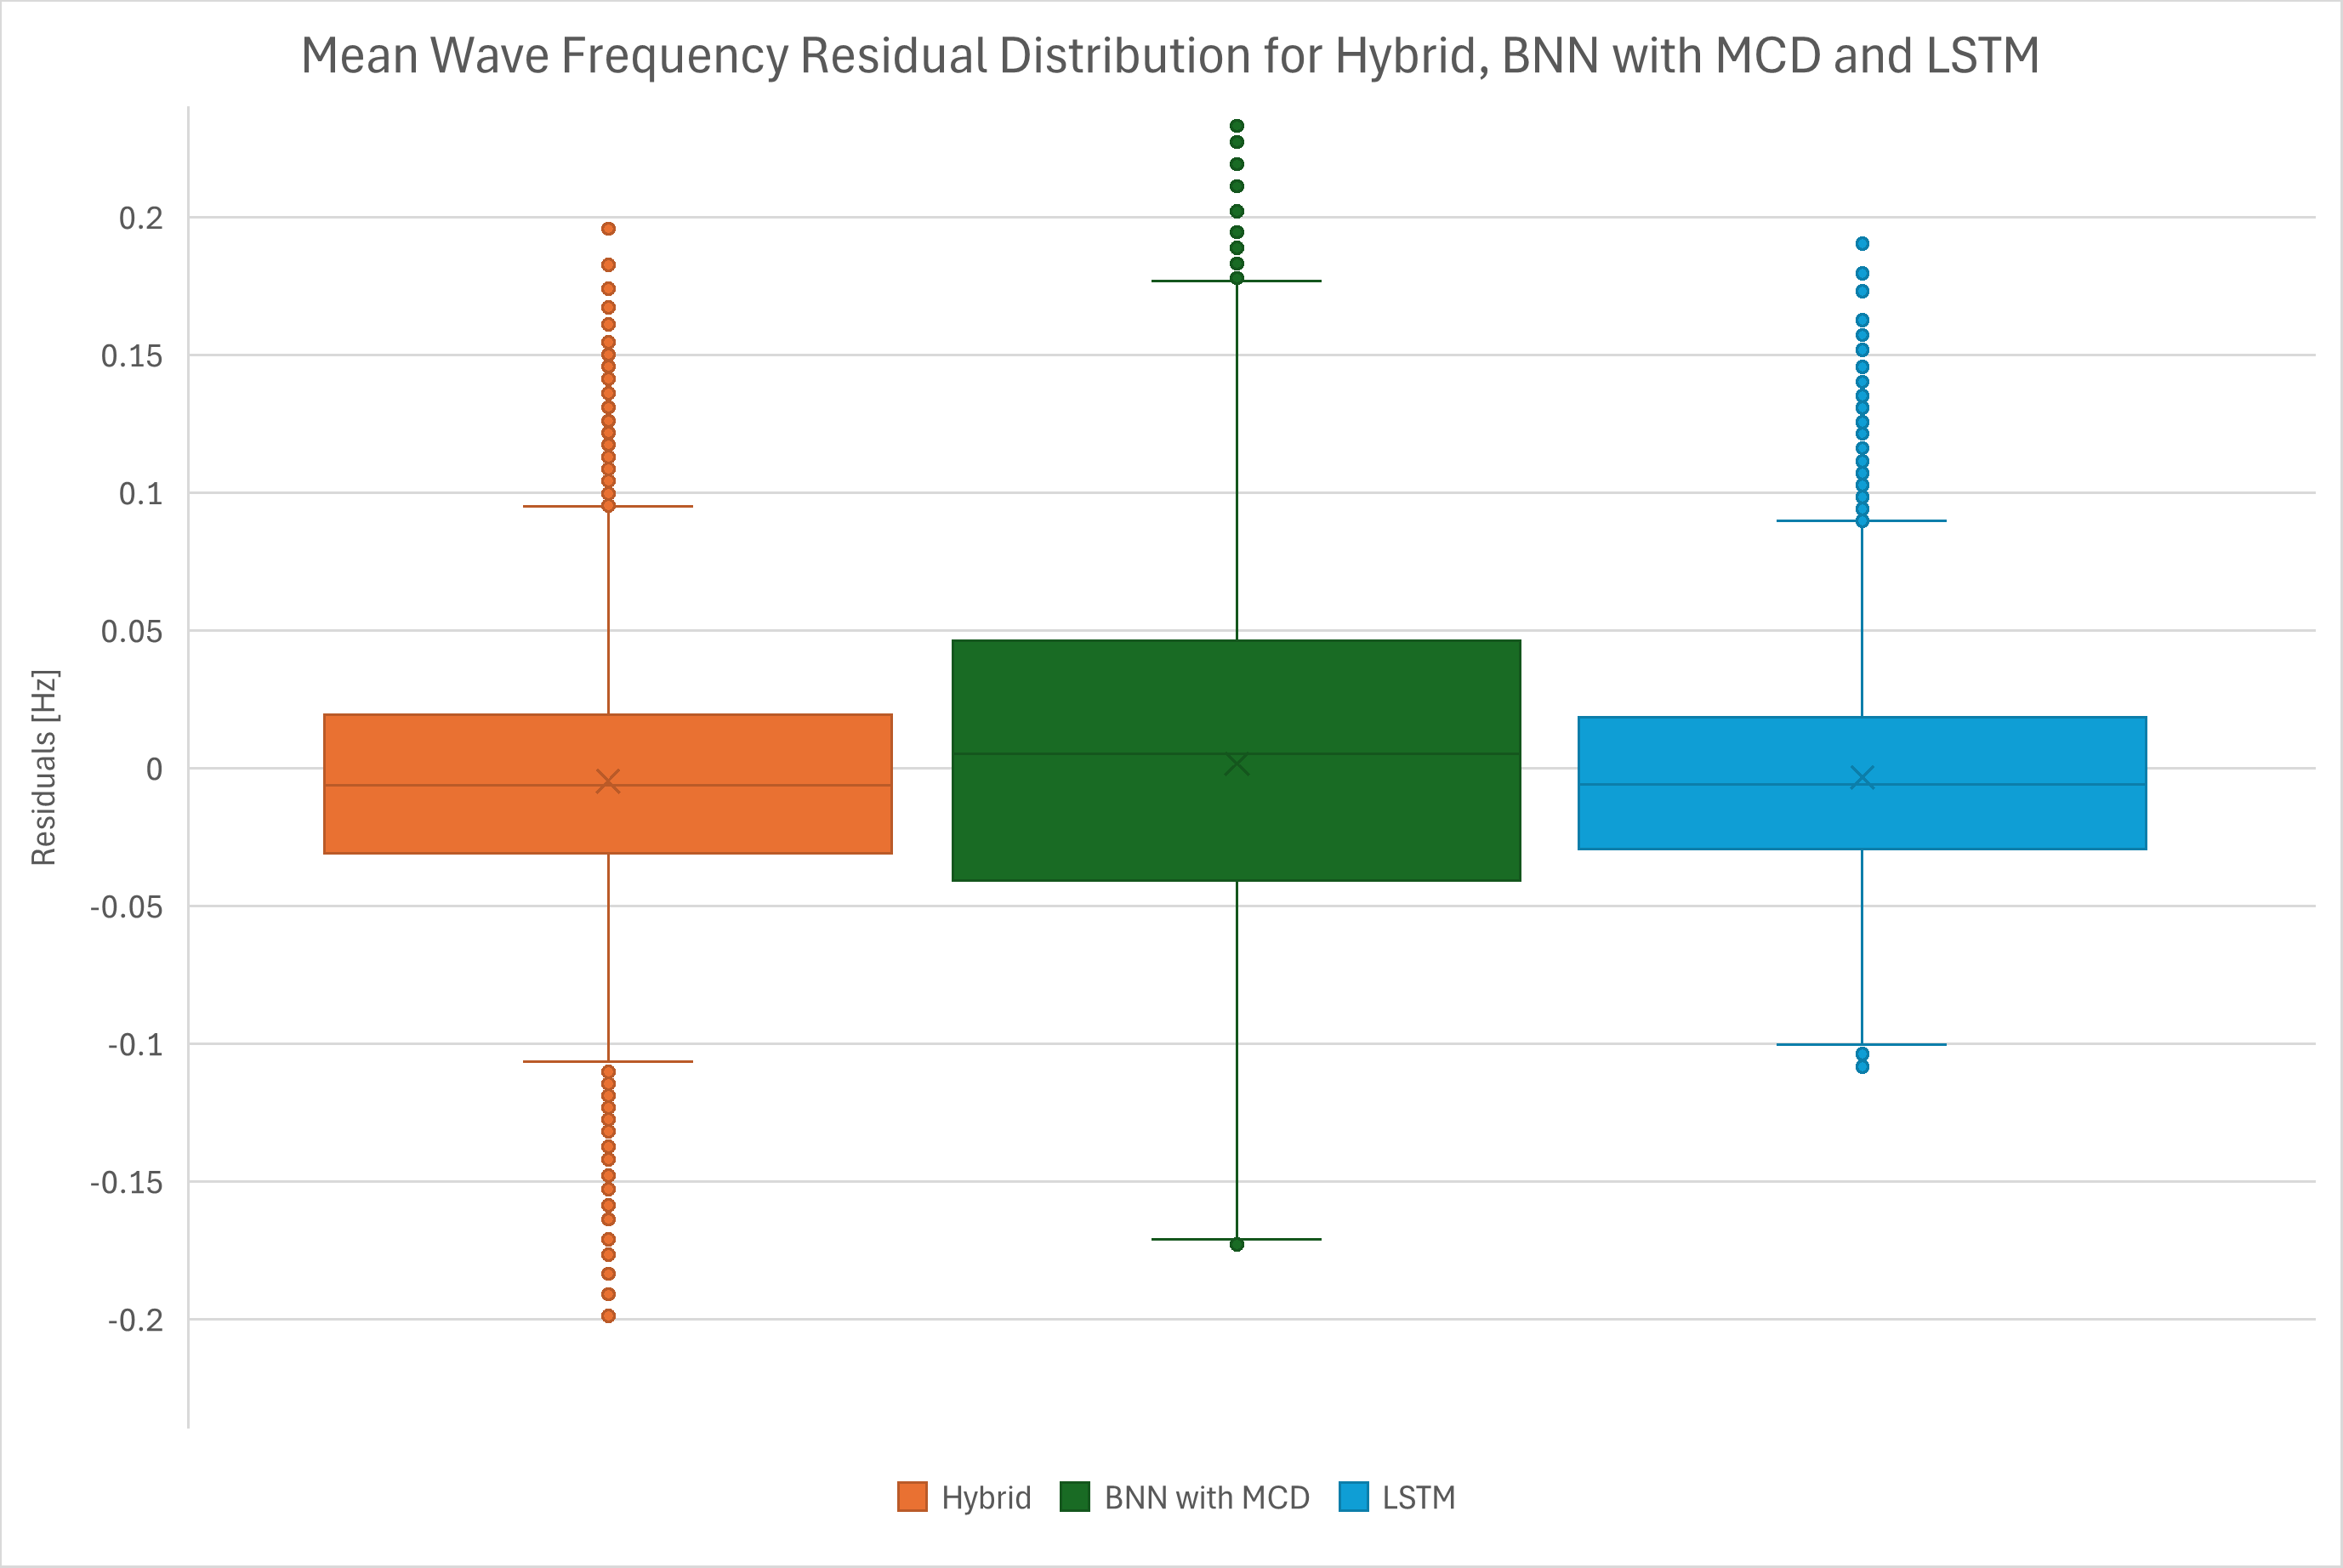
\includegraphics[width=\textwidth]{graphs/Box mean_fr.png}
        \caption{Mean Wave Frequency}
        \label{fig:mean_fr_box}
    \end{subfigure}
    \vskip\baselineskip
    \begin{subfigure}[b]{0.49\textwidth}
        \centering
        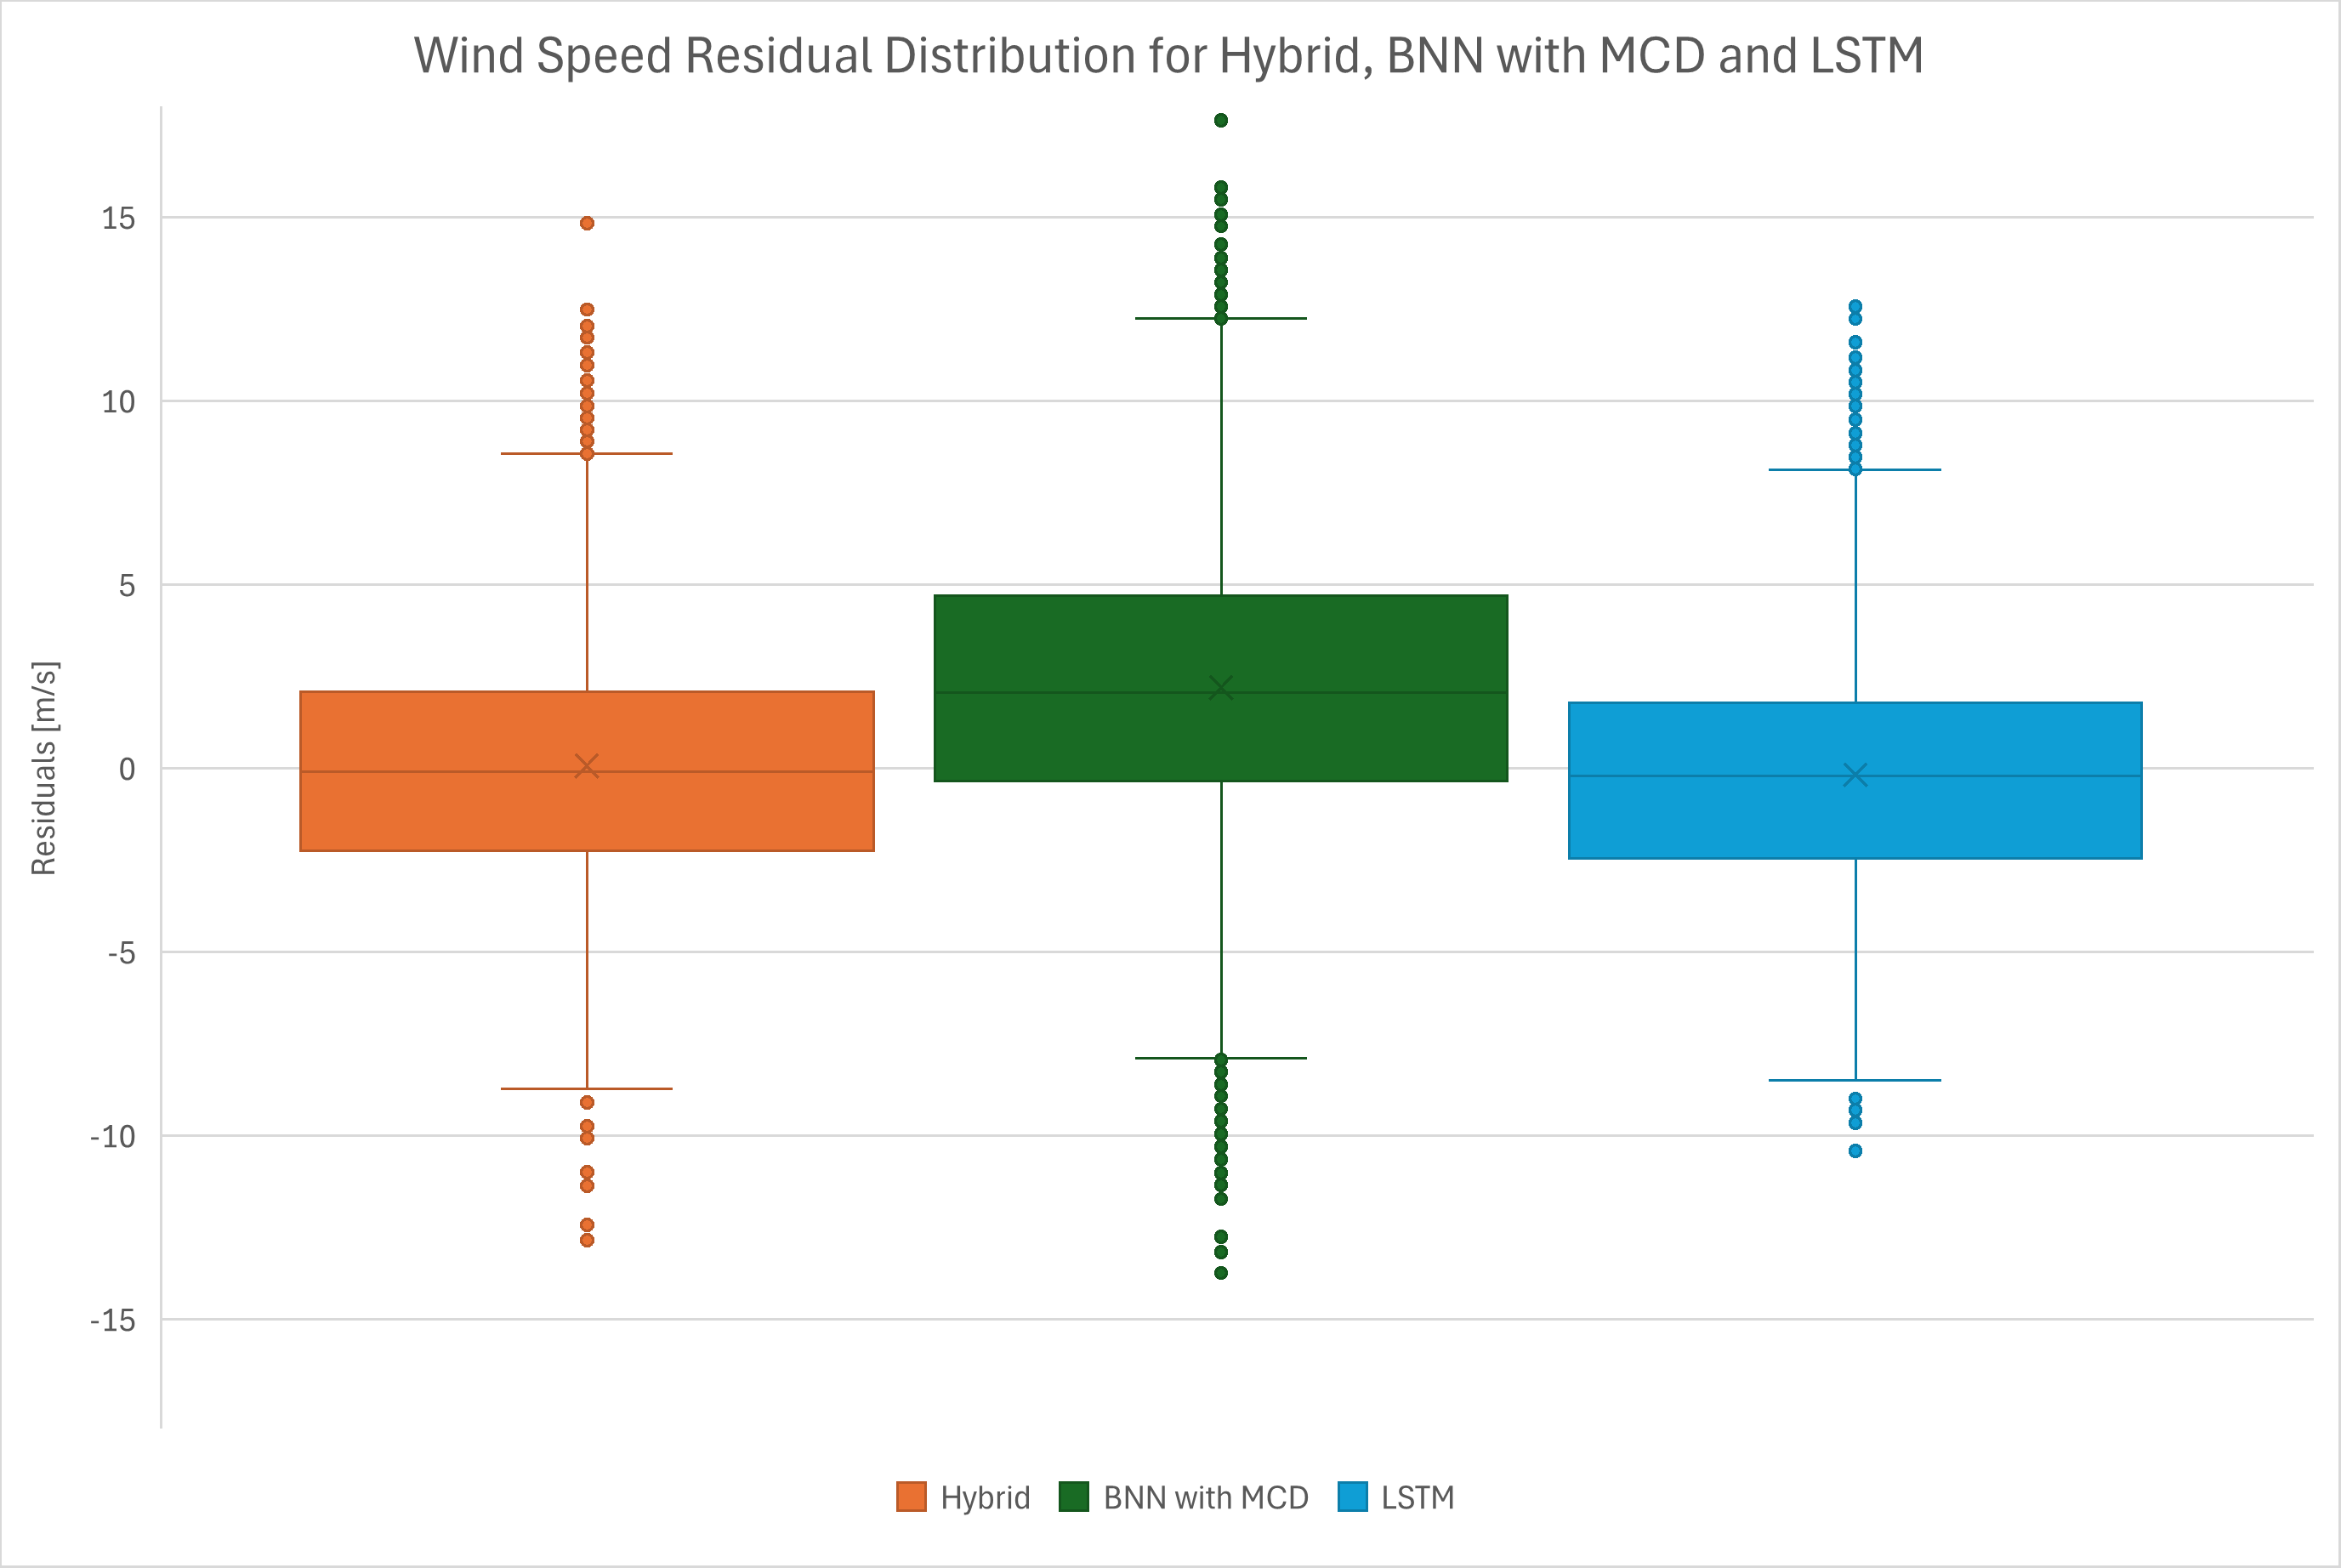
\includegraphics[width=\textwidth]{graphs/Box wind_speed.png}
        \caption{Wind Speed}
        \label{fig:wind_speed_box}
    \end{subfigure}
    \caption{Comparative box plot of significant wave height, mean wave frequency, and wind speed}
    \label{fig:combined_box}
\end{figure}

\noindent Overall, the comparative results indicate the three models are capturing the overall trends; how they do so differs a lot. The forecasted values plotted against the actual values, the residuals plot and a scatter plot of each model can be found in Appendix \ref{results all models 5 days}. The LSTM model shows exponential tendencies as visible in Figure \ref{fig:s_wht_all_10Day}. The BNN with MCD shows greater variability in the box plots, which is not beneficial when an accurate forecast is necessary. The Hybrid model shows consistent forecasts with a low error and its residuals tend to stay closer to the mean. These reasons to further analyse the Hybrid ARIMA-ANN model.

\newpage

\section{Hybrid Model Results}
\label{hybrid_model_results}
This section will investigate the sensitivity of the Hybrid model with the usage of different refit intervals, these are: 6 hours, 12 hours, 1 day, 2 days, 3 days, 4 days, 5 days, 6 days, 7 days, 2 weeks, 4 weeks. The forecasted values against the actual values, the residuals plot and the scatter plots for each refit interval can be seen in Appendix \ref{results hybrid different refit}.\\

\noindent While there are a lot of different outcomes for the evaluation metrics: MSE, MAE, RMSE and $R^2$ will be evaluated with the graphs in Figure \ref{fig:hybrid_refit_metrics}. The left y-axis is used for the MSE, MAE and RMSE, and the right y-axis showcases the $R^2$ values. The x-axis is not equally weighted, so the distance between 0.25 and 0.5 days is the same as the distance between 7 days and 14 days. For the significant wave height in Figure \ref{fig:s_wht_refit} and the mean wave frequency in Figure \ref{fig:mean_fr_refit}, it can be seen that the curves steadily increase for the MSE, MAE, and RMSE over time. Another thing visible is that around the 3-day refit interval rate the $R^2$ drops below zero, indicating the model is outperformed by a naive baseline. For the wind speed in Figure \ref{fig:wind_speed_refit} the errors increase much less drastically and seem to move towards a maximum value over time. Also, the $R^2$ only drops below zero after around a 5 day interval, all indicating the model performs best on this parameter. Overall longer refit intervals lead to higher values of MSE, MAE and RMSE and lower values for $R^2$

\begin{figure}[ht!]
    \centering
    \begin{subfigure}[b]{0.49\textwidth}
        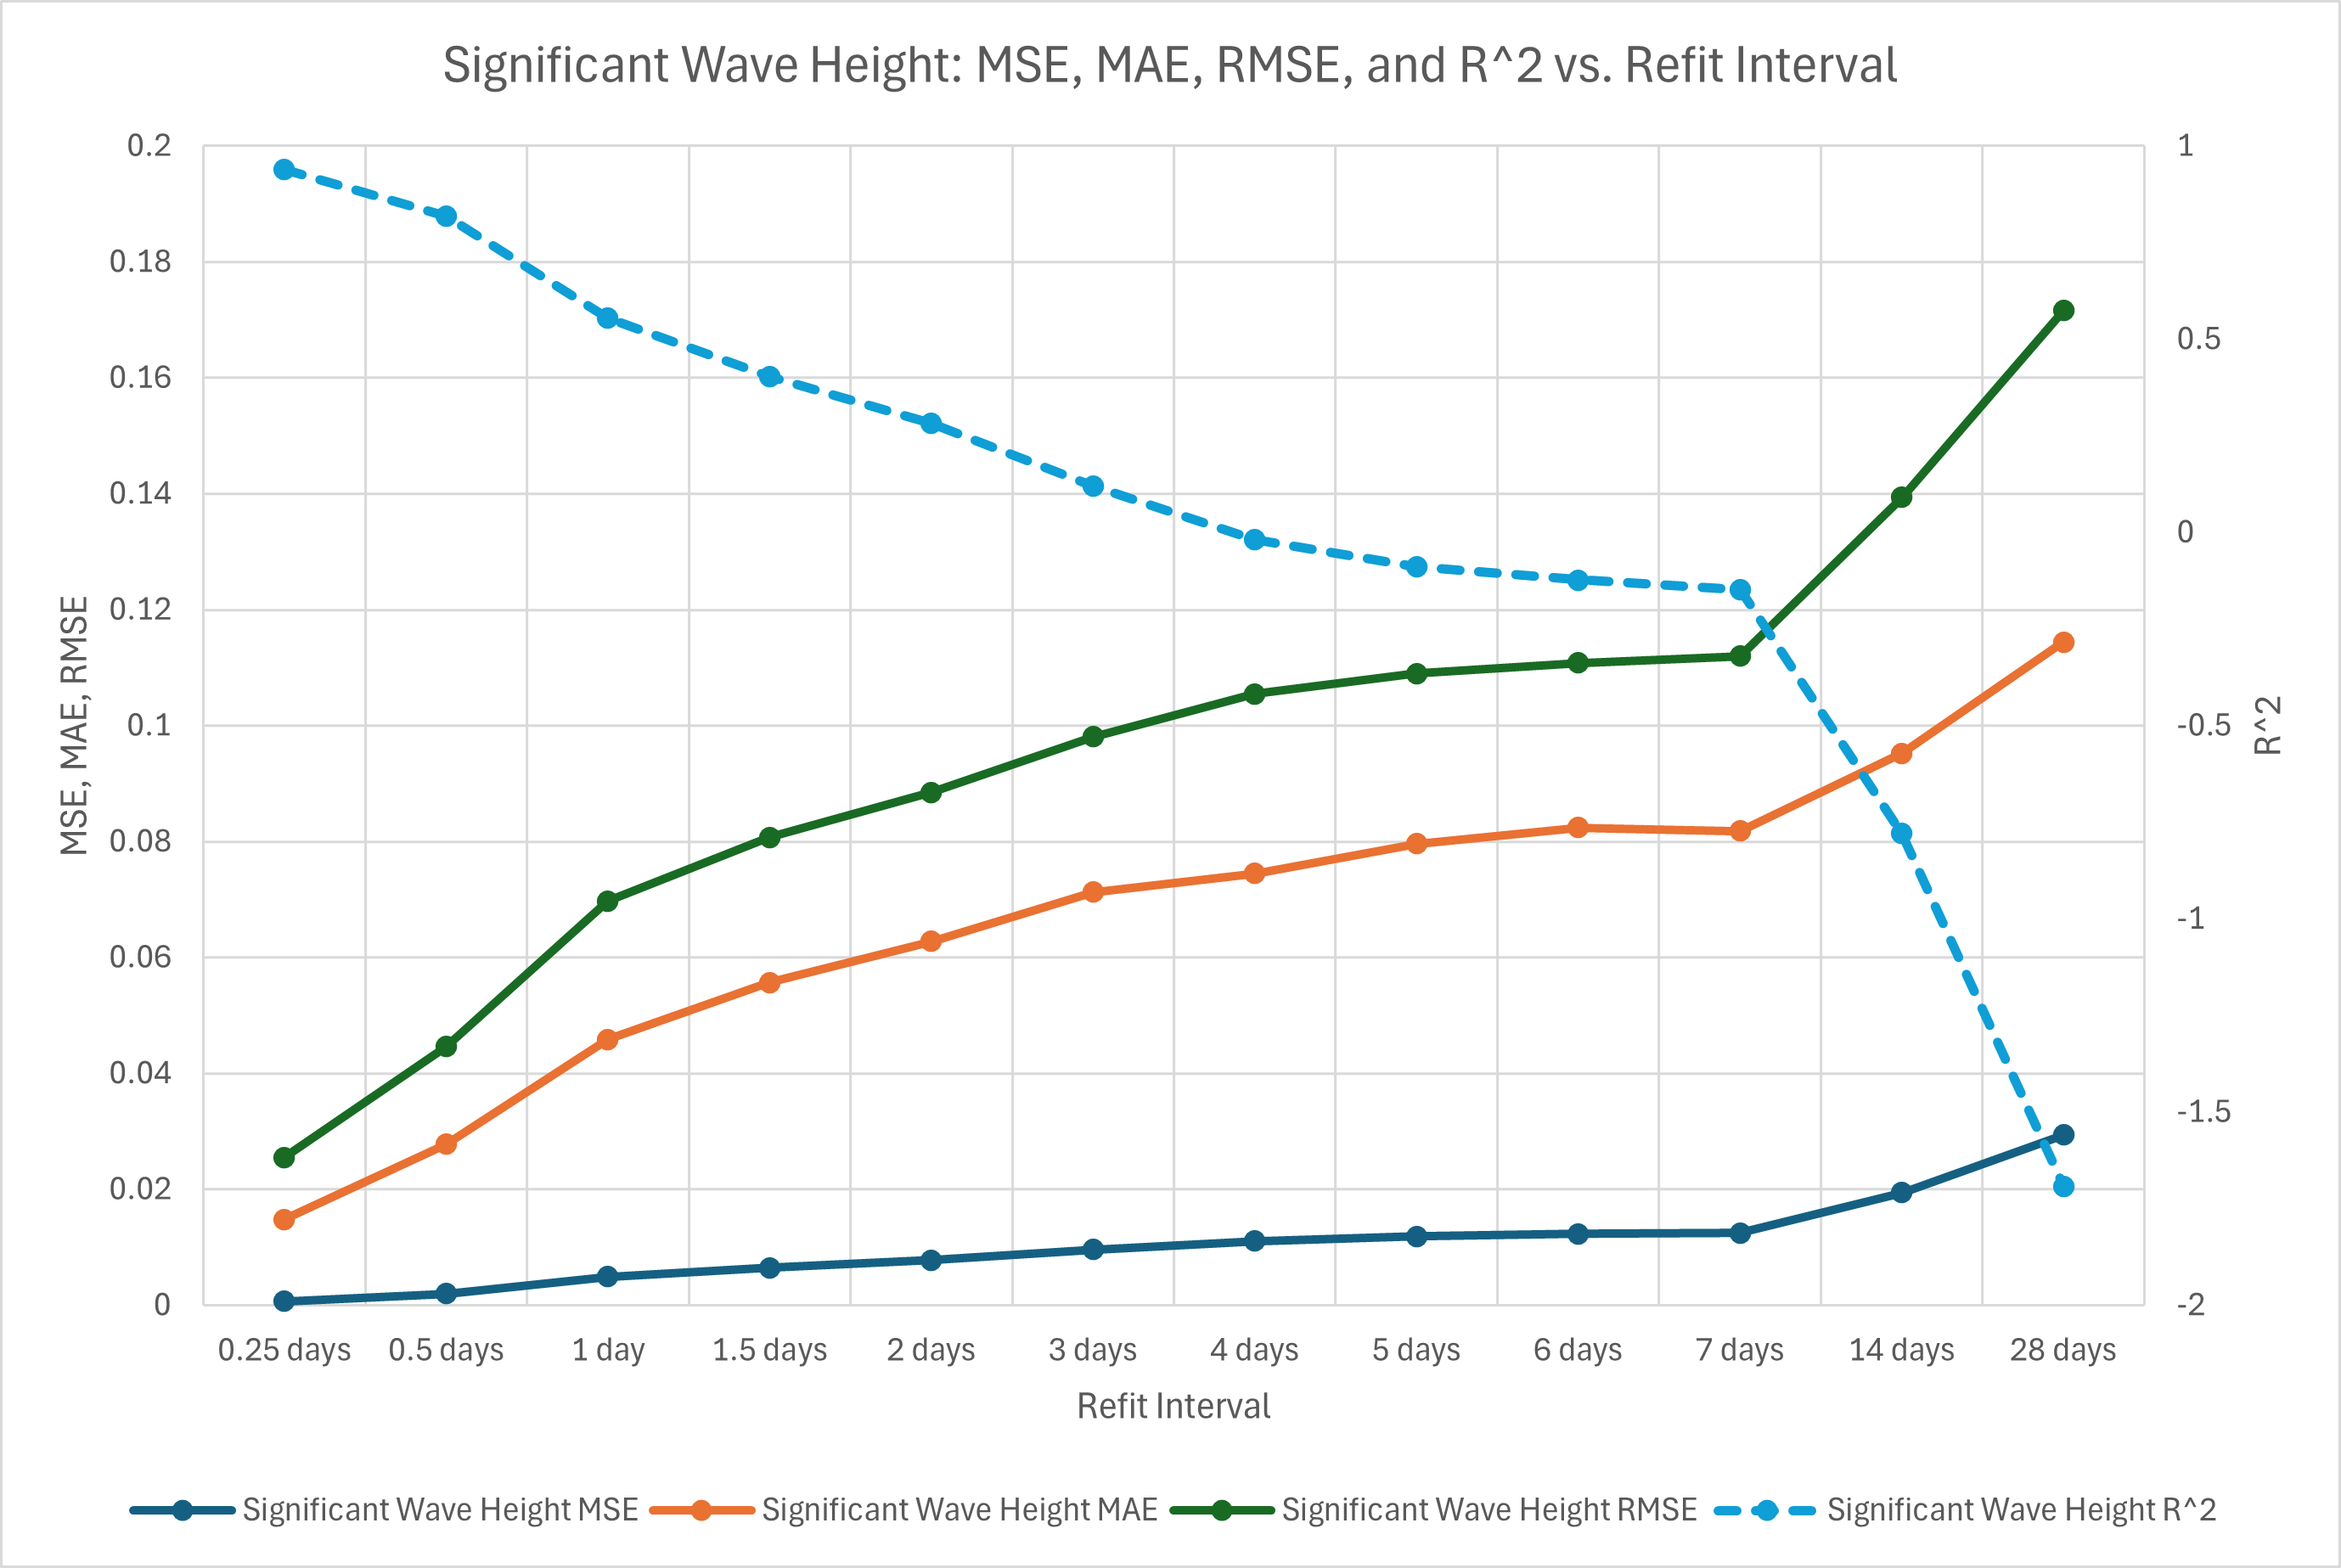
\includegraphics[width=\textwidth]{graphs/Refit_s_wht_metrics.png}
        \caption{Significant Wave Height}
        \label{fig:s_wht_refit}
    \end{subfigure}
    \hfill
    \begin{subfigure}[b]{0.49\textwidth}
        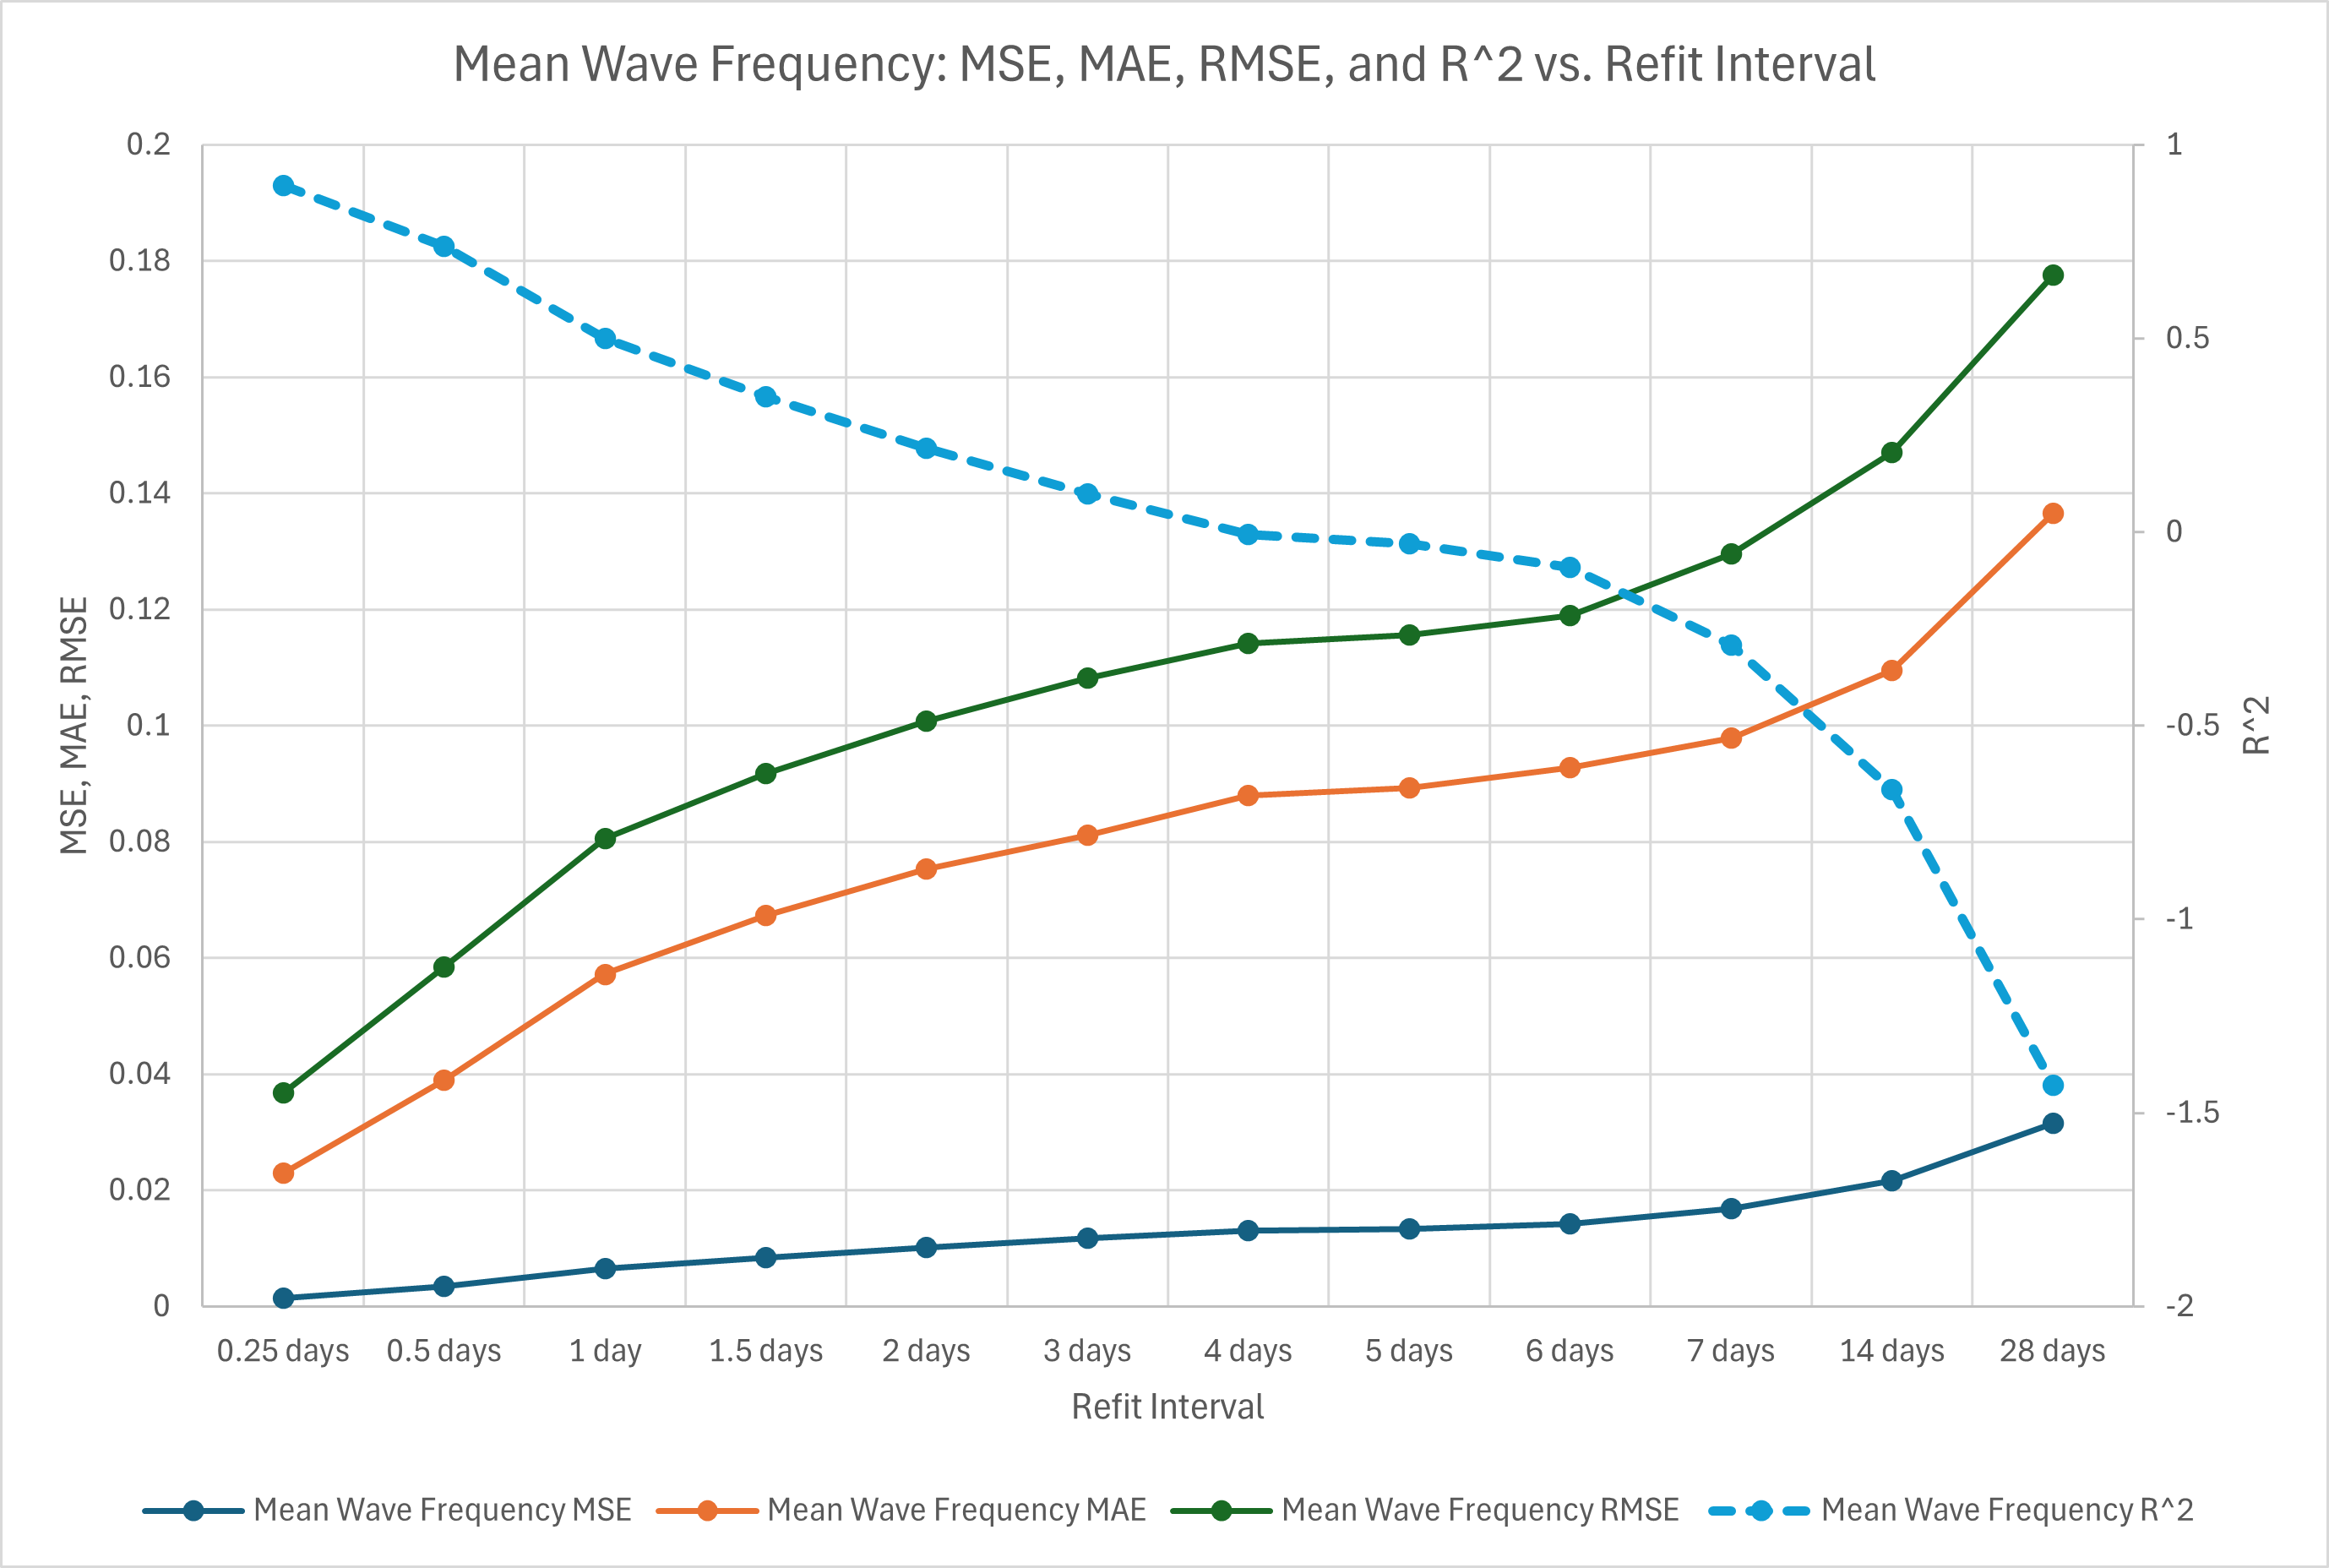
\includegraphics[width=\textwidth]{graphs/Refit_mean_fr_metrics.png}
        \caption{Mean Wave Frequency}
        \label{fig:mean_fr_refit}
    \end{subfigure}
    \vskip\baselineskip
    \begin{subfigure}[b]{0.49\textwidth}
        \centering
        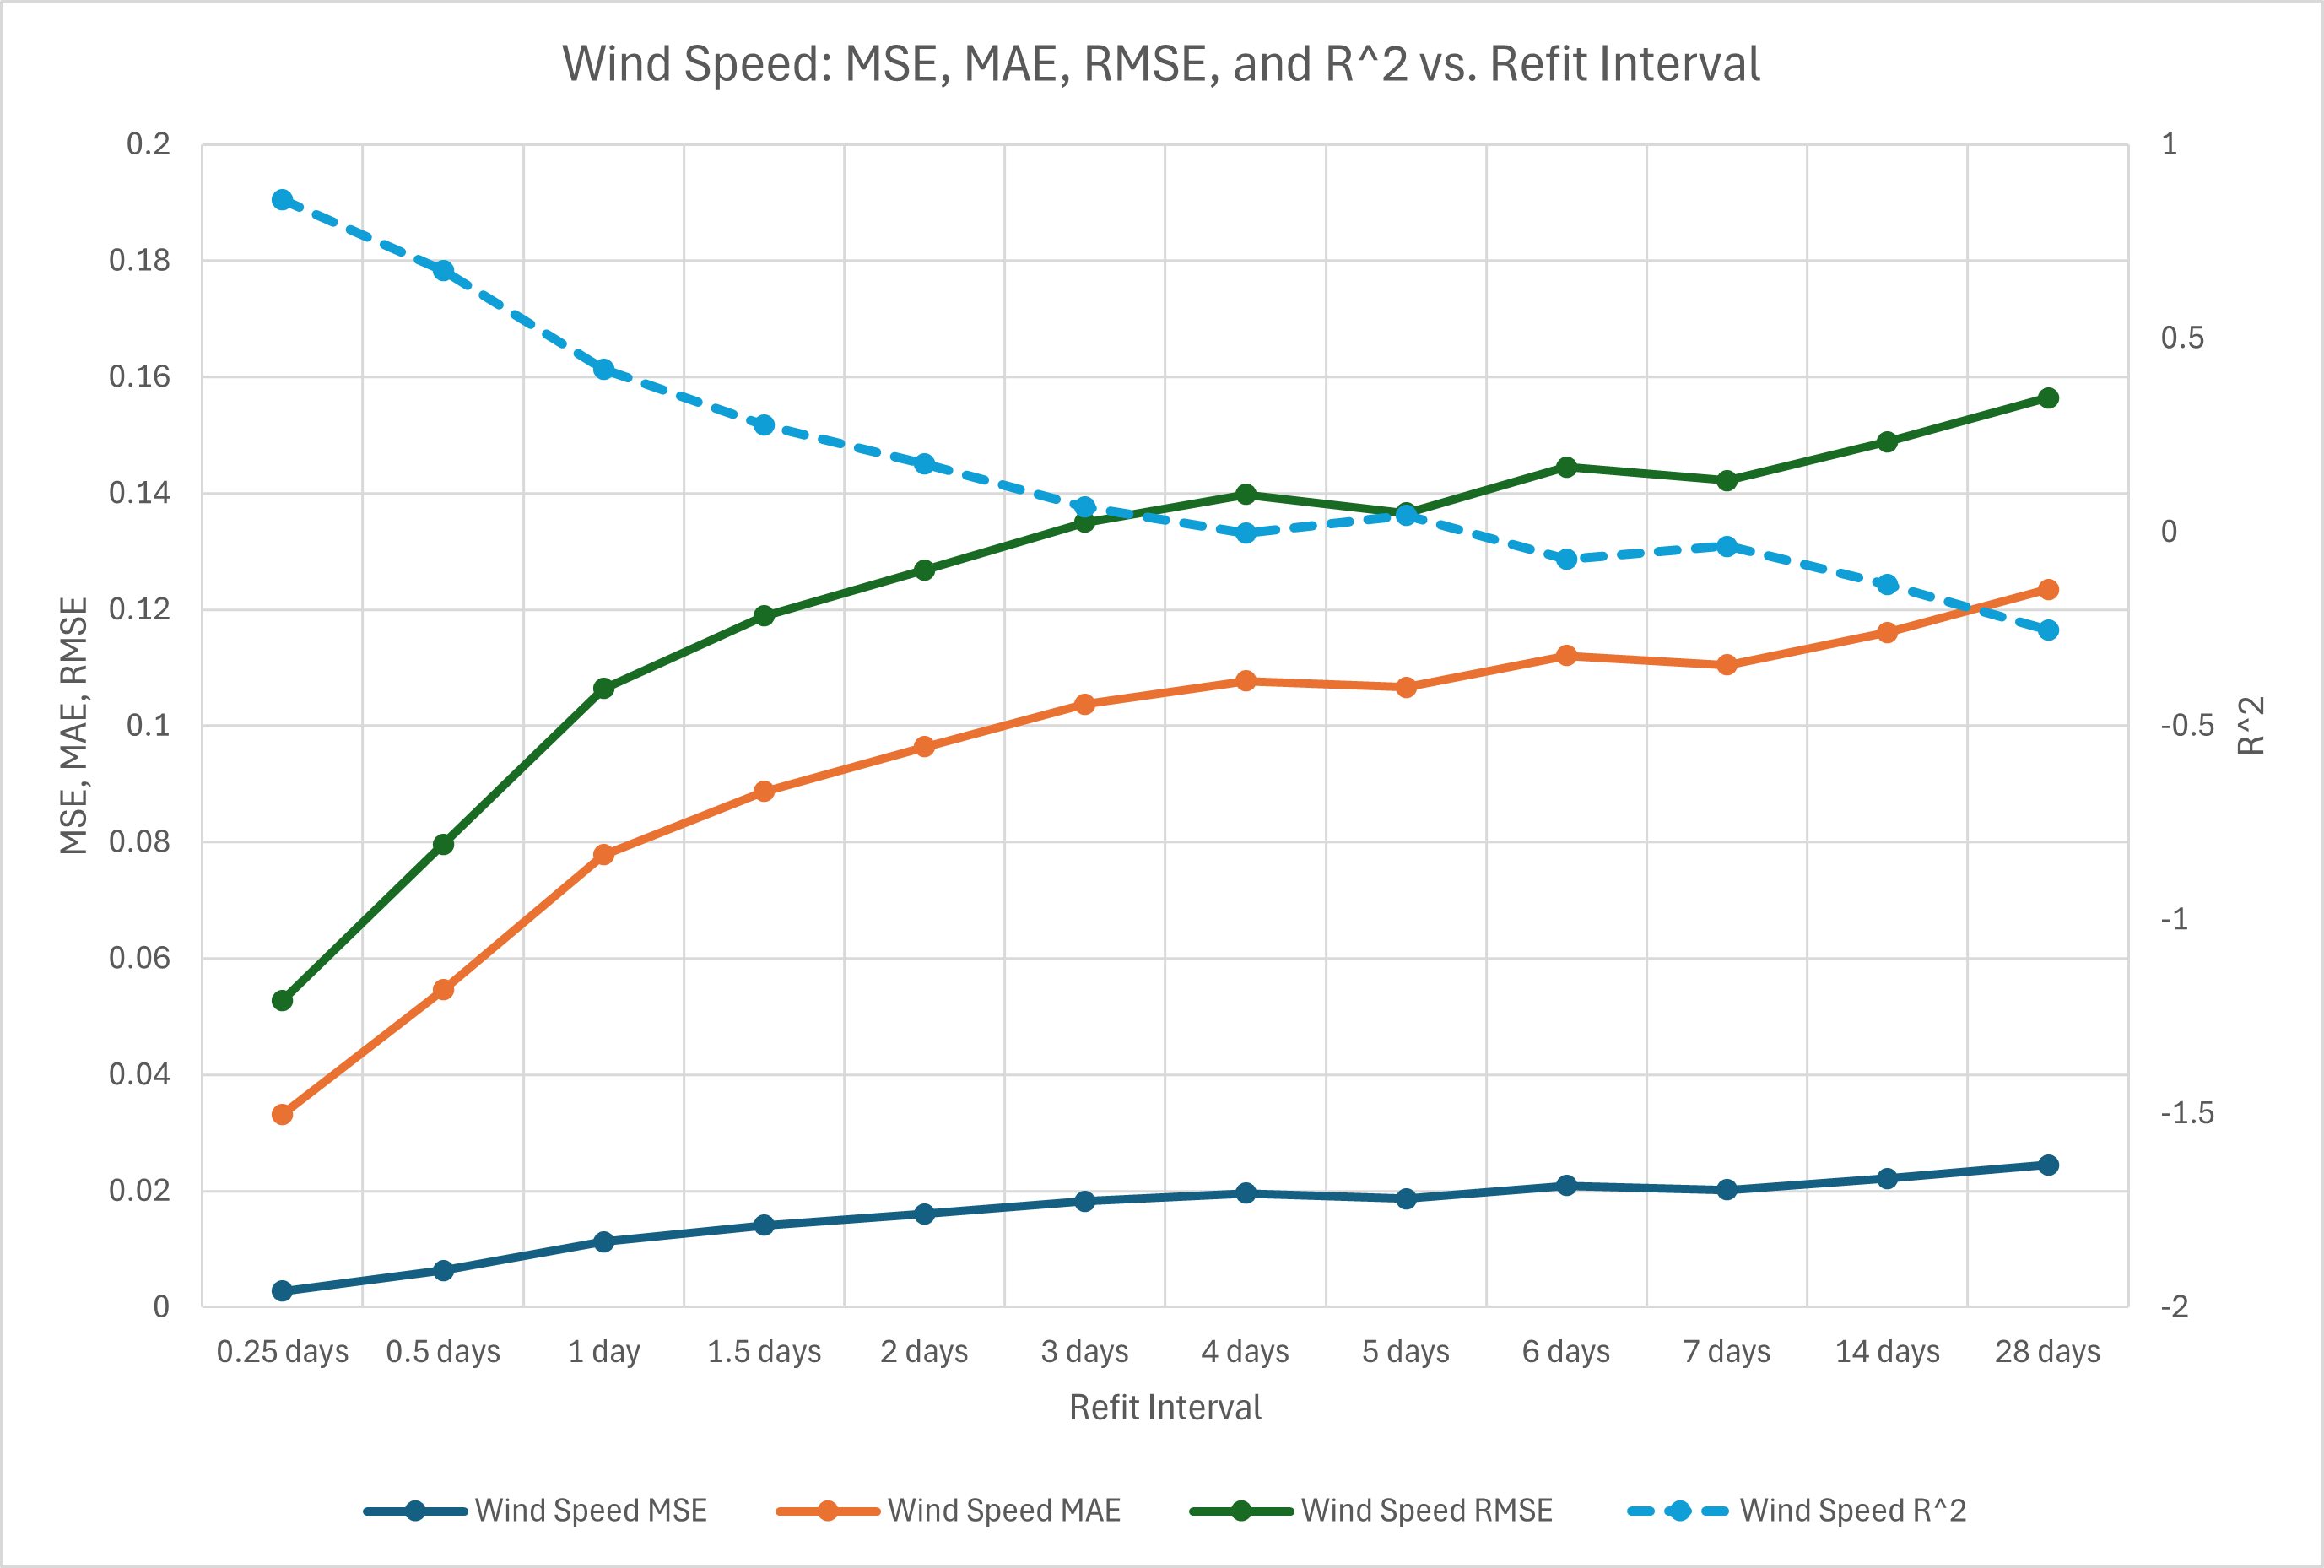
\includegraphics[width=\textwidth]{graphs/Refit_wind_speed_metrics.png}
        \caption{Wind Speed}
        \label{fig:wind_speed_refit}
    \end{subfigure}
    \caption{Line Plots of the Hybrid ARIMA–ANN model’s performance metrics ( MSE, MAE, RMSE, $R^{2}$) under varying refit intervals.}
    \label{fig:hybrid_refit_metrics}
\end{figure}

\newpage

\noindent Below in Figure \ref{fig:hybrid_refit_box}, each box presents the distribution of the residuals for each refit interval in the same way as in Figure \ref{fig:combined_box}. Again it is visible that a longer refit interval leads for all parameters to a larger deviation in the residual errors. The median and mean are in all cases around zero, which indicates the model has the error on average around zero. The model shows, for larger refit intervals, more residuals which fall outside the Whiskers extend. Especially for the values below zero, it is visible that there is a larger error, this indicates that the forecasted value is much larger than the actual value. 

\begin{figure}[ht!]
    \centering
    \begin{subfigure}[b]{0.49\textwidth}
        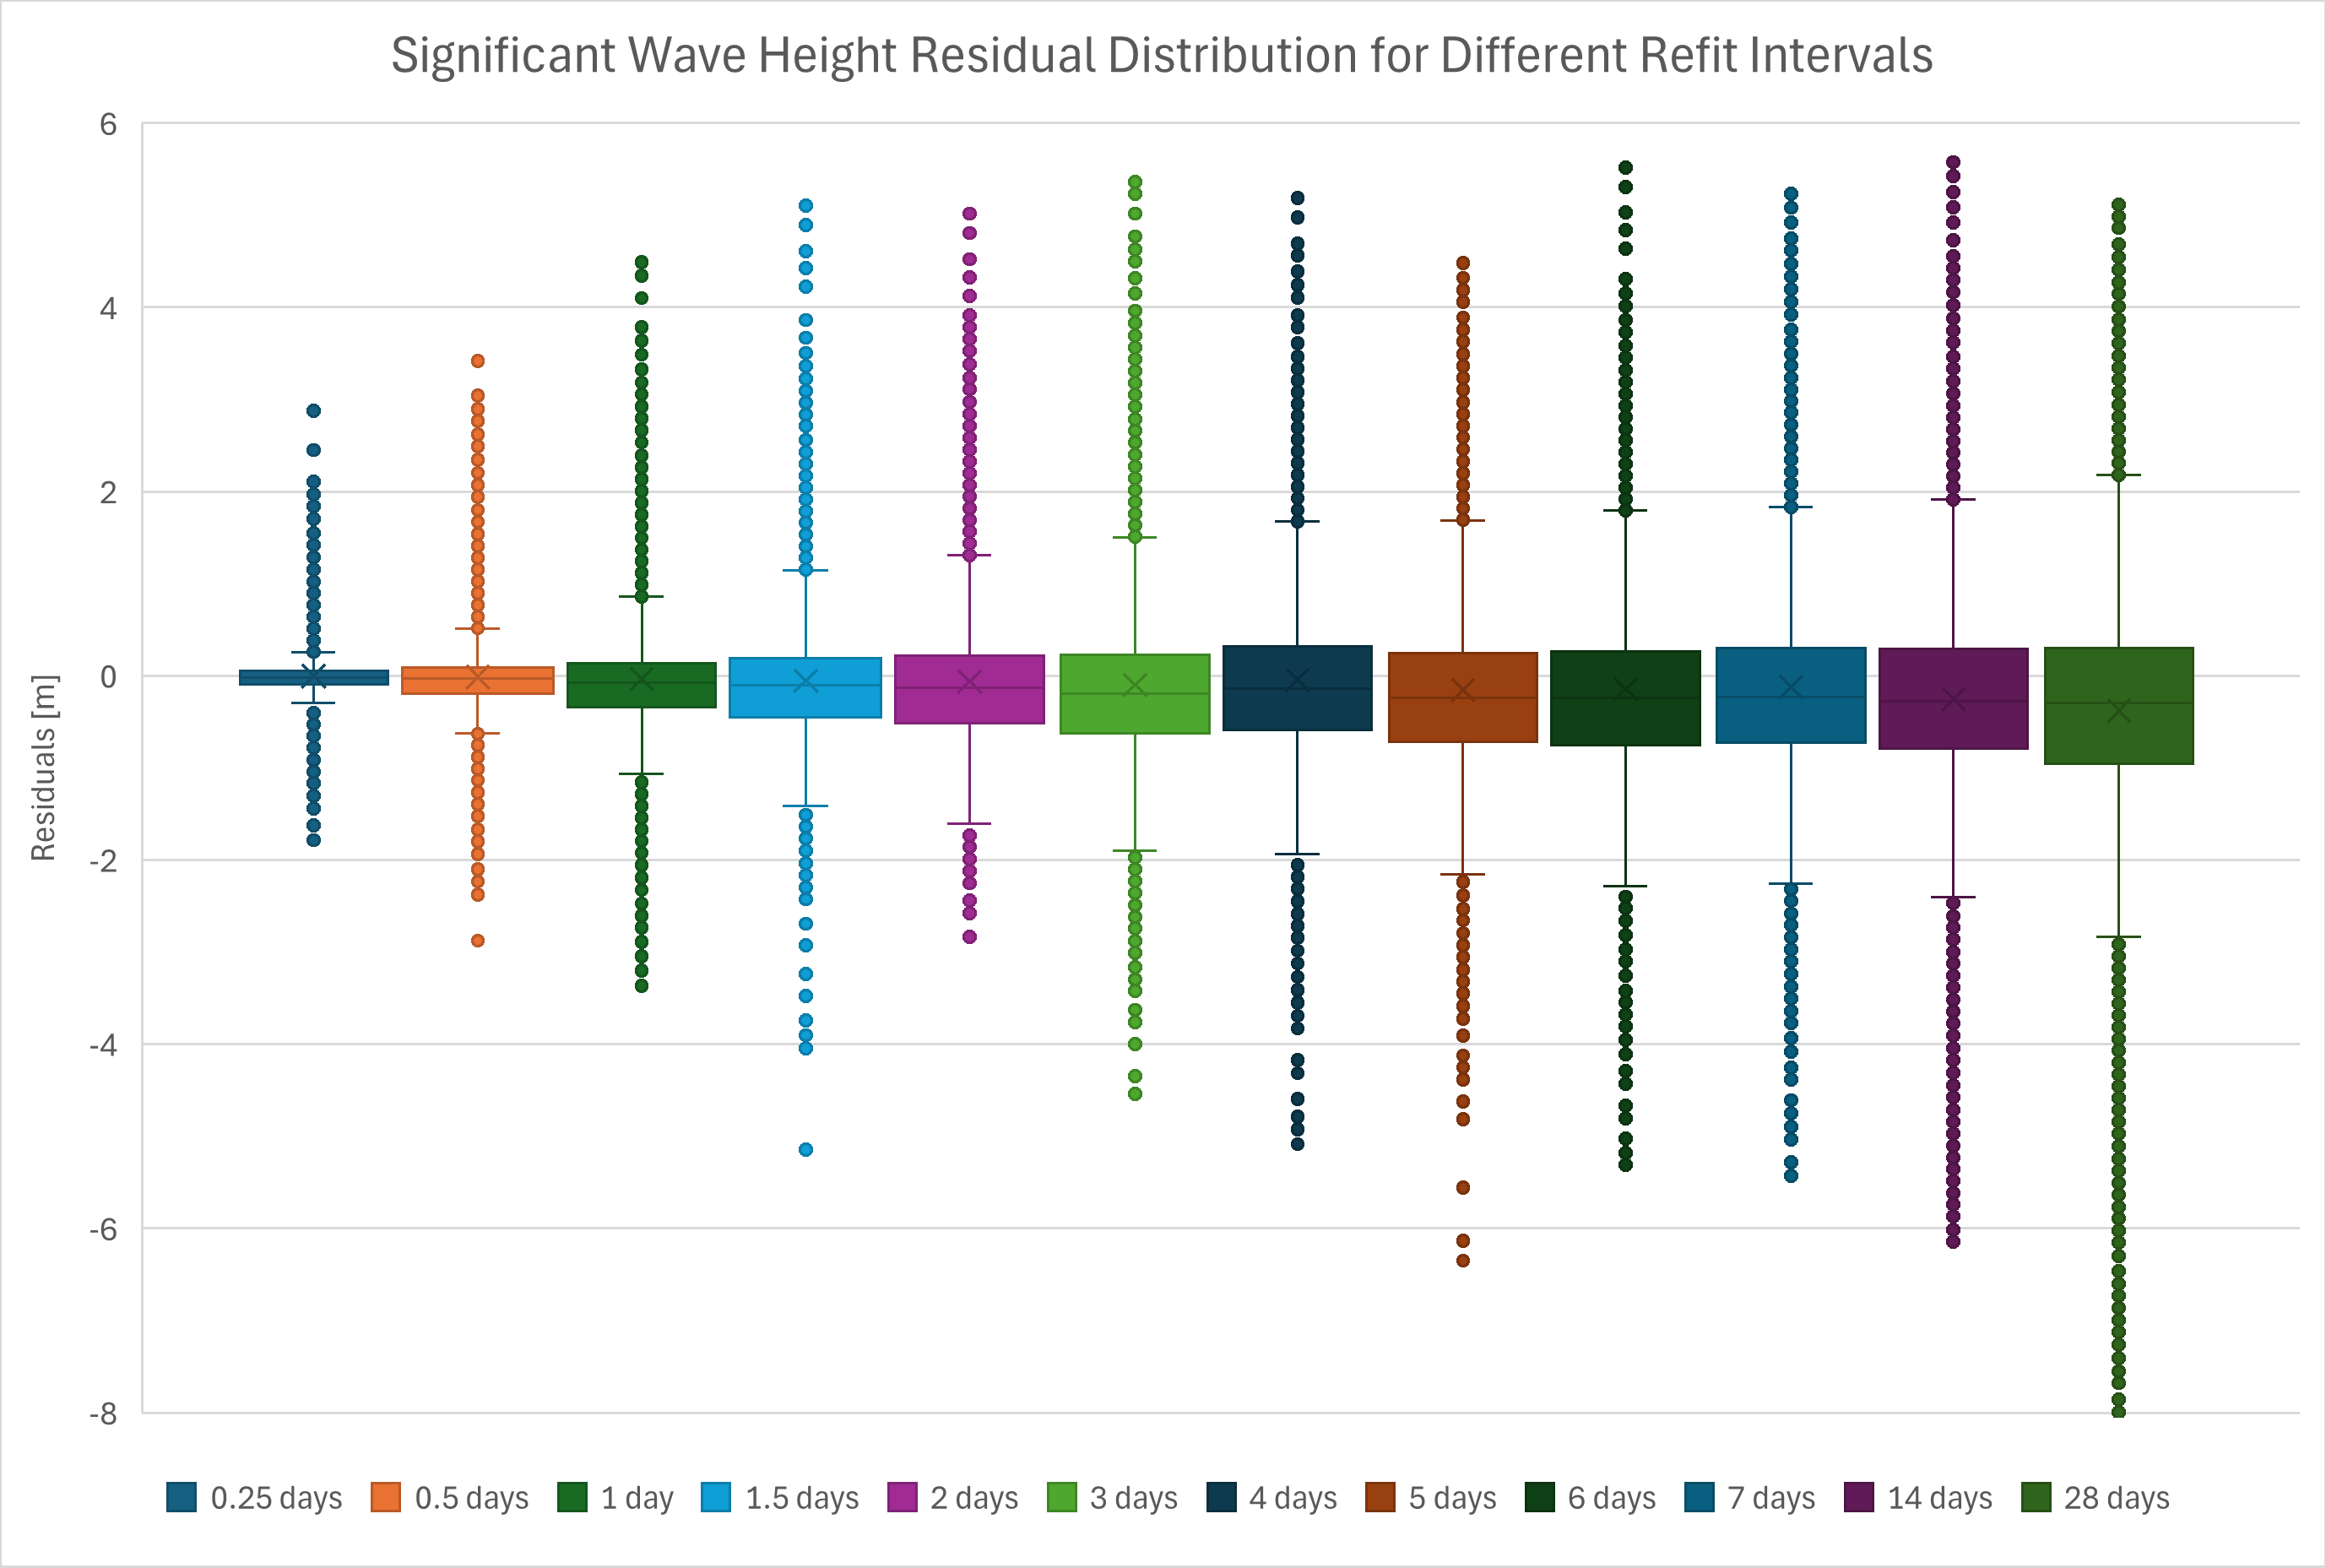
\includegraphics[width=\textwidth]{graphs/Box_refit_swht.png}
        \caption{Significant Wave Height}
        \label{fig:s_wht_refit_box}
    \end{subfigure}
    \hfill
    \begin{subfigure}[b]{0.49\textwidth}
        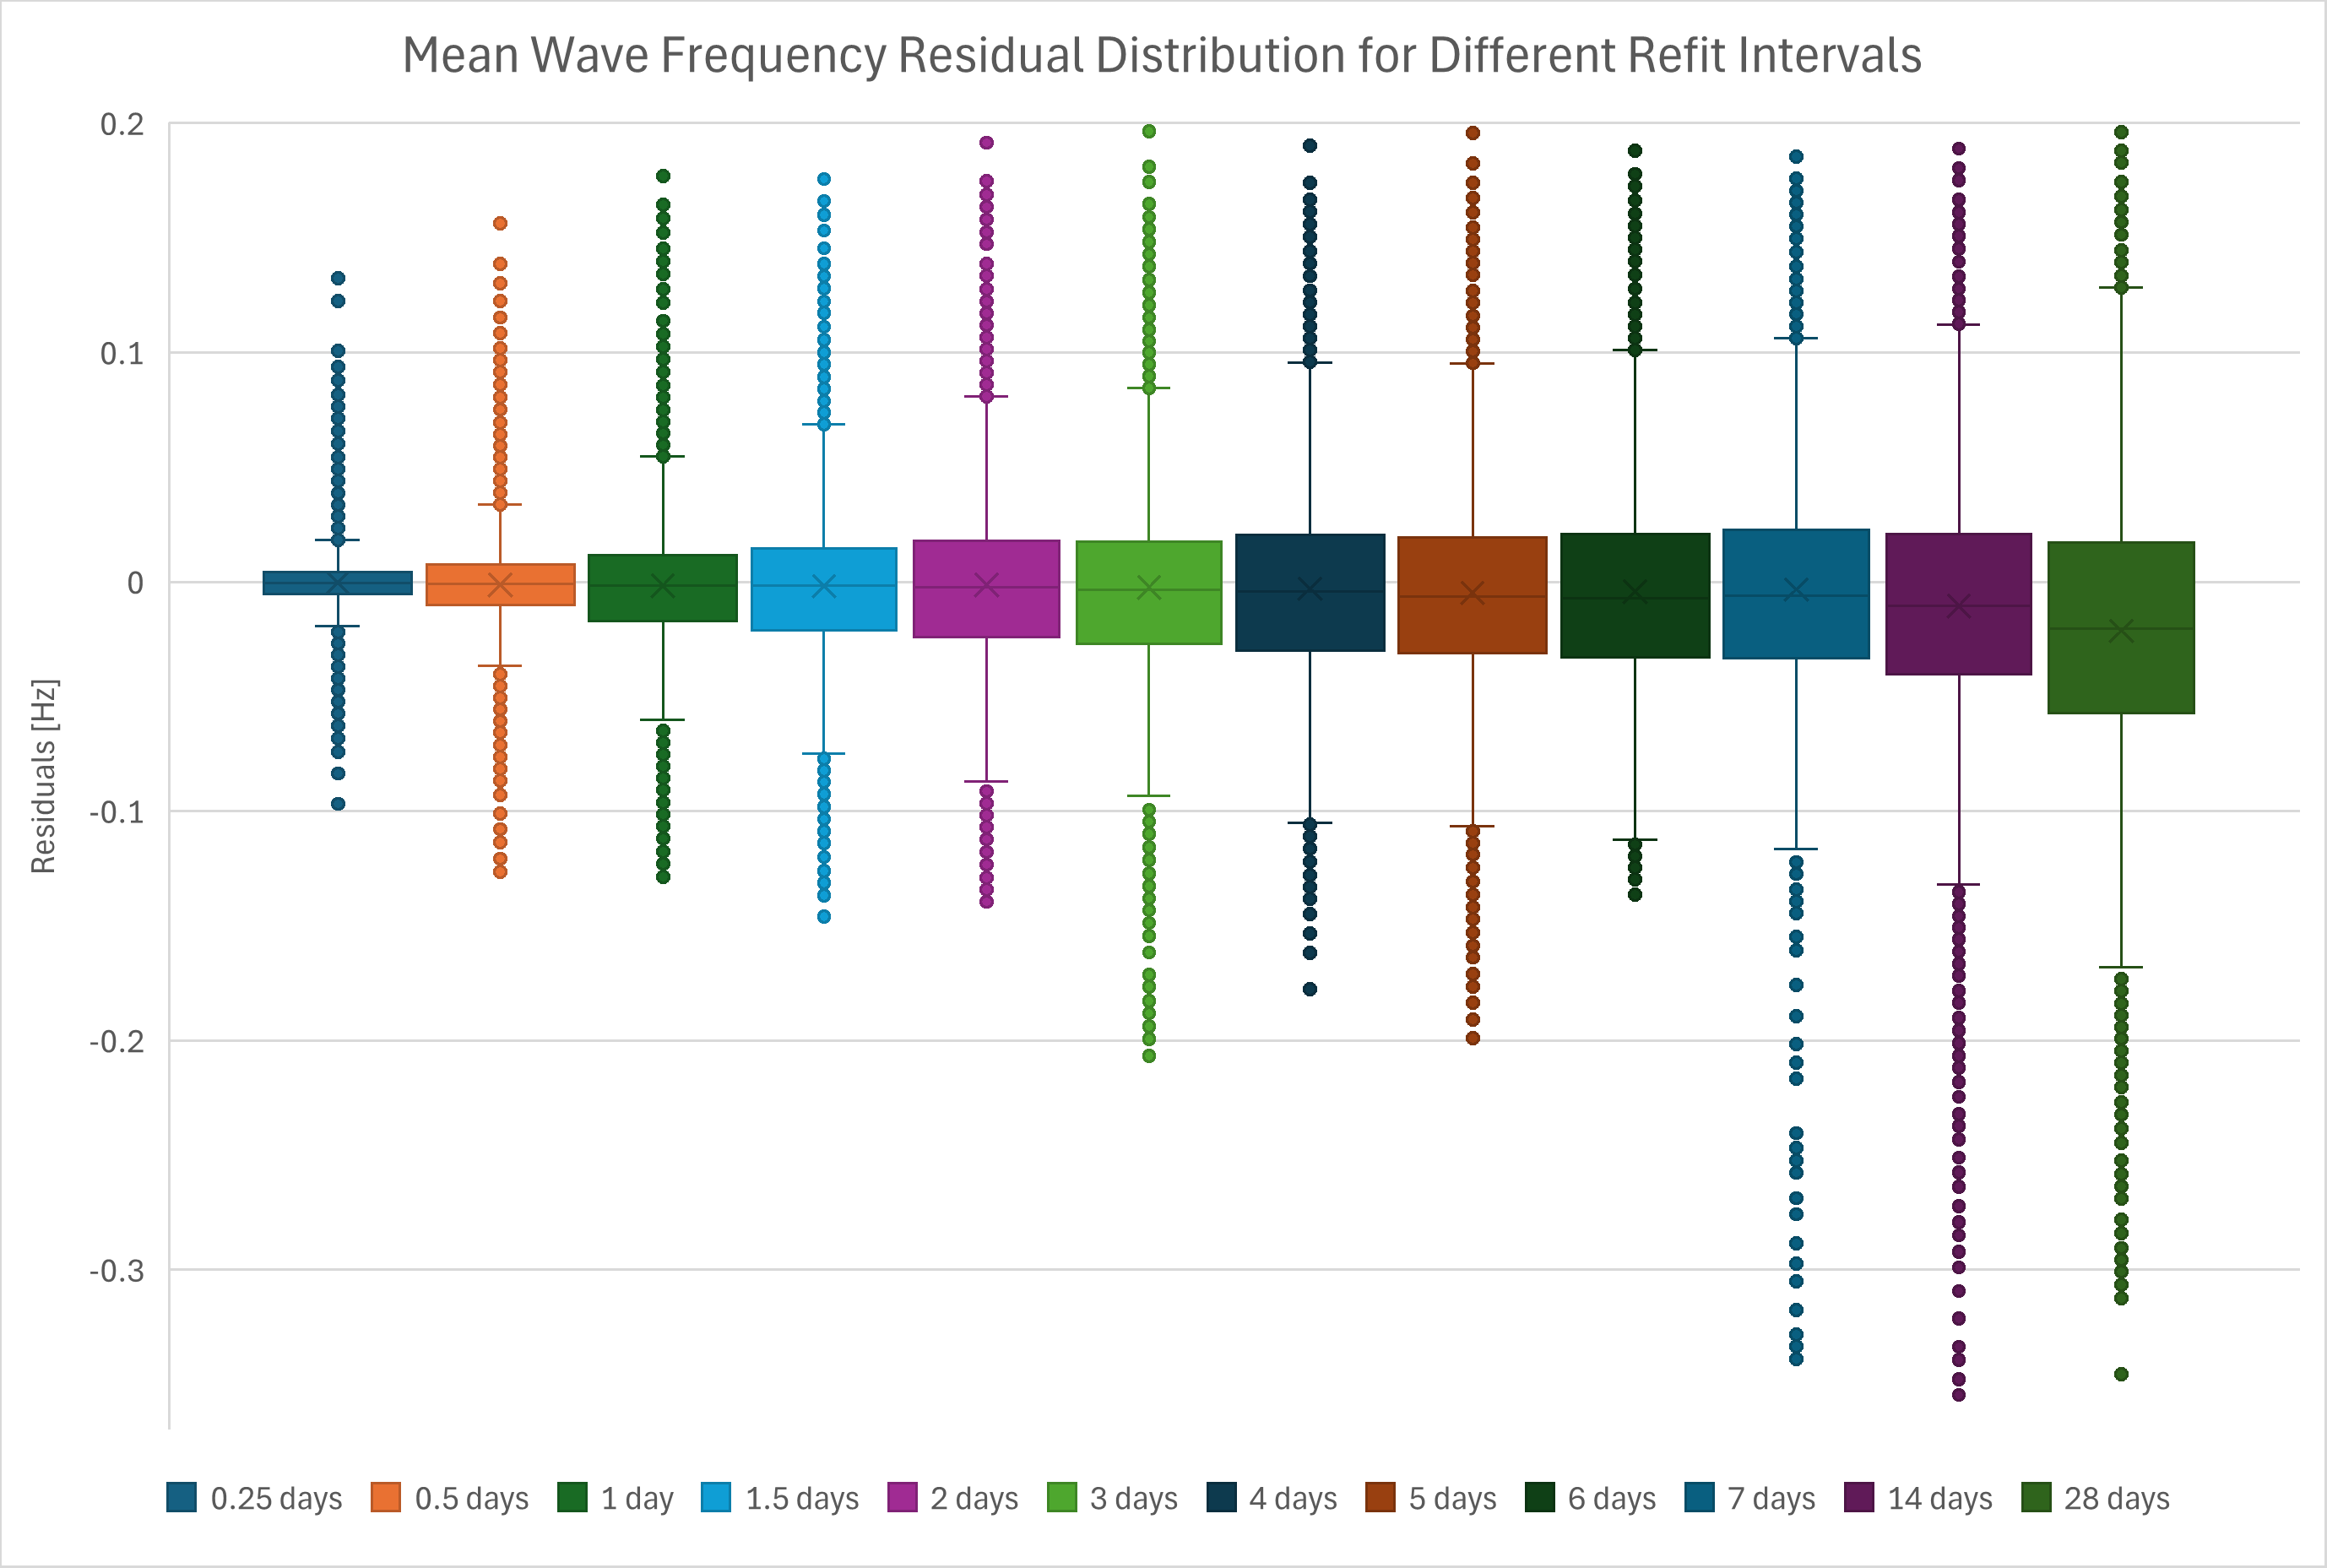
\includegraphics[width=\textwidth]{graphs/Box_refit_meanfr.png}
        \caption{Mean Wave Frequency}
        \label{fig:mean_fr_refit_box}
    \end{subfigure}
    \vskip\baselineskip
    \begin{subfigure}[b]{0.49\textwidth}
        \centering
        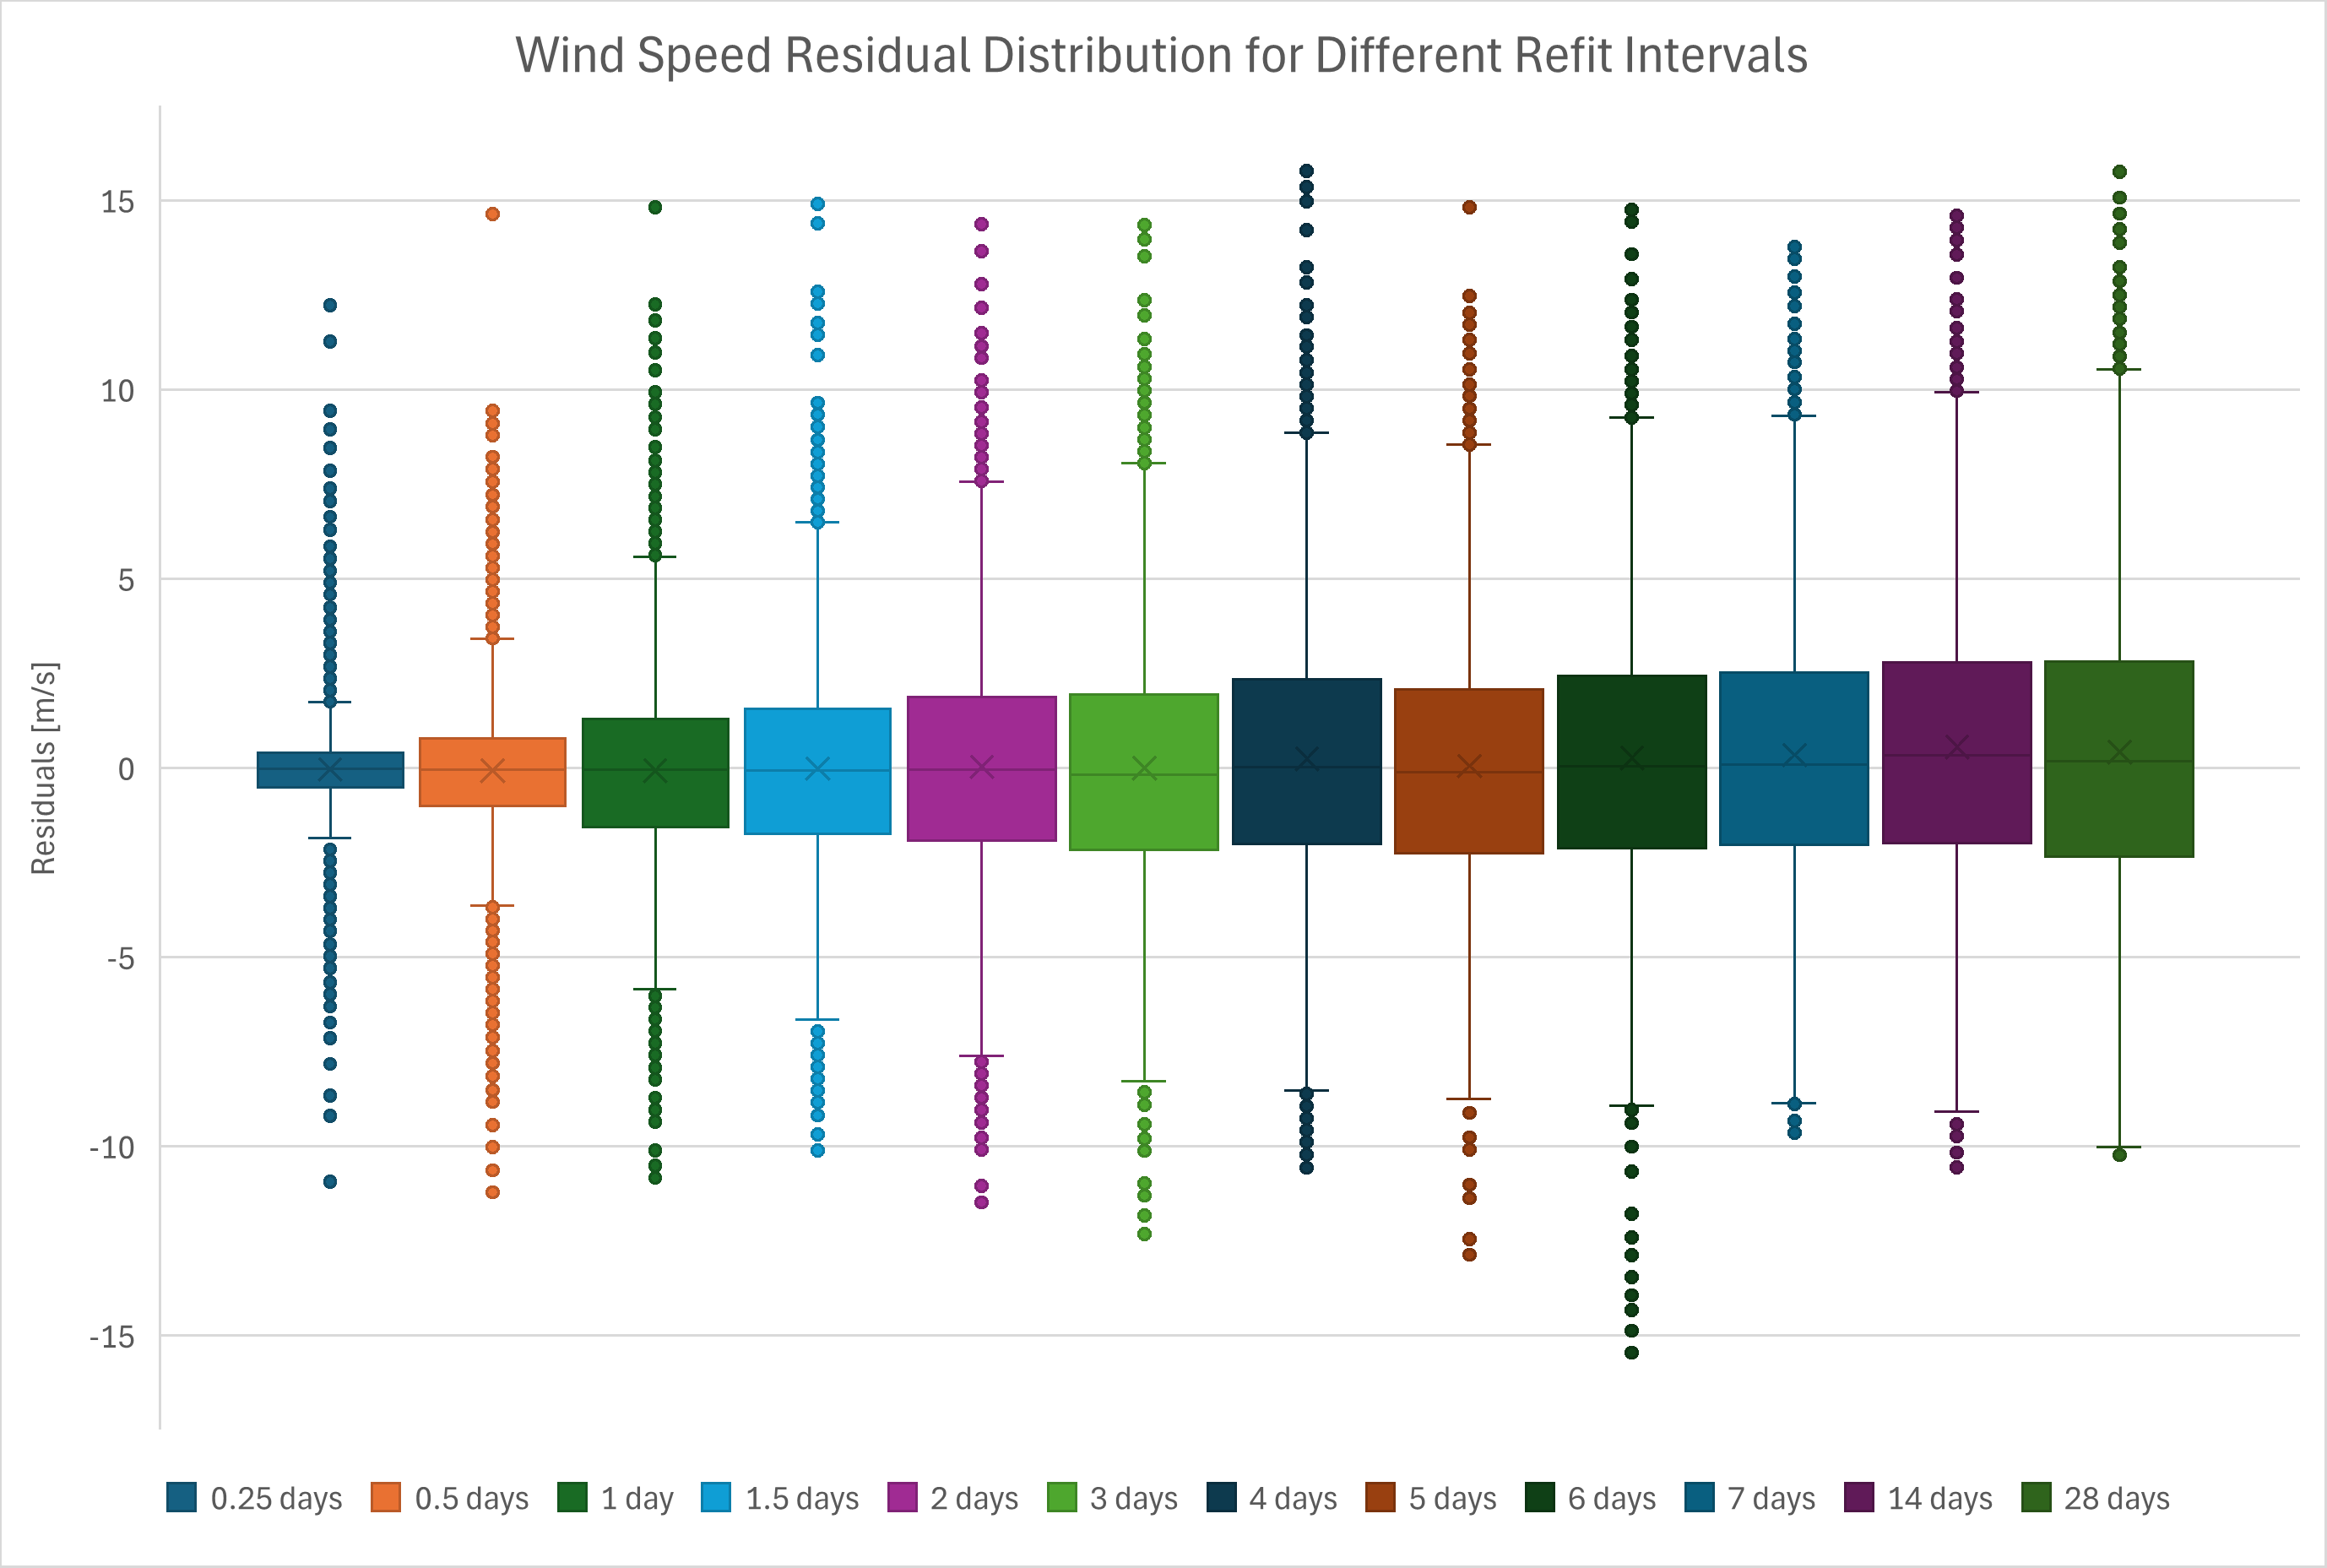
\includegraphics[width=\textwidth]{graphs/Box_refit_windspeed.png}
        \caption{Wind Speed}
        \label{fig:wind_speed_refit_box}
    \end{subfigure}
    \caption{Residual distribution of the Hybrid ARIMA–ANN model’s under varying refit intervals.}
    \label{fig:hybrid_refit_box}
\end{figure}

\newpage

\section{Implementation of Hybrid Model in Offshore Wind Turbine Installation}
\label{implementation_results}
From the operational limitations of the vessels for the mean wave frequency, from Table \ref{table:operational_limits}, it is seen that the mean wave frequency has a limit of 9 seconds and 7 seconds for respectively a Crane Barge and a Heavy Lift Vessel. Comparing this to the actual mean wave frequency in 2009, Figure \ref{fig:jack-up vessel usage}. It can be seen that in almost every case the mean wave frequency goes over the operational limit of both these vehicles. In practice, this means the installation will be done with a Jack-Up vessel.\\

\begin{figure}[ht!]
    \centering
    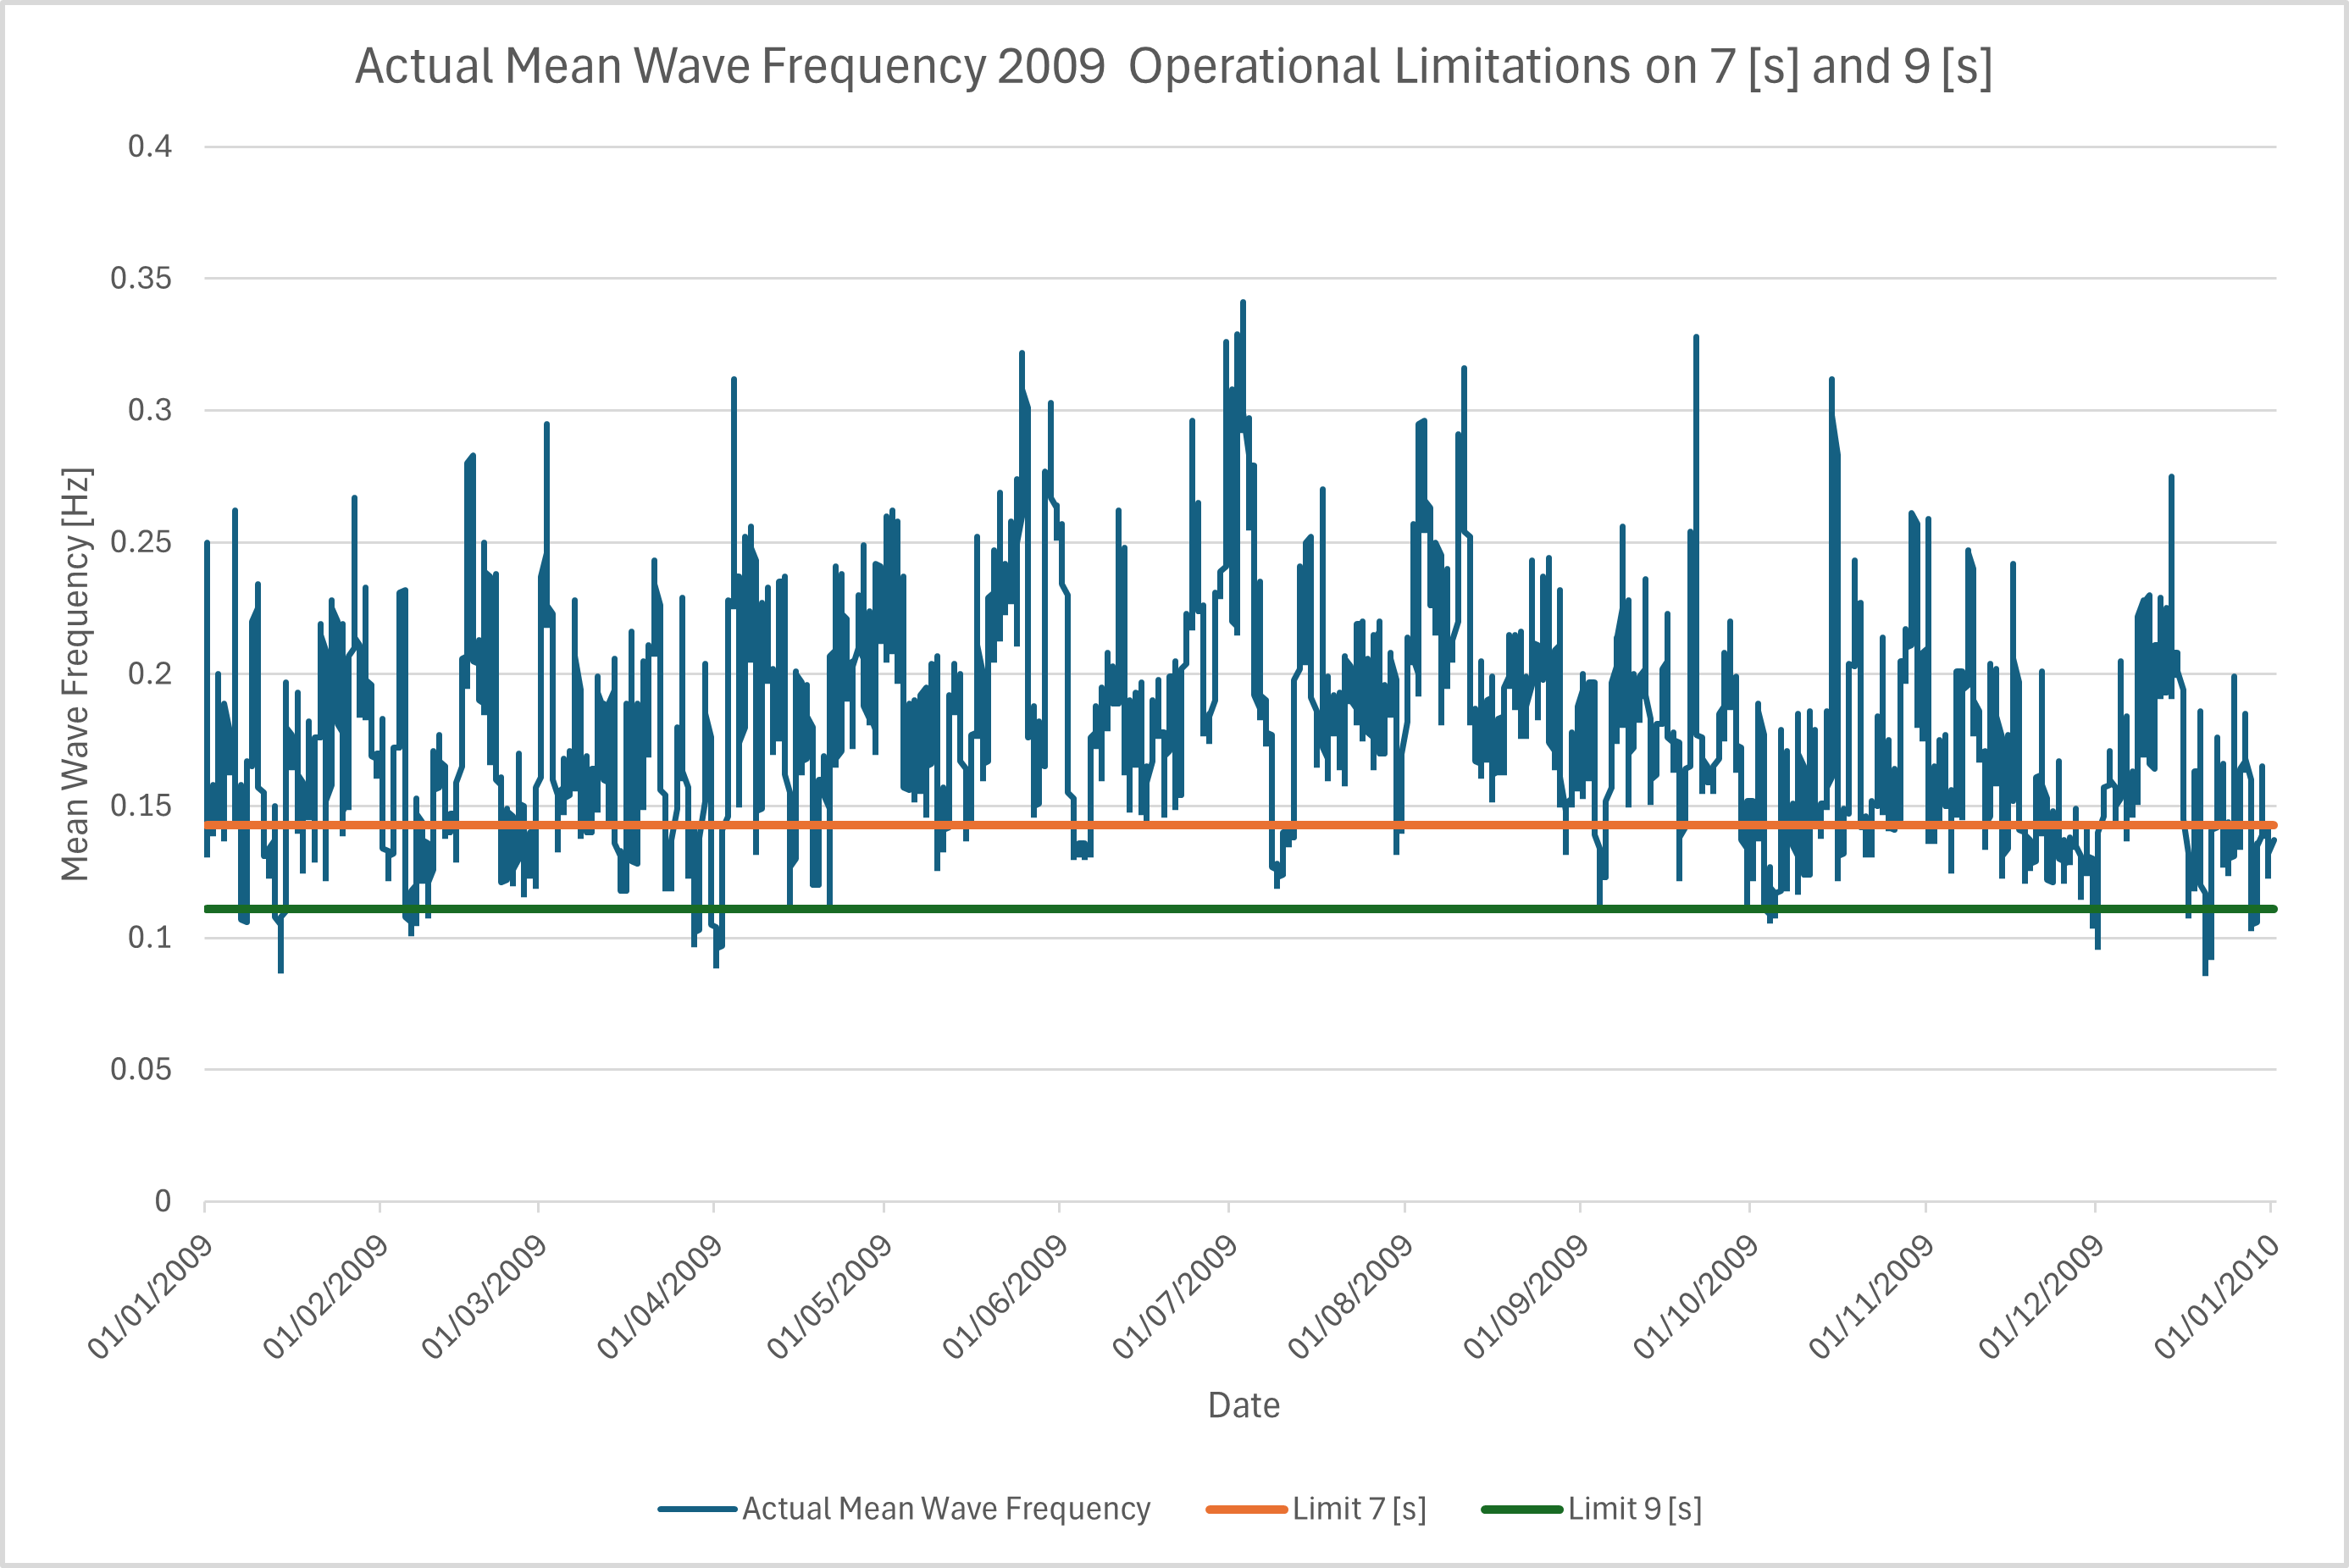
\includegraphics[width=0.6\linewidth]{graphs/Limitation on usage other ships then jack-up vessel.png}
    \caption{Operational limit for mean wave frequency of 7 and 9 [s]}
    \label{fig:jack-up vessel usage}
\end{figure}

\noindent The Operational Limitations of the Jack-Up Vessel from Table \ref{table:operational_limits} are re-shown below in Table \ref{table:operational_limits_jackup}. It follows that the Mean Wave Frequency does not influence the operational limits, so this will not be further investigated, the focus will be on the significant wave height and the wind speed. With their operational limitations, the actual outcomes of the Hybrid model are evaluated. A confusion matrix is constructed for both parameters and both limitations, with this the influence of different refit intervals is shown in Tables \ref{tab:swh_confusion_derived}, \ref{tab:wind_speed_8}, \ref{tab:wind_speed_10} and \ref{tab:wind_speed_16}.\\


\begin{table}[ht!]
    \centering
    \caption{Operational Limits for Key Weather Conditions During Installation Phases (Jack-Up Vessel)}
    \label{table:operational_limits_jackup}
    \begin{tabular}{|l|c|c|}
        \hline
        \textbf{Phase} & \textbf{Significant Wave Height} & \textbf{Wind Speed} \\
        \hline
        Monopile         & 2.5 & 16 \\
        \hline
        Transition Piece & 2.5 & 16 \\
        \hline
        Tower            & 2.5 & 10 \\
        \hline
        Nacelle          & 2.5 & 10 \\
        \hline
        Blade            & 2.5 & 8 \\
        \hline
    \end{tabular}
\end{table}

\noindent The confusion matrices below show the True Positive (TP), True Negatives (TN), False Positives (FP) and False Negatives (FN) for the model concerning the actual values. A TP occurs when the actual model and the forecast model both show a value above the limit, a TN when both are below. A FP when the forecast thinks the operational limit has been reached, but in practice this is not the case. FN is the most concerning, while the forecast thinks the operation could be done but the actual values are too high, which will lead to unsafe conditions. In the same manner FP would lead to stoppage of the installation, while unnecessary, and the costs associated with down-time. To further investigate these matrices, a False Positive Rate, a False Negative Rate and the Accuracy are calculated with the Formulas \ref{eq:fprate}, \ref{eqfnr} and \ref{eq:accuracy}.\\

\begin{equation}
\label{eq:fprate}
\text{FP Rate} = \frac{\text{False Positive}}{\text{False Positive} + \text{True Negative}}
\end{equation}

\begin{equation}
\label{eqfnr}
\text{FN Rate} = \frac{\text{False Negative}}{\text{False Negative} + \text{True Positive}}
\end{equation}

\begin{equation}
\label{eq:accuracy}
\text{Accuracy} = \frac{\text{True Positive} + \text{True Negative}}{\text{Total Observations}}
\end{equation}

\begin{table}[ht!]
    \centering
    \caption{Confusion Matrix and Derived Metrics for Significant Wave Height 2.5 m Operational Limit}
    \label{tab:swh_confusion_derived}
    \begin{tabular}{|l|c|c|c|c|c|c|c|c|}
        \hline
        \textbf{Refit Interval} & \textbf{TP} & \textbf{TN} & \textbf{FP} & \textbf{FN} && \textbf{FP Rate} & \textbf{FN Rate} & \textbf{Accuracy} \\
        \hline
        0.25 days & 2296 & 14661 & 232  & 331  && 1.56\%  & 12.60\% & 96.79\% \\
        0.5 days  & 2011 & 14462 & 431  & 616  && 2.89\%  & 23.45\% & 94.02\% \\
        1 day     & 1476 & 14135 & 758  & 1151 && 5.09\%  & 43.81\% & 89.10\% \\
        1.5 days  & 1139 & 14136 & 757  & 1488 && 5.08\%  & 56.64\% & 87.19\% \\
        2 days    & 882  & 14019 & 874  & 1745 && 5.87\%  & 66.43\% & 85.05\% \\
        3 days    & 570  & 13865 & 1028 & 2057 && 6.90\%  & 78.30\% & 82.39\% \\
        4 days    & 490  & 14074 & 819  & 2137 && 5.50\%  & 81.35\% & 83.13\% \\
        5 days    & 683  & 13677 & 1216 & 1944 && 8.16\%  & 74.00\% & 81.96\% \\
        6 days    & 429  & 13501 & 1392 & 2198 && 9.35\%  & 83.67\% & 79.51\% \\
        7 days    & 533  & 13841 & 1052 & 2094 && 7.06\%  & 79.71\% & 82.04\% \\
        14 days   & 701  & 13503 & 1390 & 1926 && 9.33\%  & 73.32\% & 81.07\% \\
        28 days   & 435  & 12360 & 2533 & 2192 && 17.01\% & 83.44\% & 73.03\% \\
        \hline
    \end{tabular}
\end{table}

\begin{table}[ht!]
    \centering
    \caption{Confusion Matrix and Derived Metrics for Wind Speed 8 m/s Operational Limit}
    \label{tab:wind_speed_8}
    \begin{tabular}{|l|c|c|c|c|c|c|c|c|}
        \hline
        \textbf{Refit Interval} & \textbf{TP} & \textbf{TN} & \textbf{FP} & \textbf{FN} && \textbf{FP Rate} & \textbf{FN Rate} & \textbf{Accuracy} \\
        \hline
        0.25 days & 6669 & 9374 & 686  & 791  && 6.82\%  & 10.60\% & 91.57\% \\
        0.5 days  & 5989 & 8923 & 1137 & 1471 && 11.30\% & 19.72\% & 85.11\% \\
        1 day     & 5137 & 8069 & 1991 & 2323 && 19.79\% & 31.14\% & 75.38\% \\
        1.5 days  & 4467 & 7636 & 2424 & 2993 && 24.10\% & 40.12\% & 69.08\% \\
        2 days    & 3866 & 7540 & 2520 & 3594 && 25.05\% & 48.18\% & 65.10\% \\
        3 days    & 3679 & 7224 & 2836 & 3781 && 28.19\% & 50.68\% & 62.23\% \\
        4 days    & 2739 & 7649 & 2411 & 4721 && 23.97\% & 63.28\% & 59.29\% \\
        5 days    & 3212 & 7224 & 2836 & 4248 && 28.19\% & 56.94\% & 59.57\% \\
        6 days    & 2730 & 7426 & 2634 & 4730 && 26.18\% & 63.40\% & 57.97\% \\
        7 days    & 2381 & 7625 & 2435 & 5079 && 24.20\% & 68.08\% & 57.11\% \\
        14 days   & 1977 & 7763 & 2297 & 5483 && 22.83\% & 73.50\% & 55.59\% \\
        28 days   & 1768 & 7837 & 2223 & 5692 && 22.10\% & 76.30\% & 54.82\% \\
        \hline
    \end{tabular}
\end{table}

\begin{table}[ht!]
    \centering
    \caption{Confusion Matrix and Derived Metrics for Wind Speed 10 m/s Operational Limit}
    \label{tab:wind_speed_10}
    \begin{tabular}{|l|c|c|c|c|c|c|c|c|}
        \hline
        \textbf{Refit Interval} & \textbf{TP} & \textbf{TN} & \textbf{FP} & \textbf{FN} && \textbf{FP Rate} & \textbf{FN Rate} & \textbf{Accuracy} \\
        \hline
        0.25 days & 3489 & 12959 & 417  & 655  && 3.12\%  & 15.81\% & 93.88\% \\
        0.5 days  & 2982 & 12719 & 657  & 1162 && 4.91\%  & 28.04\% & 89.62\% \\
        1 day     & 2098 & 12521 & 855  & 2046 && 6.39\%  & 49.37\% & 83.44\% \\
        1.5 days  & 1621 & 12601 & 775  & 2523 && 5.79\%  & 60.88\% & 81.18\% \\
        2 days    & 1194 & 12616 & 760  & 2950 && 5.68\%  & 71.19\% & 78.82\% \\
        3 days    & 924  & 12442 & 934  & 3220 && 6.98\%  & 77.70\% & 76.29\% \\
        4 days    & 557  & 12653 & 723  & 3587 && 5.41\%  & 86.56\% & 75.40\% \\
        5 days    & 848  & 12718 & 658  & 3296 && 4.92\%  & 79.54\% & 77.43\% \\
        6 days    & 642  & 12563 & 813  & 3502 && 6.08\%  & 84.51\% & 75.37\% \\
        7 days    & 552  & 12755 & 621  & 3592 && 4.64\%  & 86.68\% & 75.95\% \\
        14 days   & 369  & 12813 & 563  & 3775 && 4.21\%  & 91.10\% & 75.24\% \\
        28 days   & 482  & 12215 & 1161 & 3662 && 8.68\%  & 88.37\% & 72.47\% \\
        \hline
    \end{tabular}
\end{table}

\begin{table}[ht!]
    \centering
    \caption{Confusion Matrix and Derived Metrics for Wind Speed 16 m/s Operational Limit}
    \label{tab:wind_speed_16}
    \begin{tabular}{|l|c|c|c|c|c|c|c|c|}
        \hline
        \textbf{Refit Interval} & \textbf{TP} & \textbf{TN} & \textbf{FP} & \textbf{FN} && \textbf{FP Rate} & \textbf{FN Rate} & \textbf{Accuracy} \\
        \hline
        0.25 days & 127 & 17245 & 24  & 124 && 0.14\%  & 49.40\% & 99.16\% \\
        0.5 days  & 77  & 17231 & 38  & 174 && 0.22\%  & 69.32\% & 98.79\% \\
        1 day     & 46  & 17262 & 7   & 205 && 0.04\%  & 81.67\% & 98.79\% \\
        1.5 days  & 23  & 17262 & 7   & 228 && 0.04\%  & 90.84\% & 98.66\% \\
        2 days    & 28  & 17256 & 13  & 223 && 0.08\%  & 88.84\% & 98.65\% \\
        3 days    & 13  & 17269 & 0   & 238 && 0.00\%  & 94.82\% & 98.64\% \\
        4 days    & 24  & 17264 & 5   & 227 && 0.03\%  & 90.44\% & 98.68\% \\
        5 days    & 8   & 17266 & 3   & 243 && 0.02\%  & 96.81\% & 98.60\% \\
        6 days    & 14  & 17232 & 37  & 237 && 0.21\%  & 94.42\% & 98.44\% \\
        7 days    & 3   & 17269 & 0   & 248 && 0.00\%  & 98.80\% & 98.58\% \\
        14 days   & 0   & 17269 & 0   & 251 && 0.00\%  & 100.00\% & 98.57\% \\
        28 days   & 0   & 17269 & 0   & 251 && 0.00\%  & 100.00\% & 98.57\% \\
        \hline
    \end{tabular}
\end{table}

\noindent For the significant wave height in Table \ref{tab:swh_confusion_derived} it can be seen that the change between a 7-day refit interval and a 14-day refit interval does not influence the accuracy by a lot. Where there is a slight decrease in the accuracy, the large forecast window of 14 days would mean operations could be planned much longer in advance. In most cases, however, the significant wave height does not exceed the operational limit, as can be seen in the low amount of TP and FN values.\\

\noindent For Table \ref{tab:wind_speed_16} the operational limit is too high, which shows a model that is almost perfect in capturing it. For Tables \ref{tab:wind_speed_8} and \ref{tab:wind_speed_10} the relevance of accurate forecasting is evident. Especially for a wind speed of 8 [m/s], looking at the longer refit intervals in almost 50 \% of the cases the model fails to capture the limit correctly. With a high percentage of FN, but still a fairly low percentage for FP, the model. The same can be seen in Table \ref{tab:wind_speed_10} where more values are below the operational limit and so the model performs overall better.  

\chapter{Conclusion}
In this Chapter, the research questions and sub-questions are answered from the results. The report aims to improve weather forecasts for significant wave height, mean wave frequency, and wind speed for offshore wind turbine installations by comparing hybrid, probabilistic, and deep learning models, and what is the impact of varying refit intervals on forecast performance?.

\subsection*{Sub-Questions}
\noindent \textbf{What are the strengths and limitations of hybrid, probabilistic, and deep learning models for forecasting key weather conditions in offshore wind turbine installation?}

\noindent The Hybrid ARIMA-ANN model captured the wave height fluctuations and peaks well, but it required careful tuning during the construction of the model. The Bayesian Neural Network with Monte Carlo Dropout can show uncertainty estimations, which could be beneficial for risk assessment. But, it does show a higher variance and higher values for the evaluation metrics. The strengths of the LSTM model will be in the shorter forecasting, when the fluctuations are not relevant. Another shortcoming of this model is the large data set necessary to make a well-established trained model. \\

\noindent \textbf{How do the BNN with Monte Carlo Dropout, LSTM, and Hybrid ARIMA–ANN compare in forecasting significant wave height, wave frequency, and wind speed using a 5-day refit interval?}

\noindent At the 5-day refit interval, it showed the Hybrid model had some values for the coefficient of determination ($R^2$) that indicated that it is performing worse than a naive baseline. Although, overall the forecast was able to capture the fluctuations and the other evaluation metrics are kept to a minimum. BNN with MC dropout showed wider residual spread, which is not beneficial in accurate forecasting, and so causes worse evaluation metrics compared to the other models. The LSTM model, although performing similarly as the Hybrid model based on the evaluation metrics, it is not capturing any fluctuations between the refit intervals.\\

\noindent \textbf{How does the Hybrid ARIMA–ANN model’s performance change with varying refit intervals, when the model is retrained with the actual past data (6 hours, 12 hours, 1 day, 2 days, 3 days, 4 days, 5 days, 6 days, 7 days, 1 week, 2 weeks and 4 weeks)?}

\noindent Frequent refitting (\leq 1-day) improved the forecasts, almost halving the errors in the evaluation metrics. It is important to note that with these shorter refit intervals comes the increase in computational time. There needs to be a weigh-off on how accurate the model has to be and how many days ahead the forecast needs to be.

\newpage 

\noindent \textbf{What are the implications of these forecasting models and intervals for scheduling and risk management in offshore wind farm installation?}

\noindent The longer refit intervals increase the chance of missed dangerous conditions (FN), which will give higher safety risks for the installation phase. Shorter refit intervals lead to a higher accuracy and so lower values for false negatives and false positives. There needs to be a weighing of how far the forecast should be ahead of time and what amount of risks an operator is willing to take. For now, a refit interval of 1 day would be a good weight off between these values, where the accuracy is still fairly high and the risks associated with this accuracy are low. 

\subsection*{Research Question}  
How can weather forecasts for significant wave height, mean wave frequency, and wind speed be improved for offshore wind turbine installations by comparing hybrid, probabilistic, and deep learning models, and what is the impact of varying refit intervals on forecast performance?\\

\noindent By comparing the three models, it can be concluded that the Hybrid ARIMA-ANN model outperformed the other two models. Though the LSTM performed similarly by RMSE/MAE, it did not respond as well to short-term spikes within the 5-day interval. This indicates it may need a shorter refit interval or a larger dataset to adapt to sudden changes. The Bayesian Neural Network with Monte Carlo dropout, although high computational time, gives a higher variance in the model. The Hybrid model captures the fluctuations in the data and, in the meantime, also ensures the errors are kept to a minimum. For a \leq 1-day refit intervals, the model showed consistent accurate forecasts of Significant Wave Height and Wind Speed. This will reduce the likelihood of dangerous situations, and overall it will lead to a smoother operation.
\chapter{Discussion}

\section{Three model comparison}
The main goal of this research was to increase the accuracy in the forecasting of Significant Wave Height, Mean Wave Frequency and Wind Speed. This is to ensure the operational windows for the installation of offshore wind-turbines can be used optimally. Three different forecast models were designed with each having their strengths and limitations, shown in Table \ref{tab:model_comparison}. 

\begin{table}[ht!]
\centering
\begin{tabular}{|p{4cm}|p{6cm}|p{6cm}|}
\hline
\textbf{Model} & \textbf{Strengths} & \textbf{Limitations} \\
\hline
Hybrid ARIMA–ANN & 
Balances linear and non-linear patterns by combining a linear approximation (ARIMA) with a neural network’s capability to capture the non-linear data. &
Relies on consistently strong ARIMA residual modelling – unexpected real-world outliers may affect the ANN’s ability to effectively capture non-linear outliers. \\
\hline
Bayesian Neural Network (BNN) with Monte Carlo Dropout (MCD) & 
Provides predictive distributions rather than point estimates, enabling detailed risk assessment for scheduling and operations. &
Tends to have higher computational time and careful calibration of dropout rates to avoid over- or under-estimating uncertainty. \\
\hline
Long Short-Term Memory (LSTM) & 
Can be used on shorter refit intervals where the fluctuations in the data are lower, there it will be highly accurate where it captures most of the values within a certain range. &
There needs to be more than enough training data to ensure the model captures all outliers, if not available the model will not perform well. The exponential approximation might not always suit the data. \\
\hline
\end{tabular}
\caption{Comparison of Model Strengths and Limitations}
\label{tab:model_comparison}
\end{table}

\noindent When these models are applied to the data, all three models showed new insights and advantages in the forecasting of significant wave height, mean wave frequency and wind speed. The level of improvement although, was different between the models, where the Hybrid and the BNN with MC dropout were able to capture the fluctuations within the data. The LSTM model had some shortcomings, this can be caused by not enough available training data, or the hyperparameter needs to be further tuned. 

\section{Refit Intervals}
The Hybrid ARIMA-ANN model showed the most promising results with a 5-day refit interval, where the residuals were within a respectable range, Figure \ref{fig:combined_box}, and the evaluation metrics, Table \ref{tab:performance_comparison}, showed the errors are small. With the short refit intervals \leq 1-day, the model is highly adaptive, and short-term forecasting becomes very accurate. The computational time does increase while the model needs to be retrained every time a new refit interval occurs. With longer intervals \geq 1-day this time is dropped significantly, but at a cost of a less accurate model. \\

\noindent In the implementation of the forecast model, there needs to be a weighing off between the accuracy, the computational time and how far into the future the forecast should reach. This will be specific for each site and on each operation, depending on different factors like vessel rental costs, local weather conditions, and financial tolerances.  

\section{Implications for Offshore Wind Turbine Installation}
In real-life installations, the implication of the forecasts will need to reduce the waiting time when a vessel cannot be used. From Table \ref{table:operational_limits}, the different vessels are all suitable in different scenarios. Where, due to the investigated site, only a jack-up vessel is an option. Where other sites might have lower values, for the significant wave height, the mean wave frequency and the wind speed, the use of other vessels would be optional. This will lead to more availability during the installation, which could lead to a smoother and more efficient installation. 

\section{Limitations of the Present Research}
While the Hybrid model does show some accurate forecasts, it is important to note some of the limitations during this research:
\begin{itemize}
    \item \textbf{Geographical scope}: As discussed earlier, only one site was analysed, different sites might have different forecast behaviour. 
    \item \textbf{Data complexity} Where only Significant Wave Height, Mean Wave Frequency and Wind Speed were used, other parameters could further refine the forecast.
    \item \textbf{Computational Constraints} Due to long computational times, the models are somewhat scoped, which leads to a less accurate model overall.
\end{itemize}

Although the results show the importance of matching the forecasts with the operational installation. Advanced models can be used to make the forecasts, but the implementation needs to be carefully assessed in real-world cases.
\chapter{Recommendations}
During the construction of the models, there are some parts that fall beyond this research. For future researches the following recommendations are made. Firstly, the model implementation in operational settings in Section \ref{model implementation in operational settings}. Secondly, the optimizing of the refit intervals in Section \ref{optimizing refit intervals}. For future researches conducted on the subject, some directions are mad in Section \ref{future research directions}. 

\section{Model Implementation in Operational Settings}
\label{model implementation in operational settings}
Implementing the currently designed advanced forecasting techniques in real-world situations should be done based on what needs to be forecasted. The Hybrid model is most applicable in routine scheduling, by generating 1-day forecasts. The model is relatively easy to implement and the improved accuracy, with the use of basic methods help to reduce operational uncertainty. The Bayesian Neural Network with Monte Carlo dropout is most applicable for high-risk operations, where the model can generate a predictive distribution of the forecasts. This can guide the operators to make a decision on when the operation could be executed. LSTM models can be used in regions that suffer from rapid weather changes, although the computational resources to refit often limits this forecast model.

\section{Optimizing Refit Intervals}
\label{optimizing refit intervals}
To be able to optimize the refit intervals it is important to know how the weather behaves of a certain time frame. Tailored intervals could give a solution, by using an adaptive refit interval which can be switched to a shorter interval during storms, the forecasts could be made more accurate. Keeping in mind this might not be beneficial for sites where a longer forecast is necessary.\\

\section{Future Research Directions}
\label{future research directions}
Where right now the research was focused on one site, a \textbf{Multi-Site Validation} would extend the analyses of these models. Different met-ocean conditions on different sites, with different depths could generalize the model performance and identify site-specific best practices. \textbf{Expanding the Parameter Set}, the models are now only based on their own trained values, exogenous parameters like wind direction, tides or swells could be included. This will probably lead to a model with higher accuracy, but at a cost of again a longer computational time. When models are implemented pm the sites \textbf{Real-Time Continuous Learning} could be applied. Finding a way to continuously retrain the model with real-time data, where the models will update/refit every time a new measurement is done. This is especially useful in short-term forecasting. \textbf{A Hybrid Probabilistic model} investigate if a combination of the Hybrid ARIMA-ANN model with the Bayesian Neural Network is possible. In this case the model would be able to not only make a accurate forecast, but also the distribution of the forecasts could be used in risk assessments. 
%% Use letters for the chapter numbers of the appendices.
\cleardoublepage % Ensure the appendices start on a new page
\renewcommand{\chaptername}{Appendix}
\appendix
\setcounter{chapter}{0} % Reset chapter counter for appendices

%\chapter{Python Code Operational Limits} % Add Appendix A
%\label{append:operational limit}
\begin{minted}[frame=lines, breaklines, fontsize=\small]{python}
import pandas as pd
import matplotlib.pyplot as plt

file_path = '/Users/maxcrebolder/Documents/Site15_29m.xlsx'

xls = pd.ExcelFile(file_path)
dfs_s_wht = []
dfs_mean_fr = []
dfs_wind_speed = []

for sheet in xls.sheet_names:
    df = pd.read_excel(xls, sheet_name=sheet)
    dfs_s_wht.append(df[['s_wht']])       
    dfs_mean_fr.append(1 / df[['mean_fr']]) 
    dfs_wind_speed.append(df[['wind_speed']])  

wave_data_s_wht = pd.concat(dfs_s_wht, axis=1)
wave_data_mean_fr = pd.concat(dfs_mean_fr, axis=1)
wave_data_wind_speed = pd.concat(dfs_wind_speed, axis=1)

wave_data_s_wht['Average_s_wht'] = wave_data_s_wht.mean(axis=1)
wave_data_mean_fr['Average_mean_fr'] = wave_data_mean_fr.mean(axis=1)
wave_data_wind_speed['Average_wind_speed'] = wave_data_wind_speed.mean(axis=1)

plt.figure(figsize=(12, 8))
plt.plot(wave_data_s_wht['Average_s_wht'], label='Average s_wht', color='blue')
plt.axhline(y=2.5, color='red', linestyle='--', label='Operational limit (y=2.5)')
plt.title("Average Significant Wave Height Over Time Site 1")
plt.xlabel("Hour")
plt.ylabel("Average Significant Wave Height (s_wht)")
plt.legend(loc='upper right', fontsize=20) 
plt.grid(True)
plt.tight_layout()
plt.show()

plt.figure(figsize=(12, 8))
plt.plot(wave_data_mean_fr['Average_mean_fr'], label='Average 1/mean_fr', color='blue')
plt.axhline(y=9, color='red', linestyle='--', label='Operational limit (y=9)')
plt.axhline(y=7, color='orange', linestyle='--', label='Operational limit (y=7)')
plt.title("Average Mean frequency Over Time Site 1")
plt.xlabel("Hour")
plt.ylabel("Average 1/Mean Frequency (1/mean_fr)")
plt.legend(loc='upper right', fontsize=20)  
plt.grid(True)
plt.tight_layout()
plt.show()

plt.figure(figsize=(12, 8))
plt.plot(wave_data_wind_speed['Average_wind_speed'], label='Average wind_speed', color='blue')
plt.axhline(y=16, color='red', linestyle='--', label='Operational limit (y=16)')
plt.axhline(y=10, color='orange', linestyle='--', label='Operational limit (y=10)')
plt.axhline(y=8, color='yellow', linestyle='--', label='Operational limit (y=8)')
plt.title("Average Wind Speed Over Time Site 1")
plt.xlabel("Hour")
plt.ylabel("Average Wind Speed")
plt.legend(loc='upper right', fontsize=20)  
plt.grid(True)
plt.tight_layout()
plt.show()
\end{minted}

%\chapter{Hybrid script: ARIMA-ANN Model}
%\label{append:hybrid_script}
\begin{minted}[frame=lines, breaklines, fontsize=\small]{matlab}
clc; close all;

%% Configuration
file_path       = "C:\Users\maxcr\OneDrive\Documenten\Research assignment\Data\Site15_29m.xlsx";
parameters      = {'s_wht','mean_fr','wind_speed'};
years           = 2001:2010;
training_years  = 2001:2008;
testing_years   = 2009:2010;

hours_per_day   = 24;
hours_per_refit = 5 * hours_per_day;  
refitFrequency  = 1; 
rollingWindowHours = 150 * 24;  

modelConfigs = struct;
modelConfigs.s_wht.arimaOrder      = [2 0 3];
modelConfigs.s_wht.windowSize      = 149;
modelConfigs.s_wht.hiddenLayerSize = 5;
modelConfigs.s_wht.trainFcn        = 'trainlm';
modelConfigs.s_wht.maxEpochs       = 15;
modelConfigs.s_wht.goal            = 1e-6;

modelConfigs.mean_fr.arimaOrder      = [2 0 3];
modelConfigs.mean_fr.windowSize      = 149;
modelConfigs.mean_fr.hiddenLayerSize = 15;
modelConfigs.mean_fr.trainFcn        = 'trainlm';
modelConfigs.mean_fr.maxEpochs       = 30;
modelConfigs.mean_fr.goal            = 1e-6;

modelConfigs.wind_speed.arimaOrder      = [2 0 3];
modelConfigs.wind_speed.windowSize      = 48;
modelConfigs.wind_speed.hiddenLayerSize = 15;
modelConfigs.wind_speed.trainFcn        = 'trainlm';
modelConfigs.wind_speed.maxEpochs       = 25;
modelConfigs.wind_speed.goal            = 1e-6;

%% Load and Preprocess Data
disp('Loading and preprocessing data...');
allData = struct();
for iYear = 1:length(years)
    try
        tbl = readtable(file_path, 'Sheet', num2str(years(iYear)));
    catch ME
        error('Error reading sheet %d (%d): %s', iYear, years(iYear), ME.message);
    end
    for p = 1:length(parameters)
        pName = parameters{p};
        if ismember(pName, tbl.Properties.VariableNames)
            tempData = tbl.(pName);
            tempData = fillmissing(tempData, 'linear');
        else
            tempData = nan(height(tbl),1);
        end
        allData(iYear).(pName) = tempData;
    end
end

trainData   = struct();
testData    = struct();
normParams  = struct();

for p = 1:length(parameters)
    pName = parameters{p};
    trainVals = [];
    for y = training_years
        idx = find(years == y);
        trainVals = [trainVals; allData(idx).(pName)];
    end
    testVals = [];
    for y = testing_years
        idx = find(years == y);
        testVals = [testVals; allData(idx).(pName)];
    end

    [trainNorm, ps] = mapminmax(trainVals', 0, 1);
    trainNorm = trainNorm';
    testNorm  = mapminmax('apply', testVals', ps);
    testNorm  = testNorm';

    trainData.(pName)   = trainNorm;
    testData.(pName)    = testNorm;
    normParams.(pName)  = ps;
end

%% Initial ARIMA + ANN Training
disp('Initial ARIMA + ANN training...');
tempModels = cell(1, length(parameters));
options = optimoptions('fmincon', 'Display','off', 'MaxIterations',100, 'MaxFunctionEvaluations',200);

parfor p = 1:length(parameters)
    pName = parameters{p};
    arima_fit = [];
    try
        arimaOrder = modelConfigs.(pName).arimaOrder;
        if arimaOrder(1) > 0, ARLags = 1:arimaOrder(1); else, ARLags = []; end
        if arimaOrder(3) > 0, MALags = 1:arimaOrder(3); else, MALags = []; end
        arima_spec = arima('Constant', NaN, 'ARLags', ARLags, ...
                           'D', arimaOrder(2), 'MALags', MALags);
        arima_fit = estimate(arima_spec, trainData.(pName), 'Display','off','Options', options);
    catch ME
        if strcmp(pName, 's_wht')
            fallbackOrder = [2 0 1];
            try
                if fallbackOrder(1)>0, ARLags = 1:fallbackOrder(1); else, ARLags=[]; end
                if fallbackOrder(3)>0, MALags = 1:fallbackOrder(3); else, MALags=[]; end
                fallback_spec = arima('Constant', NaN, 'ARLags',ARLags, ...
                                      'D',fallbackOrder(2), 'MALags',MALags);
                arima_fit = estimate(fallback_spec, trainData.(pName), 'Display','off','Options', options);
            catch
                arima_fit = [];
            end
        else
            arima_fit = [];
        end
    end

    windowSize     = modelConfigs.(pName).windowSize;
    hiddenLayerSz  = modelConfigs.(pName).hiddenLayerSize;
    trainFcn       = modelConfigs.(pName).trainFcn;
    maxEpochs      = modelConfigs.(pName).maxEpochs;
    goalVal        = modelConfigs.(pName).goal;
    [Xann, Yann]   = createANNData(trainData.(pName), windowSize);

    net = feedforwardnet(hiddenLayerSz, trainFcn);
    net.trainParam.showWindow      = false;
    net.trainParam.showCommandLine = false;
    net.trainParam.epochs = maxEpochs;
    net.trainParam.goal   = goalVal;
    net = train(net, Xann', Yann');

    tempModels{p} = struct('arima', arima_fit, ...
                           'ann', net, ...
                           'window', windowSize, ...
                           'trainingData', trainData.(pName), ...
                           'cumulativeErrors', struct('ARIMA',1, 'ANN',1));
end

models = cell2struct(tempModels, parameters, 2);

%% Rolling Forecast & Re-Fit
disp('Starting rolling forecast/refit...');
forecasts = struct(); 
residuals = struct(); 
metrics   = struct();

for p = 1:length(parameters)
    pName = parameters{p};
    nTest = length(testData.(pName));
    forecasts.(pName) = nan(nTest,1);
    residuals.(pName) = nan(nTest,1);
    metrics.(pName).MSE  = [];
    metrics.(pName).MAE  = [];
    metrics.(pName).RMSE = [];
    metrics.(pName).R2   = [];
end

numTestSamples = length(testData.(parameters{1}));
numBlocks = ceil(numTestSamples / hours_per_refit);

for blockIdx = 1:numBlocks
    fprintf('\n--- Block %d of %d ---\n', blockIdx, numBlocks);
    startIdx = (blockIdx-1)*hours_per_refit + 1;
    endIdx   = min(blockIdx*hours_per_refit, numTestSamples);

    blockResults = cell(1, length(parameters));
    parfor pp = 1:length(parameters)
        pName = parameters{pp};
        nTest_p = length(testData.(pName));
        if startIdx > nTest_p
            blockResults{pp} = [];
            continue;
        end
        endIdx_p = min(endIdx, nTest_p);
        blockLen = endIdx_p - startIdx + 1;
        localModel   = models.(pName);
        currentTrain = localModel.trainingData;

        arimaForecast = nan(blockLen,1);
        if ~isempty(localModel.arima)
            try
                [arimaForecast, ~] = forecast(localModel.arima, blockLen, 'Y0', currentTrain);
            catch
                arimaForecast = nan(blockLen,1);
            end
        end

        annForecast = nan(blockLen,1);
        if ~isempty(localModel.ann) && (length(currentTrain) >= localModel.window)
            ann_input = currentTrain(end - localModel.window + 1 : end);
            for h = 1:blockLen
                pred = localModel.ann(ann_input);
                if pred < 0, pred = 0; end
                annForecast(h) = pred;
                ann_input = [ann_input(2:end); pred];
            end
        end

        cumErr_ARIMA = localModel.cumulativeErrors.ARIMA;
        cumErr_ANN   = localModel.cumulativeErrors.ANN;
        sumErr = cumErr_ARIMA + cumErr_ANN;
        w_arima = cumErr_ANN / sumErr;
        w_ann   = cumErr_ARIMA / sumErr;

        YF_hybrid = nan(blockLen,1);
        for i = 1:blockLen
            if isnan(arimaForecast(i))
                YF_hybrid(i) = annForecast(i);
            elseif isnan(annForecast(i))
                YF_hybrid(i) = arimaForecast(i);
            else
                YF_hybrid(i) = w_arima*arimaForecast(i) + w_ann*annForecast(i);
            end
        end
        YF_hybrid(YF_hybrid<0) = 0;

        Y_actual = testData.(pName)(startIdx:endIdx_p);
        err_arima = mean((Y_actual - arimaForecast).^2, 'omitnan');
        err_ann   = mean((Y_actual - annForecast).^2, 'omitnan');
        alpha = 0.1;
        localModel.cumulativeErrors.ARIMA = (1-alpha)*cumErr_ARIMA + alpha*err_arima;
        localModel.cumulativeErrors.ANN   = (1-alpha)*cumErr_ANN   + alpha*err_ann;

        mse_  = mean((Y_actual - YF_hybrid).^2, 'omitnan');
        mae_  = mean(abs(Y_actual - YF_hybrid), 'omitnan');
        rmse_ = sqrt(mse_);
        ss_res= sum((Y_actual - YF_hybrid).^2, 'omitnan');
        ss_tot= sum((Y_actual - mean(Y_actual,'omitnan')).^2, 'omitnan');
        r2_   = 1 - (ss_res/ss_tot);

        blockResults{pp} = struct('forecast', YF_hybrid, 'actual', Y_actual, ...
                                  'model', localModel, ...
                                  'metrics', struct('MSE',mse_,'MAE',mae_,'RMSE',rmse_,'R2',r2_));
    end

    for pp = 1:length(parameters)
        pName = parameters{pp};
        if ~isempty(blockResults{pp})
            out = blockResults{pp};
            YF_block   = out.forecast;
            Y_actual_b = out.actual;
            localMdl   = out.model;
            m          = out.metrics;

            forecasts.(pName)(startIdx:endIdx) = YF_block;
            residuals.(pName)(startIdx:endIdx) = Y_actual_b - YF_block;
            metrics.(pName).MSE  = [metrics.(pName).MSE;  m.MSE];
            metrics.(pName).MAE  = [metrics.(pName).MAE;  m.MAE];
            metrics.(pName).RMSE = [metrics.(pName).RMSE; m.RMSE];
            metrics.(pName).R2   = [metrics.(pName).R2;   m.R2];
            models.(pName)       = localMdl;
        end
    end

    disp(['Refitting ARIMA + ANN after block ', num2str(blockIdx), '...']);
    for pp = 1:length(parameters)
        pName = parameters{pp};
        if startIdx <= length(testData.(pName))
            localMdl = models.(pName);
            newActual = testData.(pName)(startIdx:endIdx);
            localMdl.trainingData = [localMdl.trainingData; newActual];

            if length(localMdl.trainingData) > rollingWindowHours
                localMdl.trainingData = localMdl.trainingData(end-rollingWindowHours+1:end);
            end

            try
                arimaOrder = modelConfigs.(pName).arimaOrder;
                if arimaOrder(1) > 0, ARLags = 1:arimaOrder(1); else, ARLags=[]; end
                if arimaOrder(3) > 0, MALags = 1:arimaOrder(3); else, MALags=[]; end
                refitSpec = arima('Constant',NaN,'ARLags',ARLags,'D',arimaOrder(2),'MALags',MALags);
                localMdl.arima = estimate(refitSpec, localMdl.trainingData, 'Display','off','Options',options);
            catch
                % ARIMA re-fit failed, skipping
            end

            try
                wSize = modelConfigs.(pName).windowSize;
                if length(localMdl.trainingData) > wSize
                    [Xr, Yr] = createANNData(localMdl.trainingData, wSize);
                    netRefit = feedforwardnet(modelConfigs.(pName).hiddenLayerSize, ...
                                              modelConfigs.(pName).trainFcn);
                    netRefit.trainParam.showWindow      = false;
                    netRefit.trainParam.showCommandLine = false;
                    netRefit.trainParam.epochs = modelConfigs.(pName).maxEpochs;
                    netRefit.trainParam.goal   = modelConfigs.(pName).goal;
                    netRefit = train(netRefit, Xr', Yr');
                    localMdl.ann = netRefit;
                end
            catch
                % ANN re-train failed, skipping
            end
            models.(pName) = localMdl;
        end
    end
end

%% Final Evaluation & Plots
disp('Final evaluation and plots...');
forecast_s_wht      = [];
forecast_mean_fr    = [];
forecast_wind_speed = [];

for p = 1:length(parameters)
    pName = parameters{p};
    Y_actual_full   = testData.(pName);
    Y_forecast_full = forecasts.(pName);
    nTest_p = length(Y_actual_full);
    Y_forecast_full = Y_forecast_full(1:nTest_p);

    ps = normParams.(pName);
    Y_actual_denorm   = mapminmax('reverse', Y_actual_full', ps)';
    Y_forecast_denorm = mapminmax('reverse', Y_forecast_full', ps)';
    if strcmp(pName, 's_wht')
        maxTrain = ps.xmax;
        capValue = 1.5 * maxTrain;
        Y_forecast_denorm(Y_forecast_denorm>capValue) = capValue;
    end
    Y_forecast_denorm(Y_forecast_denorm<0) = 0;

    mse_  = mean((Y_actual_full - Y_forecast_full).^2, 'omitnan');
    mae_  = mean(abs(Y_actual_full - Y_forecast_full), 'omitnan');
    rmse_ = sqrt(mse_);
    ss_res= sum((Y_actual_full - Y_forecast_full).^2, 'omitnan');
    ss_tot= sum((Y_actual_full - mean(Y_actual_full,'omitnan')).^2, 'omitnan');
    r2_   = 1 - (ss_res / ss_tot);

    fprintf('\nResults for %s:\nMSE  = %.4f\nMAE  = %.4f\nRMSE = %.4f\nR^2  = %.4f\n', ...
        pName, mse_, mae_, rmse_, r2_);

    switch pName
        case 's_wht'
            forecast_s_wht = Y_forecast_denorm;
        case 'mean_fr'
            forecast_mean_fr = Y_forecast_denorm;
        case 'wind_speed'
            forecast_wind_speed = Y_forecast_denorm;
    end

    figure('Name',['Scatter ',pName],'NumberTitle','off');
    scatter(Y_actual_denorm, Y_forecast_denorm, 10, 'filled'); hold on;
    mnv = min([Y_actual_denorm;Y_forecast_denorm]);
    mxv = max([Y_actual_denorm;Y_forecast_denorm]);
    plot([mnv,mxv],[mnv,mxv],'r--','LineWidth',2);
    title(['Actual vs Forecast (',pName,')']);
    xlabel('Actual'); ylabel('Forecast'); grid on; hold off;

    figure('Name',['LinePlot ',pName],'NumberTitle','off');
    plot(Y_actual_denorm,'b','LineWidth',1.5); hold on;
    plot(Y_forecast_denorm,'r--','LineWidth',1.5);
    legend('Actual','Forecast');
    title(['Actual vs Forecast (',pName,')']);
    xlabel('Hour'); ylabel(pName); grid on; hold off;

    figure('Name',['Residuals ',pName],'NumberTitle','off');
    residDenorm = Y_actual_denorm - Y_forecast_denorm;
    plot(residDenorm,'k');
    title(['Residuals (',pName,')']);
    xlabel('Hour'); ylabel('Residual'); grid on; hold off;
end

disp('Hybrid ARIMA+ANN re-fitting completed.');
disp('Final forecast arrays: forecast_s_wht, forecast_mean_fr, forecast_wind_speed');

function [X, Y] = createANNData(series, windowSize)
    n = length(series);
    numSamples = n - windowSize;
    if numSamples < 1
        error('Not enough data (%d points) with windowSize=%d', n, windowSize);
    end
    X = zeros(numSamples, windowSize);
    Y = zeros(numSamples,1);
    for i = 1:numSamples
        X(i,:) = series(i : i+windowSize-1);
        Y(i)   = series(i+windowSize);
    end
end
\end{minted}

%\chapter{BNN with MC dropout script}
%\label{append:BNN_MCD_script}
\begin{minted}[frame=lines, breaklines, fontsize=\small]{matlab}
% Ensure a parallel pool is available
if isempty(gcp('nocreate'))
    parpool('local');  % starts a pool of workers with default settings
end

clc; close all;

%% 1. Configuration

file_path  = 'C:/Users/maxcr/OneDrive/Documenten/Research assignment/Data/Site15_29m.xlsx';

parameters = {'s_wht','mean_fr','wind_speed'};
years      = 2001:2010;
training_years = 2001:2008;
testing_years  = 2009:2010;

hours_per_day   = 24;
hours_per_refit = 5 * hours_per_day;  

hours_per_week      = 7 * hours_per_day;
rolling_weeks       = 20;
rolling_window_size = rolling_weeks * hours_per_week;

modelConfigs = struct;

modelConfigs.s_wht.windowSize   = 149;
modelConfigs.s_wht.hiddenLayer1 = 64;
modelConfigs.s_wht.hiddenLayer2 = 32;
modelConfigs.s_wht.dropoutRate  = 0.04;
modelConfigs.s_wht.mcIterations = 15;
modelConfigs.s_wht.initialEpochs= 80;
modelConfigs.s_wht.refitEpochs  = 40;

modelConfigs.mean_fr.windowSize   = 149;
modelConfigs.mean_fr.hiddenLayer1 = 64;
modelConfigs.mean_fr.hiddenLayer2 = 32;
modelConfigs.mean_fr.dropoutRate  = 0.008;
modelConfigs.mean_fr.mcIterations = 15;
modelConfigs.mean_fr.initialEpochs= 80;
modelConfigs.mean_fr.refitEpochs  = 40;

modelConfigs.wind_speed.windowSize   = 48;
modelConfigs.wind_speed.hiddenLayer1 = 64;
modelConfigs.wind_speed.hiddenLayer2 = 32;
modelConfigs.wind_speed.dropoutRate  = 0.045;
modelConfigs.wind_speed.mcIterations = 15;
modelConfigs.wind_speed.initialEpochs= 80;
modelConfigs.wind_speed.refitEpochs  = 40;

%% 2. Data Loading & Preprocessing
disp('Loading and preprocessing data...');
allData = struct();
for iYear = 1:length(years)
    yearVal = years(iYear);
    try
        tbl = readtable(file_path, 'Sheet', num2str(yearVal));
    catch ME
        error('Error reading sheet %s: %s', num2str(yearVal), ME.message);
    end
    for p = 1:length(parameters)
        pName = parameters{p};
        if ismember(pName, tbl.Properties.VariableNames)
            tmp = tbl.(pName);
            tmp = fillmissing(tmp,'linear');
        else
            tmp = nan(height(tbl),1);
        end
        allData(iYear).(pName) = tmp;
    end
end

trainData   = struct();
testData    = struct();
normParams  = struct();

for p = 1:length(parameters)
    pName = parameters{p};
    concatTrain = [];
    for y = training_years
        idxYear = find(years == y, 1);
        concatTrain = [concatTrain; allData(idxYear).(pName)];
    end
    concatTest = [];
    for y = testing_years
        idxYear = find(years == y, 1);
        concatTest = [concatTest; allData(idxYear).(pName)];
    end
    
    [trainNorm, ps] = mapminmax(concatTrain', 0, 1);
    trainNorm = trainNorm';
    testNorm  = mapminmax('apply', concatTest', ps);
    testNorm  = testNorm';
    
    trainData.(pName) = trainNorm;
    testData.(pName)  = testNorm;
    normParams.(pName)= ps;
end

%% 3. Initial BNN Training (Per Parameter)
disp('Initial BNN training for each parameter...');
models = struct();

for p = 1:length(parameters)
    pName = parameters{p};
    cfg   = modelConfigs.(pName);
    [X_train, Y_train] = createANNData(trainData.(pName), cfg.windowSize);
    
    layers = [
        featureInputLayer(cfg.windowSize, 'Name','input')
        fullyConnectedLayer(cfg.hiddenLayer1, 'Name','fc1')
        reluLayer('Name','relu1')
        dropoutLayer(cfg.dropoutRate, 'Name','dropout1')
        fullyConnectedLayer(cfg.hiddenLayer2, 'Name','fc2')
        reluLayer('Name','relu2')
        fullyConnectedLayer(1, 'Name','fc3')
        regressionLayer('Name','output')
    ];
    
    opts = trainingOptions('adam', ...
        'MaxEpochs', cfg.initialEpochs, ...
        'MiniBatchSize', 64, ...
        'Shuffle','every-epoch', ...
        'Verbose',false, ...
        'Plots','none', ...
        'ExecutionEnvironment','parallel'); % <--- use parallel CPU workers
    
    bnn_net = trainNetwork(X_train, Y_train, layers, opts);
    
    models.(pName).bnn = bnn_net;
    models.(pName).cfg = cfg;
    models.(pName).trainingSeries = trainData.(pName);
end

%% 4. Rolling 5-Day Forecast + Refit
disp('Rolling 5-day forecast + BNN refit...');
forecasts = struct();
residuals = struct();
metrics   = struct();

for p = 1:length(parameters)
    pName = parameters{p};
    nTest_p = length(testData.(pName));
    forecasts.(pName) = nan(nTest_p,1);
    residuals.(pName) = nan(nTest_p,1);
    metrics.(pName)   = struct('MSE',[],'MAE',[],'RMSE',[],'R2',[]);
end

nTest = length(testData.(parameters{1}));
numBlocks = ceil(nTest / hours_per_refit);

for blockIdx = 1:numBlocks
    fprintf('\n=== 5-Day Block %d of %d ===\n', blockIdx, numBlocks);
    startIdx = (blockIdx-1)*hours_per_refit + 1;
    endIdx   = min(blockIdx*hours_per_refit, nTest);
    
    for p = 1:length(parameters)
        pName = parameters{p};
        cfg   = models.(pName).cfg;
        net   = models.(pName).bnn;
        currTrainSeries = models.(pName).trainingSeries;
        nTest_p = length(testData.(pName));
        if startIdx > nTest_p, continue; end
        
        endIdx_p = min(endIdx, nTest_p);
        blockLen = endIdx_p - startIdx + 1;
        if blockLen < 1, continue; end
        
        if length(currTrainSeries) < cfg.windowSize
            continue;
        end
        
        initWindow = currTrainSeries(end-cfg.windowSize+1 : end);
        mcPredictions = zeros(blockLen, cfg.mcIterations);
        
        parfor mc = 1:cfg.mcIterations
            mcPredictions(:,mc) = multiStepForecastDropout(net, initWindow, blockLen, cfg.dropoutRate);
        end
        YF_block = mean(mcPredictions, 2, 'omitnan');
        YF_block = max(min(YF_block, 1), 0);
        
        forecasts.(pName)(startIdx:endIdx_p) = YF_block;
        Y_actual_block = testData.(pName)(startIdx:endIdx_p);
        residuals.(pName)(startIdx:endIdx_p) = Y_actual_block - YF_block;
        
        mse_  = mean((Y_actual_block - YF_block).^2, 'omitnan');
        mae_  = mean(abs(Y_actual_block - YF_block), 'omitnan');
        rmse_ = sqrt(mse_);
        ss_res= sum((Y_actual_block - YF_block).^2, 'omitnan');
        ss_tot= sum((Y_actual_block - mean(Y_actual_block,'omitnan')).^2, 'omitnan');
        if ss_tot>0
            r2_ = 1 - (ss_res/ss_tot);
        else
            r2_ = double(ss_res==0);
        end
        
        metrics.(pName).MSE  = [metrics.(pName).MSE;  mse_];
        metrics.(pName).MAE  = [metrics.(pName).MAE;  mae_];
        metrics.(pName).RMSE = [metrics.(pName).RMSE; rmse_];
        metrics.(pName).R2   = [metrics.(pName).R2;   r2_];
        
        updatedSeries = [currTrainSeries; Y_actual_block];
        if length(updatedSeries) > rolling_window_size
            updatedSeries(1:end-rolling_window_size) = [];
        end
        models.(pName).trainingSeries = updatedSeries;
        
        if length(updatedSeries) >= cfg.windowSize
            [X_upd, Y_upd] = createANNData(updatedSeries, cfg.windowSize);
            refitLayers = net.Layers;
            refitOpts = trainingOptions('adam', ...
                'MaxEpochs', cfg.refitEpochs, ...
                'MiniBatchSize', 64, ...
                'Shuffle','every-epoch', ...
                'Verbose',false, ...
                'Plots','none', ...
                'ExecutionEnvironment','parallel'); % <--- also parallel
            try
                net_refit = trainNetwork(X_upd, Y_upd, refitLayers, refitOpts);
                models.(pName).bnn = net_refit;
            catch ME
                warning('BNN refit failed for %s in block %d: %s', pName, blockIdx, ME.message);
            end
        end
    end
end

%% 5. Final Evaluation & Plots
disp('Final evaluation and plots...');
for p = 1:length(parameters)
    pName = parameters{p};
    Y_actual_norm   = testData.(pName);
    Y_forecast_norm = forecasts.(pName);
    nTest_p = length(Y_actual_norm);
    Y_forecast_norm = Y_forecast_norm(1:nTest_p);
    
    mse_  = mean((Y_actual_norm - Y_forecast_norm).^2, 'omitnan');
    mae_  = mean(abs(Y_actual_norm - Y_forecast_norm), 'omitnan');
    rmse_ = sqrt(mse_);
    ss_res= sum((Y_actual_norm - Y_forecast_norm).^2, 'omitnan');
    ss_tot= sum((Y_actual_norm - mean(Y_actual_norm,'omitnan')).^2, 'omitnan');
    if ss_tot>0
        r2_ = 1 - (ss_res / ss_tot);
    else
        r2_ = double(ss_res==0);
    end
    
    fprintf('\n=== Final Results for %s ===\n', pName);
    fprintf('MSE  = %.4f\n',  mse_);
    fprintf('MAE  = %.4f\n',  mae_);
    fprintf('RMSE = %.4f\n',  rmse_);
    fprintf('R^2  = %.4f\n',  r2_);
    
    ps = normParams.(pName);
    Y_actual_denorm   = mapminmax('reverse', Y_actual_norm', ps)';
    Y_forecast_denorm = mapminmax('reverse', Y_forecast_norm', ps)';
    Y_forecast_denorm(Y_forecast_denorm<0) = 0;
    
    figure('Name',['Scatter: ',pName],'NumberTitle','off');
    scatter(Y_actual_denorm, Y_forecast_denorm, 10, 'filled'); hold on;
    minVal = min([Y_actual_denorm; Y_forecast_denorm]);
    maxVal = max([Y_actual_denorm; Y_forecast_denorm]);
    plot([minVal,maxVal],[minVal,maxVal],'r--','LineWidth',2);
    title(['Scatter: Actual vs Forecast (',pName,')']);
    xlabel('Actual'); ylabel('Forecast');
    grid on; hold off;
    
    figure('Name',['TimeSeries: ',pName],'NumberTitle','off');
    plot(Y_actual_denorm,'b','LineWidth',1.5); hold on;
    plot(Y_forecast_denorm,'r--','LineWidth',1.5);
    legend('Actual','Forecast','Location','best');
    title(['Actual vs Forecast (',pName,')']);
    xlabel('Hour'); ylabel(pName);
    grid on; hold off;
    
    figure('Name',['Residuals: ',pName],'NumberTitle','off');
    plot(Y_actual_denorm - Y_forecast_denorm,'k');
    xlabel('Hour'); ylabel('Residual');
    title(['Residuals (',pName,')']);
    grid on; hold off;
end

disp('BNN MCD forecasting completed.');

%% ---------------- Helper Functions ----------------
function [X, Y] = createANNData(dataSeries, windowSize)
    n = length(dataSeries);
    numSamples = n - windowSize;
    if numSamples < 1
        error('Not enough data. n=%d, windowSize=%d', n, windowSize);
    end
    X = zeros(numSamples, windowSize);
    Y = zeros(numSamples, 1);
    for i = 1:numSamples
        X(i, :) = dataSeries(i : i+windowSize-1);
        Y(i)   = dataSeries(i+windowSize);
    end
end

function YF = multiStepForecastDropout(net, initWindow, steps, dropoutRate)
    windowSize = length(initWindow);
    YF = zeros(steps,1);
    currentWindow = initWindow;
    for s = 1:steps
        predVal = forwardPassDropout(net, currentWindow, dropoutRate);
        predVal = max(predVal, 0);
        YF(s) = predVal;
        currentWindow = [currentWindow(2:end); predVal];
    end
end

function outVal = forwardPassDropout(net, inputVec, dropoutRate)
    fc1 = net.Layers(2);
    x = fc1.Weights * inputVec + fc1.Bias;
    x = max(x,0);
    dropMask = rand(size(x)) > dropoutRate;
    x = x .* dropMask;
    
    fc2 = net.Layers(5);
    x = fc2.Weights * x + fc2.Bias;
    x = max(x,0);
    
    fc3 = net.Layers(7);
    rawOut = fc3.Weights * x + fc3.Bias;
    outVal = rawOut;
end
\end{minted}

%\chapter{LSTM script}
%\label{append:lstm_full_script}
\begin{minted}[frame=lines, breaklines, fontsize=\small]{matlab}
clear; clc; close all;

%% Configuration
rng(42);
file_path       = 'C:/Users/maxcr/OneDrive/Documenten/Research assignment/Data/Site15_29m.xlsx';
parameters      = {'s_wht','mean_fr','wind_speed'};
years           = 2001:2010;
training_years  = 2001:2008;
testing_years   = 2009:2010;

sequence_length   = 48;     
hours_per_week    = 168;    
rolling_weeks     = 12;     

maxEpochsInitial  = 40;     
maxEpochsRefit    = 5;      
numHiddenUnits    = 35;     
miniBatchSize     = 72;     
learnRate         = 0.0005; 

hours_per_refit   = 5 * 24; 

%% Read & Prepare Data
disp('Loading data...');
data = struct();
for sheetIdx = 1:length(years)
    try
        tempTable = readtable(file_path, 'Sheet', sheetIdx);
    catch ME
        error('Error reading sheet %d: %s', sheetIdx, ME.message);
    end
    for p = 1:length(parameters)
        pName = parameters{p};
        if ismember(pName, tempTable.Properties.VariableNames)
            temp_data = tempTable.(pName);
            temp_data = fillmissing(temp_data,'linear');
            data(sheetIdx).(pName) = temp_data;
        else
            data(sheetIdx).(pName) = nan(height(tempTable),1);
        end
    end
end

%% Split and Normalize
disp('Splitting and normalizing data...');
trainDataConcat  = struct();
testDataConcat   = struct();
normalization_params = struct();

for p = 1:length(parameters)
    pName = parameters{p};
    trainValues = [];
    for y = training_years
        idx = find(years == y);
        trainValues = [trainValues; data(idx).(pName)];
    end
    testValues = [];
    for y = testing_years
        idx = find(years == y);
        testValues = [testValues; data(idx).(pName)];
    end
    
    [trainNorm, ps] = mapminmax(trainValues', 0, 1);
    trainNorm = trainNorm';
    testNorm  = mapminmax('apply', testValues', ps);
    testNorm  = testNorm';
    
    trainDataConcat.(pName) = trainNorm;
    testDataConcat.(pName)  = testNorm;
    normalization_params.(pName) = ps;
end

%% Helper Function for LSTM Data
createLSTMData = @(series, seqLen) deal( ...
    arrayfun(@(i) series(i:i+seqLen-1)', 1:(length(series)-seqLen), ...
             'UniformOutput', false)', ...
    series(seqLen+1:end) );

%% Initial LSTM Training
disp('Initial training of LSTM models...');
models = struct();
for p = 1:length(parameters)
    pName = parameters{p};
    [XTrain, YTrain] = createLSTMData(trainDataConcat.(pName), sequence_length);
    layers = [
        sequenceInputLayer(1)
        lstmLayer(numHiddenUnits, 'OutputMode','last')
        fullyConnectedLayer(1)
        regressionLayer
    ];
    opts = trainingOptions('adam',...
        'MaxEpochs', maxEpochsInitial,...
        'MiniBatchSize', miniBatchSize,...
        'InitialLearnRate', learnRate,...
        'GradientThreshold', 1,...
        'Shuffle','once', ...
        'Verbose', false,...
        'Plots','none');
    net = trainNetwork(XTrain, YTrain, layers, opts);
    models.(pName).net = net;
end

%% Forecast & Refit (Every 5 Days)
disp('Starting forecasting in 5-day blocks with refit...');
forecasts = struct();
residuals = struct();
metrics   = struct();

for p = 1:length(parameters)
    pName = parameters{p};
    nTest = length(testDataConcat.(pName));
    forecasts.(pName) = zeros(nTest,1);
    residuals.(pName) = zeros(nTest,1);
    metrics.(pName)   = struct('MSE',[],'MAE',[],'R2',[],'RMSE',[]);
end

numTestSamples = length(testDataConcat.(parameters{1}));
max_num_refits = ceil(numTestSamples / hours_per_refit);

for block = 1:max_num_refits
    fprintf('\n====== 5-Day Block %d of %d ======\n', block, max_num_refits);
    startIdx_block = (block - 1)*hours_per_refit + 1;
    endIdx_block   = min(block*hours_per_refit, numTestSamples);
    
    for p = 1:length(parameters)
        pName = parameters{p};
        nTest_p   = length(testDataConcat.(pName));
        max_block_p = ceil(nTest_p / hours_per_refit);
        if block > max_block_p
            continue;
        end
        endIdx_p   = min(endIdx_block, nTest_p);
        startIdx_p = startIdx_block;
        current_p_hrs = endIdx_p - startIdx_p + 1;
        net = models.(pName).net;
        net = resetState(net);
        currentTrainData = trainDataConcat.(pName);
        YF_lstm = zeros(current_p_hrs, 1);
        
        if length(currentTrainData) < sequence_length
            YF_lstm(:) = NaN;
        else
            lastSeq = currentTrainData(end-sequence_length+1 : end)';
            [net, firstPred] = predictAndUpdateState(net, {lastSeq});
            YF_lstm(1) = firstPred;
            for h = 2:current_p_hrs
                [net, predStep] = predictAndUpdateState(net, {YF_lstm(h-1)});
                YF_lstm(h) = predStep;
            end
        end
        YF_lstm(YF_lstm < 0) = 0;
        
        Y_actual = testDataConcat.(pName)(startIdx_p:endIdx_p);
        forecasts.(pName)(startIdx_p:endIdx_p) = YF_lstm;
        residuals.(pName)(startIdx_p:endIdx_p) = Y_actual - YF_lstm;
        
        mse_  = mean((Y_actual - YF_lstm).^2, 'omitnan');
        mae_  = mean(abs(Y_actual - YF_lstm), 'omitnan');
        rmse_ = sqrt(mse_);
        ss_res= sum((Y_actual - YF_lstm).^2, 'omitnan');
        ss_tot= sum((Y_actual - mean(Y_actual,'omitnan')).^2, 'omitnan');
        r2_   = 1 - (ss_res / ss_tot);
        
        metrics.(pName).MSE  = [metrics.(pName).MSE;  mse_];
        metrics.(pName).MAE  = [metrics.(pName).MAE;  mae_];
        metrics.(pName).RMSE = [metrics.(pName).RMSE; rmse_];
        metrics.(pName).R2   = [metrics.(pName).R2;   r2_];
        
        updatedTrainDataFull = [currentTrainData; Y_actual];
        keepSize = rolling_weeks*hours_per_week + sequence_length;
        if length(updatedTrainDataFull) > keepSize
            updatedTrainDataFull(1:end-keepSize) = [];
        end
        trainDataConcat.(pName) = updatedTrainDataFull;
        
        try
            [XRefit, YRefit] = createLSTMData(updatedTrainDataFull, sequence_length);
            refitOpts = trainingOptions('adam',...
                'MaxEpochs', maxEpochsRefit,...
                'MiniBatchSize', miniBatchSize,...
                'InitialLearnRate', learnRate,...
                'GradientThreshold',1,...
                'Shuffle','once',...
                'Verbose',false,...
                'Plots','none');
            net = trainNetwork(XRefit, YRefit, net.Layers, refitOpts);
            models.(pName).net = net;
        catch
        end
    end
end

%% Final Evaluation & Plots
disp('Computing final evaluation metrics & creating final plots...');
forecast_s_wht      = [];
forecast_mean_fr    = [];
forecast_wind_speed = [];

for p = 1:length(parameters)
    pName = parameters{p};
    Y_actual_full   = testDataConcat.(pName);
    Y_forecast_full = forecasts.(pName);
    nTest_p = length(Y_actual_full);
    Y_forecast_full = Y_forecast_full(1:nTest_p);
    ps = normalization_params.(pName);
    Y_actual_denorm   = mapminmax('reverse', Y_actual_full', ps)';
    Y_forecast_denorm = mapminmax('reverse', Y_forecast_full', ps)';
    Y_forecast_denorm(Y_forecast_denorm < 0) = 0;
    
    mse_  = mean((Y_actual_full - Y_forecast_full).^2,'omitnan');
    mae_  = mean(abs(Y_actual_full - Y_forecast_full),'omitnan');
    rmse_ = sqrt(mse_);
    ss_res= sum((Y_actual_full - Y_forecast_full).^2,'omitnan');
    ss_tot= sum((Y_actual_full - mean(Y_actual_full,'omitnan')).^2,'omitnan');
    r2_   = 1 - (ss_res / ss_tot);
    
    fprintf('\n=== Final Results for %s (2009-2010) ===\n', pName);
    fprintf('Average MSE : %.4f\n',  mse_);
    fprintf('Average MAE : %.4f\n',  mae_);
    fprintf('Average RMSE: %.4f\n',  rmse_);
    fprintf('Average R^2 : %.4f\n',  r2_);
    
    switch pName
        case 's_wht'
            forecast_s_wht = Y_forecast_denorm;
        case 'mean_fr'
            forecast_mean_fr = Y_forecast_denorm;
        case 'wind_speed'
            forecast_wind_speed = Y_forecast_denorm;
    end
    
    figure('Name',['Final Scatter ', pName],'NumberTitle','off');
    scatter(Y_actual_denorm, Y_forecast_denorm, 10, 'filled'); hold on;
    minVal = min([Y_actual_denorm; Y_forecast_denorm]);
    maxVal = max([Y_actual_denorm; Y_forecast_denorm]);
    plot([minVal,maxVal],[minVal,maxVal],'r--','LineWidth',2);
    title(['Scatter: Actual vs Forecast ', pName,' (2009-2010)']);
    xlabel('Actual'); ylabel('Forecast'); grid on; hold off;
    
    figure('Name',['Final LinePlot ', pName],'NumberTitle','off');
    plot(Y_actual_denorm, 'b', 'LineWidth',1.5); hold on;
    plot(Y_forecast_denorm, 'r--','LineWidth',1.5);
    legend('Actual','Forecast');
    title(['Actual vs Forecast ', pName,' (2009-2010)']);
    xlabel('Hour'); ylabel(pName);
    grid on; hold off;
    
    figure('Name',['Final Residuals ', pName],'NumberTitle','off');
    residuals_final = Y_actual_denorm - Y_forecast_denorm;
    plot(residuals_final,'k');
    xlabel('Hour'); ylabel('Residual');
    title(['Residuals ', pName,' (2009-2010)']);
    grid on; hold off;
end

disp('Forecasting completed with only final plots for 2009-2010.');
disp('Workspace variables: forecast_s_wht, forecast_mean_fr, forecast_wind_speed.');
\end{minted}
\chapter{All Models 240 hours Significant Wave Height}
\label{All_models_240_hours_table}

\begin{longtable}{|l|r|r|r|r|}
\caption{240 hours dataset Significant Wave Height of Actual Values, Hybrid, BNN with MCD, and LSTM predictions}
\label{tab:longtable-dataset}\\

\hline
\textbf{Datetime} & \textbf{Actual} & \textbf{Hybrid} & \textbf{BNN with MCD} & \textbf{LSTM} \\
\hline
\endfirsthead

\multicolumn{5}{c}%
{{\bfseries \tablename\ \thetable{} -- continued from previous page}} \\
\hline
\textbf{Datetime} & \textbf{Actual} & \textbf{Hybrid} & \textbf{BNN with MCD} & \textbf{LSTM} \\
\hline
\endhead

\hline \multicolumn{5}{r}{{Continued on next page}} \\
\endfoot

\hline
\endlastfoot

01/01/2009 00:00 & 0.52 & 0.5187 & 0.4737 & 0.4902 \\
01/01/2009 01:00 & 0.56 & 0.5718 & 0.4816 & 0.5217 \\
01/01/2009 02:00 & 0.61 & 0.6216 & 0.4864 & 0.5529 \\
01/01/2009 03:00 & 0.67 & 0.6696 & 0.4939 & 0.5837 \\
01/01/2009 04:00 & 0.72 & 0.7135 & 0.4859 & 0.6140 \\
01/01/2009 05:00 & 0.79 & 0.7502 & 0.4831 & 0.6435 \\
01/01/2009 06:00 & 0.89 & 0.7901 & 0.4783 & 0.6723 \\
01/01/2009 07:00 & 0.99 & 0.8233 & 0.4825 & 0.7002 \\
01/01/2009 08:00 & 1.1 & 0.8569 & 0.4814 & 0.7273 \\
01/01/2009 09:00 & 1.2 & 0.8887 & 0.4804 & 0.7535 \\
01/01/2009 10:00 & 1.3 & 0.9054 & 0.4797 & 0.7790 \\
01/01/2009 11:00 & 1.4 & 0.9302 & 0.4921 & 0.8036 \\
01/01/2009 12:00 & 1.5 & 0.9523 & 0.4969 & 0.8275 \\
01/01/2009 13:00 & 1.06 & 0.9785 & 0.4966 & 0.8506 \\
01/01/2009 14:00 & 1.18 & 0.9899 & 0.5013 & 0.8731 \\
01/01/2009 15:00 & 1.26 & 1.0158 & 0.5071 & 0.8950 \\
01/01/2009 16:00 & 1.33 & 1.0208 & 0.5071 & 0.9163 \\
01/01/2009 17:00 & 1.38 & 1.0386 & 0.5121 & 0.9370 \\
01/01/2009 18:00 & 1.43 & 1.0478 & 0.5233 & 0.9573 \\
01/01/2009 19:00 & 1.47 & 1.0579 & 0.5265 & 0.9772 \\
01/01/2009 20:00 & 1.5 & 1.0726 & 0.5438 & 0.9967 \\
01/01/2009 21:00 & 1.54 & 1.0811 & 0.5483 & 1.0158 \\
01/01/2009 22:00 & 1.59 & 1.0895 & 0.5512 & 1.0346 \\
01/01/2009 23:00 & 1.66 & 1.0981 & 0.5565 & 1.0530 \\
02/01/2009 00:00 & 1.75 & 1.1034 & 0.5560 & 1.0712 \\
02/01/2009 01:00 & 1.8 & 1.1091 & 0.5608 & 1.0891 \\
02/01/2009 02:00 & 1.84 & 1.1213 & 0.5604 & 1.1068 \\
02/01/2009 03:00 & 1.88 & 1.1363 & 0.5652 & 1.1242 \\
02/01/2009 04:00 & 1.91 & 1.1498 & 0.5620 & 1.1414 \\
02/01/2009 05:00 & 1.91 & 1.1617 & 0.5669 & 1.1584 \\
02/01/2009 06:00 & 1.89 & 1.1786 & 0.5668 & 1.1752 \\
02/01/2009 07:00 & 1.88 & 1.1857 & 0.5634 & 1.1918 \\
02/01/2009 08:00 & 1.83 & 1.1923 & 0.5632 & 1.2081 \\
02/01/2009 09:00 & 1.76 & 1.2028 & 0.5640 & 1.2243 \\
02/01/2009 10:00 & 1.71 & 1.2055 & 0.5597 & 1.2403 \\
02/01/2009 11:00 & 1.64 & 1.2087 & 0.5594 & 1.2560 \\
02/01/2009 12:00 & 1.55 & 1.2169 & 0.5493 & 1.2716 \\
02/01/2009 13:00 & 1.48 & 1.2186 & 0.5466 & 1.2870 \\
02/01/2009 14:00 & 1.43 & 1.2202 & 0.5440 & 1.3022 \\
02/01/2009 15:00 & 1.37 & 1.2269 & 0.5292 & 1.3171 \\
02/01/2009 16:00 & 1.32 & 1.2237 & 0.5176 & 1.3319 \\
02/01/2009 17:00 & 1.28 & 1.2295 & 0.5113 & 1.3465 \\
02/01/2009 18:00 & 1.23 & 1.2262 & 0.5009 & 1.3609 \\
02/01/2009 19:00 & 1.19 & 1.2331 & 0.4941 & 1.3752 \\
02/01/2009 20:00 & 1.15 & 1.2388 & 0.4937 & 1.3892 \\
02/01/2009 21:00 & 1.12 & 1.2430 & 0.4816 & 1.4030 \\
02/01/2009 22:00 & 1.08 & 1.2535 & 0.4843 & 1.4167 \\
02/01/2009 23:00 & 1.05 & 1.2490 & 0.4807 & 1.4302 \\
03/01/2009 00:00 & 1.02 & 1.2613 & 0.4774 & 1.4435 \\
03/01/2009 01:00 & 0.99 & 1.2571 & 0.4770 & 1.4566 \\
03/01/2009 02:00 & 0.97 & 1.2606 & 0.4767 & 1.4695 \\
03/01/2009 03:00 & 0.97 & 1.2699 & 0.4793 & 1.4823 \\
03/01/2009 04:00 & 0.97 & 1.2685 & 0.4761 & 1.4948 \\
03/01/2009 05:00 & 0.99 & 1.2766 & 0.4758 & 1.5072 \\
03/01/2009 06:00 & 1.05 & 1.2854 & 0.4740 & 1.5195 \\
03/01/2009 07:00 & 1.09 & 1.2869 & 0.4738 & 1.5316 \\
03/01/2009 08:00 & 1.13 & 1.2823 & 0.4676 & 1.5435 \\
03/01/2009 09:00 & 1.17 & 1.2866 & 0.4658 & 1.5552 \\
03/01/2009 10:00 & 1.2 & 1.2839 & 0.4604 & 1.5668 \\
03/01/2009 11:00 & 1.25 & 1.2820 & 0.4631 & 1.5782 \\
03/01/2009 12:00 & 1.31 & 1.2867 & 0.4573 & 1.5895 \\
03/01/2009 13:00 & 1.38 & 1.2870 & 0.4547 & 1.6006 \\
03/01/2009 14:00 & 1.46 & 1.2848 & 0.4552 & 1.6116 \\
03/01/2009 15:00 & 1.53 & 1.2862 & 0.4565 & 1.6224 \\
03/01/2009 16:00 & 1.58 & 1.2849 & 0.4521 & 1.6331 \\
03/01/2009 17:00 & 1.62 & 1.2793 & 0.4502 & 1.6436 \\
03/01/2009 18:00 & 1.65 & 1.2797 & 0.4556 & 1.6540 \\
03/01/2009 19:00 & 2.72 & 1.2745 & 0.4544 & 1.6642 \\
03/01/2009 20:00 & 2.63 & 1.2736 & 0.4539 & 1.6743 \\
03/01/2009 21:00 & 2.41 & 1.2772 & 0.4565 & 1.6843 \\
03/01/2009 22:00 & 2.29 & 1.2702 & 0.4518 & 1.6941 \\
03/01/2009 23:00 & 2.26 & 1.2769 & 0.4527 & 1.7038 \\
04/01/2009 00:00 & 2.26 & 1.2799 & 0.4621 & 1.7133 \\
04/01/2009 01:00 & 2.25 & 1.2821 & 0.4552 & 1.7228 \\
04/01/2009 02:00 & 2.23 & 1.2818 & 0.4532 & 1.7320 \\
04/01/2009 03:00 & 2.2 & 1.2850 & 0.4522 & 1.7412 \\
04/01/2009 04:00 & 2.17 & 1.2857 & 0.4609 & 1.7502 \\
04/01/2009 05:00 & 2.12 & 1.2863 & 0.4524 & 1.7591 \\
04/01/2009 06:00 & 2.07 & 1.2884 & 0.4498 & 1.7679 \\
04/01/2009 07:00 & 2.03 & 1.2867 & 0.4566 & 1.7766 \\
04/01/2009 08:00 & 1.99 & 1.2875 & 0.4558 & 1.7851 \\
04/01/2009 09:00 & 1.94 & 1.2870 & 0.4537 & 1.7935 \\
04/01/2009 10:00 & 1.9 & 1.2834 & 0.4554 & 1.8018 \\
04/01/2009 11:00 & 1.86 & 1.2844 & 0.4577 & 1.8100 \\
04/01/2009 12:00 & 1.8 & 1.2831 & 0.4550 & 1.8181 \\
04/01/2009 13:00 & 2.12 & 1.2864 & 0.4554 & 1.8260 \\
04/01/2009 14:00 & 1.99 & 1.2862 & 0.4557 & 1.8339 \\
04/01/2009 15:00 & 1.84 & 1.2927 & 0.4557 & 1.8416 \\
04/01/2009 16:00 & 1.72 & 1.2881 & 0.4572 & 1.8492 \\
04/01/2009 17:00 & 1.62 & 1.2942 & 0.4599 & 1.8567 \\
04/01/2009 18:00 & 1.55 & 1.2926 & 0.4543 & 1.8641 \\
04/01/2009 19:00 & 1.5 & 1.2939 & 0.4552 & 1.8714 \\
04/01/2009 20:00 & 1.47 & 1.2963 & 0.4610 & 1.8785 \\
04/01/2009 21:00 & 1.47 & 1.2926 & 0.4621 & 1.8856 \\
04/01/2009 22:00 & 1.52 & 1.2936 & 0.4614 & 1.8926 \\
04/01/2009 23:00 & 1.76 & 1.2926 & 0.4621 & 1.8995 \\
05/01/2009 00:00 & 2.16 & 1.2889 & 0.4661 & 1.9062 \\
05/01/2009 01:00 & 2.3 & 1.2887 & 0.4618 & 1.9129 \\
05/01/2009 02:00 & 2.3 & 1.2894 & 0.4624 & 1.9195 \\
05/01/2009 03:00 & 2.27 & 1.2929 & 0.4613 & 1.9259 \\
05/01/2009 04:00 & 2.23 & 1.2917 & 0.4586 & 1.9323 \\
05/01/2009 05:00 & 2.16 & 1.2943 & 0.4581 & 1.9386 \\
05/01/2009 06:00 & 2.07 & 1.2965 & 0.4680 & 1.9448 \\
05/01/2009 07:00 & 2.01 & 1.2956 & 0.4607 & 1.9509 \\
05/01/2009 08:00 & 1.91 & 1.3017 & 0.4620 & 1.9569 \\
05/01/2009 09:00 & 1.79 & 1.3035 & 0.4658 & 1.9628 \\
05/01/2009 10:00 & 1.71 & 1.3069 & 0.4614 & 1.9686 \\
05/01/2009 11:00 & 1.63 & 1.3086 & 0.4615 & 1.9744 \\
05/01/2009 12:00 & 1.54 & 1.3137 & 0.4627 & 1.9800 \\
05/01/2009 13:00 & 1.47 & 1.3158 & 0.4601 & 1.9856 \\
05/01/2009 14:00 & 1.39 & 1.3174 & 0.4583 & 1.9911 \\
05/01/2009 15:00 & 1.32 & 1.3224 & 0.4647 & 1.9964 \\
05/01/2009 16:00 & 1.25 & 1.3222 & 0.4667 & 2.0018 \\
05/01/2009 17:00 & 1.19 & 1.3281 & 0.4671 & 2.0070 \\
05/01/2009 18:00 & 1.13 & 1.3280 & 0.4737 & 2.0121 \\
05/01/2009 19:00 & 1.08 & 1.3307 & 0.4690 & 2.0172 \\
05/01/2009 20:00 & 1.03 & 1.3333 & 0.4753 & 2.0222 \\
05/01/2009 21:00 & 0.98 & 1.3337 & 0.4687 & 2.0271 \\
05/01/2009 22:00 & 0.94 & 1.3360 & 0.4677 & 2.0320 \\
05/01/2009 23:00 & 0.9 & 1.3381 & 0.4758 & 2.0367 \\
06/01/2009 00:00 & 0.86 & 0.8964 & 0.9266 & 0.9102 \\
06/01/2009 01:00 & 0.83 & 0.8737 & 0.9289 & 0.9137 \\
06/01/2009 02:00 & 0.8 & 0.8590 & 0.9476 & 0.9265 \\
06/01/2009 03:00 & 0.77 & 0.8514 & 0.9741 & 0.9470 \\
06/01/2009 04:00 & 0.75 & 0.8790 & 1.0172 & 0.9738 \\
06/01/2009 05:00 & 0.72 & 0.9156 & 1.0877 & 1.0056 \\
06/01/2009 06:00 & 0.74 & 0.9453 & 1.1390 & 1.0412 \\
06/01/2009 07:00 & 0.83 & 0.9787 & 1.1965 & 1.0797 \\
06/01/2009 08:00 & 0.88 & 1.0251 & 1.2143 & 1.1201 \\
06/01/2009 09:00 & 0.95 & 1.0455 & 1.2577 & 1.1616 \\
06/01/2009 10:00 & 1.05 & 1.0386 & 1.2671 & 1.2036 \\
06/01/2009 11:00 & 1.23 & 1.0451 & 1.2625 & 1.2457 \\
06/01/2009 12:00 & 1.48 & 1.0591 & 1.2595 & 1.2873 \\
06/01/2009 13:00 & 1.69 & 1.0628 & 1.2590 & 1.3281 \\
06/01/2009 14:00 & 1.93 & 1.0602 & 1.2833 & 1.3679 \\
06/01/2009 15:00 & 2.19 & 1.0632 & 1.2842 & 1.4066 \\
06/01/2009 16:00 & 2.4 & 1.0639 & 1.2874 & 1.4440 \\
06/01/2009 17:00 & 2.58 & 1.0659 & 1.3153 & 1.4801 \\
06/01/2009 18:00 & 2.73 & 1.0871 & 1.3294 & 1.5148 \\
06/01/2009 19:00 & 2.85 & 1.1023 & 1.3420 & 1.5482 \\
06/01/2009 20:00 & 2.87 & 1.1019 & 1.3523 & 1.5804 \\
06/01/2009 21:00 & 2.82 & 1.0796 & 1.3724 & 1.6114 \\
06/01/2009 22:00 & 2.75 & 1.0664 & 1.3925 & 1.6413 \\
06/01/2009 23:00 & 2.57 & 1.0684 & 1.4205 & 1.6702 \\
07/01/2009 00:00 & 2.33 & 1.0844 & 1.4542 & 1.6982 \\
07/01/2009 01:00 & 2.32 & 1.1013 & 1.4905 & 1.7254 \\
07/01/2009 02:00 & 2.22 & 1.1271 & 1.5240 & 1.7519 \\
07/01/2009 03:00 & 2.15 & 1.1558 & 1.5583 & 1.7778 \\
07/01/2009 04:00 & 2.09 & 1.1699 & 1.5903 & 1.8031 \\
07/01/2009 05:00 & 2.02 & 1.1901 & 1.6407 & 1.8280 \\
07/01/2009 06:00 & 1.95 & 1.2039 & 1.6751 & 1.8525 \\
07/01/2009 07:00 & 1.91 & 1.2173 & 1.7478 & 1.8767 \\
07/01/2009 08:00 & 1.89 & 1.2342 & 1.7772 & 1.9006 \\
07/01/2009 09:00 & 1.9 & 1.2433 & 1.8311 & 1.9243 \\
07/01/2009 10:00 & 1.94 & 1.2515 & 1.9036 & 1.9478 \\
07/01/2009 11:00 & 1.97 & 1.2757 & 1.9547 & 1.9712 \\
07/01/2009 12:00 & 1.99 & 1.3117 & 2.0101 & 1.9944 \\
07/01/2009 13:00 & 2.2 & 1.3086 & 2.0619 & 2.0176 \\
07/01/2009 14:00 & 2.19 & 1.3281 & 2.1212 & 2.0407 \\
07/01/2009 15:00 & 2.17 & 1.3327 & 2.1215 & 2.0637 \\
07/01/2009 16:00 & 2.15 & 1.3320 & 2.1145 & 2.0866 \\
07/01/2009 17:00 & 2.14 & 1.3338 & 2.0985 & 2.1095 \\
07/01/2009 18:00 & 2.11 & 1.3368 & 2.1161 & 2.1323 \\
07/01/2009 19:00 & 2.07 & 1.3339 & 2.0958 & 2.1550 \\
07/01/2009 20:00 & 2.02 & 1.3373 & 2.1088 & 2.1777 \\
07/01/2009 21:00 & 1.96 & 1.3389 & 2.0689 & 2.2003 \\
07/01/2009 22:00 & 1.91 & 1.3528 & 2.0780 & 2.2229 \\
07/01/2009 23:00 & 1.86 & 1.3792 & 2.1007 & 2.2453 \\
08/01/2009 00:00 & 1.81 & 1.3875 & 2.1319 & 2.2677 \\
08/01/2009 01:00 & 1.76 & 1.3915 & 2.1159 & 2.2900 \\
08/01/2009 02:00 & 1.71 & 1.4023 & 2.0944 & 2.3122 \\
08/01/2009 03:00 & 1.67 & 1.4147 & 2.1336 & 2.3342 \\
08/01/2009 04:00 & 1.68 & 1.4231 & 2.1838 & 2.3562 \\
08/01/2009 05:00 & 1.7 & 1.4349 & 2.1842 & 2.3780 \\
08/01/2009 06:00 & 1.74 & 1.4433 & 2.2227 & 2.3998 \\
08/01/2009 07:00 & 1.76 & 1.4515 & 2.2384 & 2.4214 \\
08/01/2009 08:00 & 1.78 & 1.4673 & 2.2837 & 2.4428 \\
08/01/2009 09:00 & 1.81 & 1.4803 & 2.2931 & 2.4642 \\
08/01/2009 10:00 & 1.82 & 1.4852 & 2.3193 & 2.4854 \\
08/01/2009 11:00 & 1.84 & 1.4948 & 2.3376 & 2.5064 \\
08/01/2009 12:00 & 1.86 & 1.4989 & 2.3731 & 2.5273 \\
08/01/2009 13:00 & 1.86 & 1.4911 & 2.3534 & 2.5481 \\
08/01/2009 14:00 & 1.85 & 1.4738 & 2.3649 & 2.5687 \\
08/01/2009 15:00 & 1.83 & 1.4726 & 2.3743 & 2.5892 \\
08/01/2009 16:00 & 1.81 & 1.4863 & 2.4260 & 2.6095 \\
08/01/2009 17:00 & 1.8 & 1.5032 & 2.4277 & 2.6297 \\
08/01/2009 18:00 & 1.81 & 1.5049 & 2.4922 & 2.6497 \\
08/01/2009 19:00 & 1.83 & 1.5038 & 2.5262 & 2.6696 \\
08/01/2009 20:00 & 1.83 & 1.4982 & 2.5831 & 2.6893 \\
08/01/2009 21:00 & 1.82 & 1.4979 & 2.6388 & 2.7089 \\
08/01/2009 22:00 & 1.81 & 1.5069 & 2.6914 & 2.7283 \\
08/01/2009 23:00 & 1.76 & 1.4981 & 2.6676 & 2.7475 \\
09/01/2009 00:00 & 1.7 & 1.4730 & 2.7143 & 2.7666 \\
09/01/2009 01:00 & 1.64 & 1.4801 & 2.7003 & 2.7855 \\
09/01/2009 02:00 & 1.58 & 1.4523 & 2.7044 & 2.8042 \\
09/01/2009 03:00 & 1.52 & 1.4435 & 2.7470 & 2.8228 \\
09/01/2009 04:00 & 1.47 & 1.4397 & 2.7350 & 2.8412 \\
09/01/2009 05:00 & 1.42 & 1.4322 & 2.6869 & 2.8594 \\
09/01/2009 06:00 & 1.37 & 1.4181 & 2.7150 & 2.8775 \\
09/01/2009 07:00 & 1.32 & 1.4139 & 2.6789 & 2.8954 \\
09/01/2009 08:00 & 1.29 & 1.4198 & 2.7140 & 2.9131 \\
09/01/2009 09:00 & 1.27 & 1.4168 & 2.7392 & 2.9306 \\
09/01/2009 10:00 & 1.24 & 1.4297 & 2.7684 & 2.9480 \\
09/01/2009 11:00 & 1.19 & 1.4290 & 2.8057 & 2.9651 \\
09/01/2009 12:00 & 1.13 & 1.4285 & 2.8696 & 2.9821 \\
09/01/2009 13:00 & 1.08 & 1.4240 & 2.8743 & 2.9990 \\
09/01/2009 14:00 & 1.04 & 1.4191 & 2.9054 & 3.0156 \\
09/01/2009 15:00 & 1 & 1.4203 & 2.9089 & 3.0321 \\
09/01/2009 16:00 & 0.96 & 1.4180 & 2.9357 & 3.0483 \\
09/01/2009 17:00 & 0.93 & 1.3982 & 2.9370 & 3.0644 \\
09/01/2009 18:00 & 0.9 & 1.3614 & 2.9475 & 3.0803 \\
09/01/2009 19:00 & 0.88 & 1.4217 & 2.9505 & 3.0960 \\
09/01/2009 20:00 & 0.87 & 1.3944 & 2.9502 & 3.1115 \\
09/01/2009 21:00 & 0.88 & 1.3823 & 2.9219 & 3.1268 \\
09/01/2009 22:00 & 0.89 & 1.3900 & 2.9406 & 3.1420 \\
09/01/2009 23:00 & 0.89 & 1.3887 & 2.9313 & 3.1569 \\
10/01/2009 00:00 & 0.89 & 1.3851 & 2.9398 & 3.1716 \\
10/01/2009 01:00 & 0.93 & 1.3845 & 2.9921 & 3.1862 \\
10/01/2009 02:00 & 0.93 & 1.3863 & 3.0349 & 3.2005 \\
10/01/2009 03:00 & 0.94 & 1.3885 & 3.0182 & 3.2147 \\
10/01/2009 04:00 & 0.94 & 1.3942 & 3.0602 & 3.2286 \\
10/01/2009 05:00 & 0.98 & 1.3919 & 3.1149 & 3.2424 \\
10/01/2009 06:00 & 1.04 & 1.3971 & 3.1299 & 3.2560 \\
10/01/2009 07:00 & 1.09 & 1.3955 & 3.1809 & 3.2693 \\
10/01/2009 08:00 & 1.18 & 1.3943 & 3.2389 & 3.2825 \\
10/01/2009 09:00 & 1.31 & 1.3904 & 3.2627 & 3.2955 \\
10/01/2009 10:00 & 1.42 & 1.3785 & 3.3311 & 3.3083 \\
10/01/2009 11:00 & 1.56 & 1.3630 & 3.3007 & 3.3209 \\
10/01/2009 12:00 & 1.72 & 1.3503 & 3.3295 & 3.3333 \\
10/01/2009 13:00 & 1.9 & 1.3686 & 3.3457 & 3.3455 \\
10/01/2009 14:00 & 2.03 & 1.3497 & 3.3233 & 3.3575 \\
10/01/2009 15:00 & 2.14 & 1.3393 & 3.3680 & 3.3693 \\
10/01/2009 16:00 & 2.23 & 1.3406 & 3.3762 & 3.3809 \\
10/01/2009 17:00 & 2.3 & 1.3355 & 3.3109 & 3.3923 \\
10/01/2009 18:00 & 2.36 & 1.3285 & 3.3512 & 3.4036 \\
10/01/2009 19:00 & 2.53 & 1.3254 & 3.3347 & 3.4146 \\
10/01/2009 20:00 & 2.62 & 1.3249 & 3.3396 & 3.4255 \\
10/01/2009 21:00 & 2.74 & 1.3224 & 3.3005 & 3.4361 \\
10/01/2009 22:00 & 2.83 & 1.3181 & 3.2593 & 3.4466 \\
10/01/2009 23:00 & 2.95 & 1.3221 & 3.2713 & 3.4569 \\

\end{longtable}


\chapter{Evaluation Metrics Table Hybrid Model over Different Refit Intervals}
\label{Refits_hybrid_metrics}

\begin{table}[htbp]
    \centering
    \caption{Significant Wave Height Metrics}
    \label{tab:significant-wave-height}
    \begin{tabular}{|l|r|r|r|r|}
        \hline
        \textbf{Refit Interval} & \textbf{MSE} & \textbf{MAE} & \textbf{RMSE} & \textbf{\(R^2\)} \\
        \hline
        0.25 days & 0.0007 & 0.0148 & 0.0255 & 0.9404 \\
        0.5 days  & 0.0020 & 0.0278 & 0.0446 & 0.8182 \\
        1 day     & 0.0049 & 0.0459 & 0.0697 & 0.5551 \\
        1.5 days  & 0.0065 & 0.0557 & 0.0807 & 0.4034 \\
        2 days    & 0.0078 & 0.0628 & 0.0885 & 0.2830 \\
        3 days    & 0.0096 & 0.0713 & 0.0981 & 0.1197 \\
        4 days    & 0.0111 & 0.0745 & 0.1055 & -0.0194 \\
        5 days    & 0.0119 & 0.0796 & 0.1090 & -0.0878 \\
        6 days    & 0.0123 & 0.0824 & 0.1108 & -0.1229 \\
        7 days    & 0.0125 & 0.0818 & 0.1120 & -0.1475 \\
        14 days   & 0.0194 & 0.0952 & 0.1394 & -0.7784 \\
        28 days   & 0.0294 & 0.1144 & 0.1716 & -1.6932 \\
        \hline
    \end{tabular}
\end{table}

\begin{table}[htbp]
    \centering
    \caption{Mean Wave Frequency Metrics}
    \label{tab:mean-wave-frequency}
    \begin{tabular}{|l|r|r|r|r|}
        \hline
        \textbf{Refit Interval} & \textbf{MSE} & \textbf{MAE} & \textbf{RMSE} & \textbf{\(R^2\)} \\
        \hline
        0.25 days & 0.0014 & 0.0229 & 0.0368 & 0.8954 \\
        0.5 days  & 0.0034 & 0.0389 & 0.0584 & 0.7374 \\
        1 day     & 0.0065 & 0.0572 & 0.0805 & 0.5004 \\
        1.5 days  & 0.0084 & 0.0673 & 0.0918 & 0.3502 \\
        2 days    & 0.0102 & 0.0753 & 0.1008 & 0.2170 \\
        3 days    & 0.0117 & 0.0811 & 0.1082 & 0.0981 \\
        4 days    & 0.0131 & 0.0879 & 0.1142 & -0.0058 \\
        5 days    & 0.0134 & 0.0893 & 0.1156 & -0.0300 \\
        6 days    & 0.0142 & 0.0928 & 0.1190 & -0.0910 \\
        7 days    & 0.0168 & 0.0979 & 0.1295 & -0.2921 \\
        14 days   & 0.0216 & 0.1095 & 0.1470 & -0.6661 \\
        28 days   & 0.0315 & 0.1366 & 0.1775 & -1.4279 \\
        \hline
    \end{tabular}
\end{table}

\begin{table}[htbp]
    \centering
    \caption{Wind Speed Metrics}
    \label{tab:wind-speed}
    \begin{tabular}{|l|r|r|r|r|}
        \hline
        \textbf{Refit Interval} & \textbf{MSE} & \textbf{MAE} & \textbf{RMSE} & \textbf{\(R^2\)} \\
        \hline
        0.25 days & 0.0028 & 0.0332 & 0.0528 & 0.8573 \\
        0.5 days  & 0.0063 & 0.0546 & 0.0796 & 0.6753 \\
        1 day     & 0.0113 & 0.0778 & 0.1064 & 0.4201 \\
        1.5 days  & 0.0141 & 0.0887 & 0.1189 & 0.2762 \\
        2 days    & 0.0161 & 0.0964 & 0.1268 & 0.1762 \\
        3 days    & 0.0182 & 0.1037 & 0.1350 & 0.0657 \\
        4 days    & 0.0196 & 0.1077 & 0.1398 & -0.0020 \\
        5 days    & 0.0187 & 0.1066 & 0.1366 & 0.0432 \\
        6 days    & 0.0209 & 0.1121 & 0.1445 & -0.0699 \\
        7 days    & 0.0202 & 0.1105 & 0.1422 & -0.0364 \\
        14 days   & 0.0222 & 0.1161 & 0.1489 & -0.1358 \\
        28 days   & 0.0245 & 0.1235 & 0.1564 & -0.2537 \\
        \hline
    \end{tabular}
\end{table}

%\input{appendix-a}
\chapter{Results 5-days Refit Interval}
\label{results all models 5 days}

\begin{figure}[ht!]
    \centering
    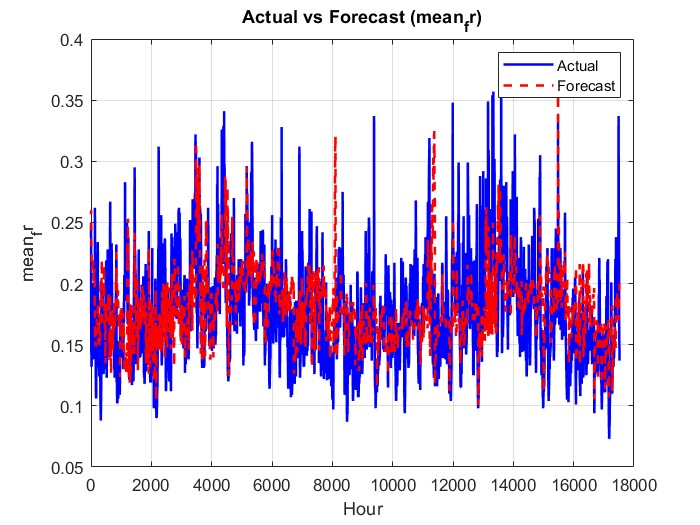
\includegraphics[width=0.5\textwidth]{graphs/hybrid/120 hours/mean_fr/actual vs forecast.jpg}\hfill
    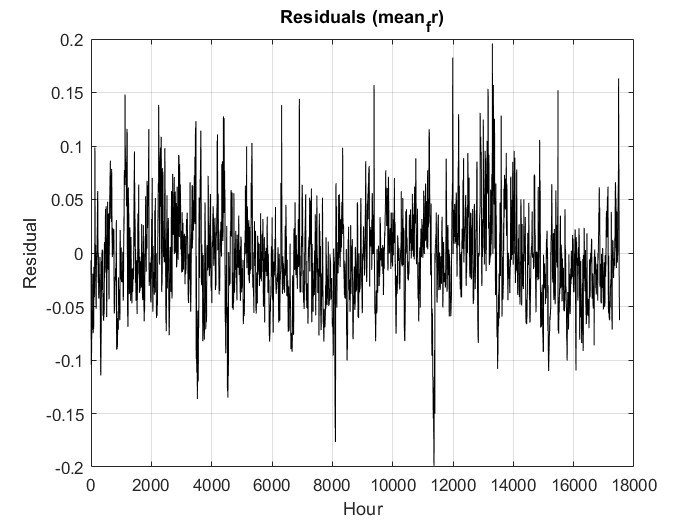
\includegraphics[width=0.5\textwidth]{graphs/hybrid/120 hours/mean_fr/residuals.jpg}\\[1ex]
    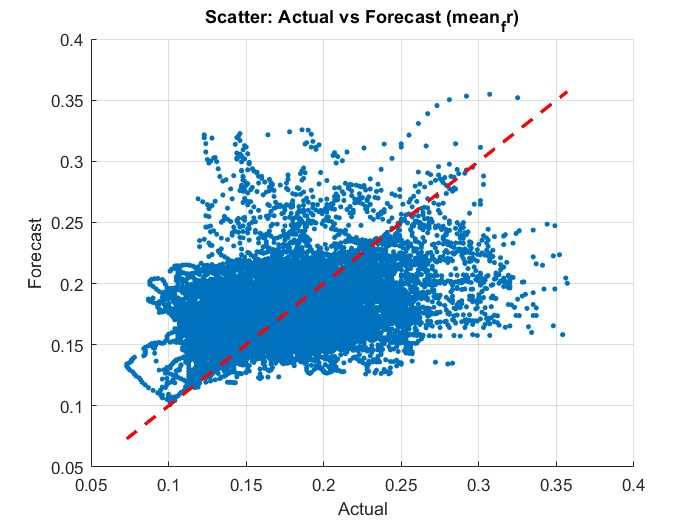
\includegraphics[width=0.5\textwidth]{graphs/hybrid/120 hours/mean_fr/scatter plot.jpg}\hfill
    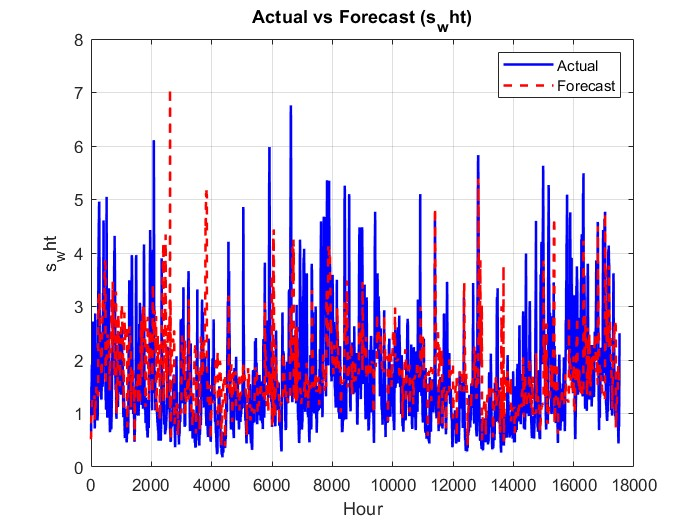
\includegraphics[width=0.5\textwidth]{graphs/hybrid/120 hours/s_wht/actual vs forecast.jpg}\\[1ex]
\end{figure}
\begin{figure}
    \centering
    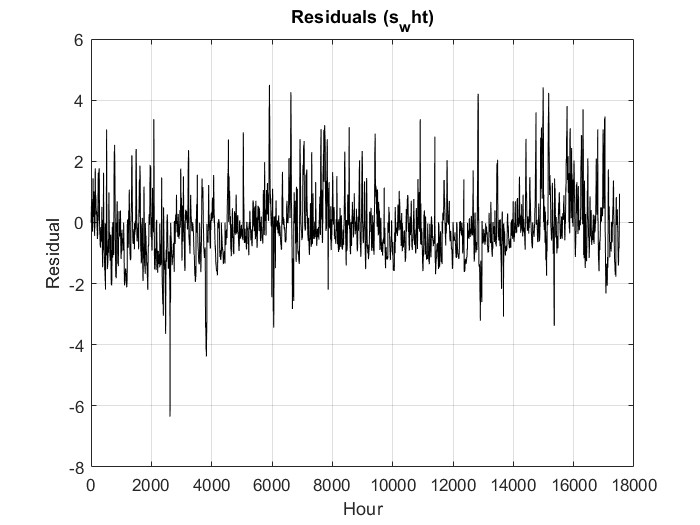
\includegraphics[width=0.5\textwidth]{graphs/hybrid/120 hours/s_wht/residuals.jpg}\hfill
    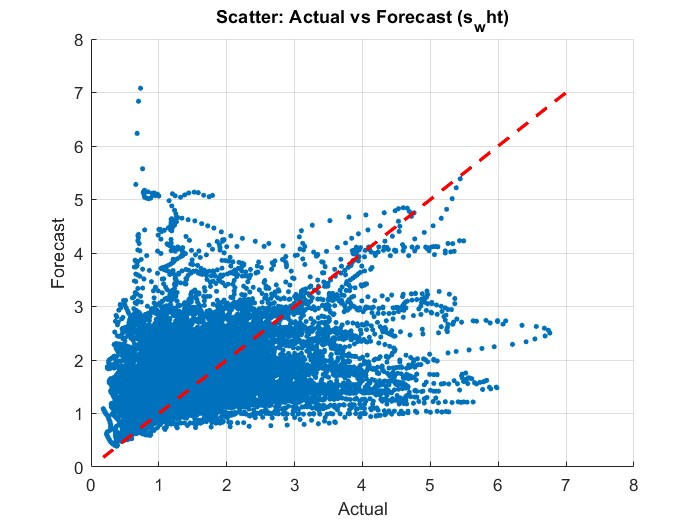
\includegraphics[width=0.5\textwidth]{graphs/hybrid/120 hours/s_wht/scatter plot.jpg}\\[1ex]
    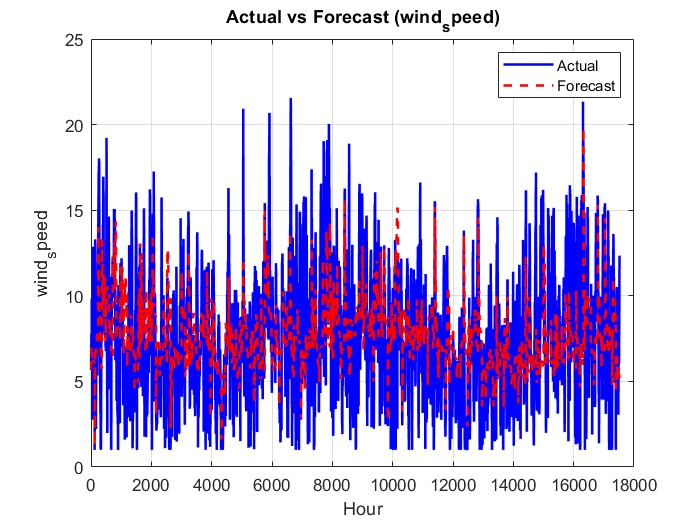
\includegraphics[width=0.5\textwidth]{graphs/hybrid/120 hours/wind speed/actual vs forecast.jpg}\hfill
    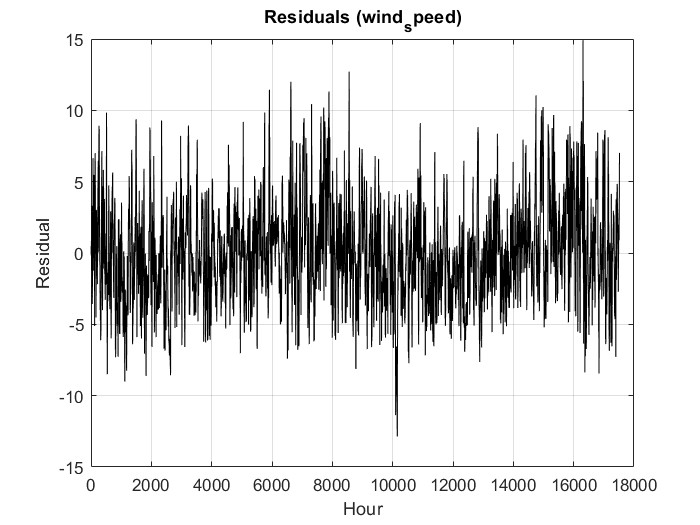
\includegraphics[width=0.5\textwidth]{graphs/hybrid/120 hours/wind speed/residuals.jpg}\\[1ex]
    \centering
    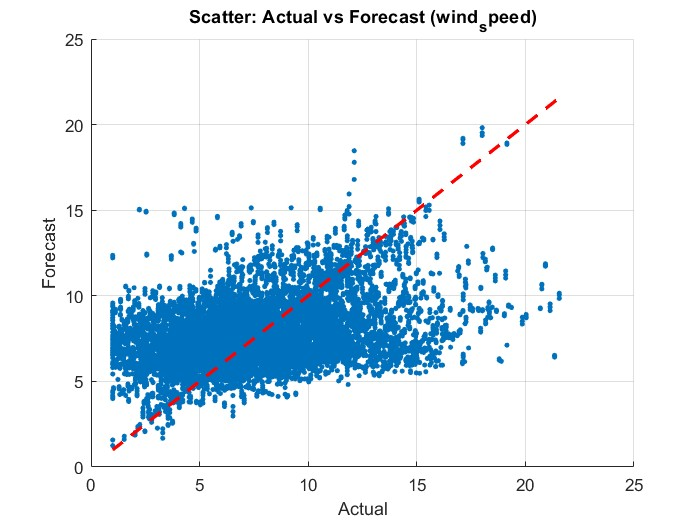
\includegraphics[width=0.5\textwidth]{graphs/hybrid/120 hours/wind speed/scatter plot.jpg}
    
    \caption{Hybrid Model Performance Visualizations for Mean Wave Frequency, Significant Wave Height, and Wind Speed.}
    \label{fig:hybrid_all}
\end{figure}

\begin{figure}[ht!]
    \centering
    \includegraphics[width=0.5\textwidth]{"graphs/bnn with mcd/mean_fr/actual vs forecast.jpg"}\hfill
    \includegraphics[width=0.5\textwidth]{"graphs/bnn with mcd/mean_fr/residuals.jpg"}\\[1ex]
    \includegraphics[width=0.5\textwidth]{"graphs/bnn with mcd/mean_fr/scatter plot.jpg"}\hfill
    \includegraphics[width=0.5\textwidth]{"graphs/bnn with mcd/s_wht/actual vs forecast.jpg"}\\[1ex]
    \includegraphics[width=0.5\textwidth]{"graphs/bnn with mcd/s_wht/residuals.jpg"}\hfill
    \includegraphics[width=0.5\textwidth]{"graphs/bnn with mcd/s_wht/scatter plot.jpg"}\\[1ex]
\end{figure}
\begin{figure}
    \includegraphics[width=0.5\textwidth]{"graphs/bnn with mcd/wind speed/actual vs forecast.jpg"}\hfill
    \includegraphics[width=0.5\textwidth]{"graphs/bnn with mcd/wind speed/residuals.jpg"}\\[1ex]
    \centering
    \includegraphics[width=0.5\textwidth]{"graphs/bnn with mcd/wind speed/scatter plot.jpg"}    
    \caption{BNN with MC dropout Model Performance Visualizations for Mean Wave Frequency, Significant Wave Height, and Wind Speed.}
    \label{fig:bnn_mcd_all}
\end{figure}

\begin{figure}[ht!]
    \centering
    \includegraphics[width=0.5\textwidth]{"graphs/lstm/mean_fr/actual vs forecast.jpg"}\hfill
    \includegraphics[width=0.5\textwidth]{"graphs/lstm/mean_fr/residuals.jpg"}\\[1ex]
    \includegraphics[width=0.5\textwidth]{"graphs/lstm/mean_fr/scatter plot.jpg"}\hfill
    \includegraphics[width=0.5\textwidth]{"graphs/lstm/s_wht/actual vs forecast.jpg"}\\[1ex]
    \includegraphics[width=0.5\textwidth]{"graphs/lstm/s_wht/residuals.jpg"}\hfill
    \includegraphics[width=0.5\textwidth]{"graphs/lstm/s_wht/scatter plot.jpg"}\\[1ex]
\end{figure}
\begin{figure}
    \includegraphics[width=0.5\textwidth]{"graphs/lstm/wind_speed/actual vs forecast.jpg"}\hfill
    \includegraphics[width=0.5\textwidth]{"graphs/lstm/wind_speed/residuals.jpg"}\\[1ex]
    \centering
    \includegraphics[width=0.5\textwidth]{"graphs/lstm/wind_speed/scatter plot.jpg"}    
    \caption{LSTM Model Performance Visualizations for Mean Wave Frequency, Significant Wave Height, and Wind Speed.}
    \label{fig:lstm_all}
\end{figure}
\chapter{Results Hybrid model multiple Refit Intervals}
\label{results hybrid different refit}

\begin{figure}[ht!]
  \centering
  \begin{tabular}{ccc}
    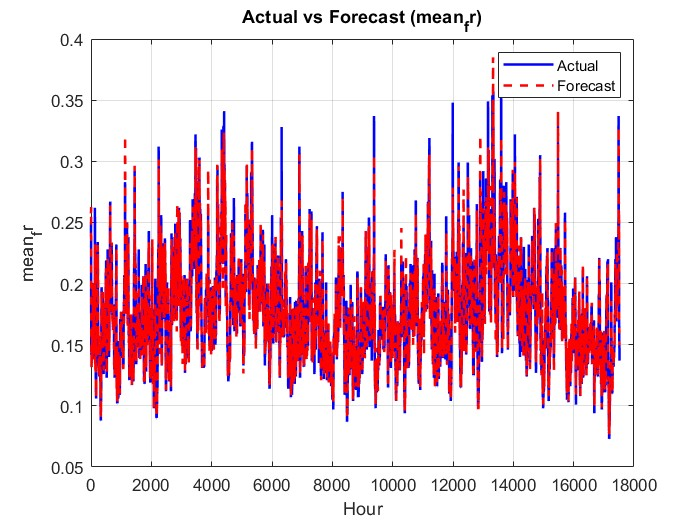
\includegraphics[width=0.32\textwidth]{graphs/hybrid/6 hours/mean_fr/actual vs forecast.jpg} &
    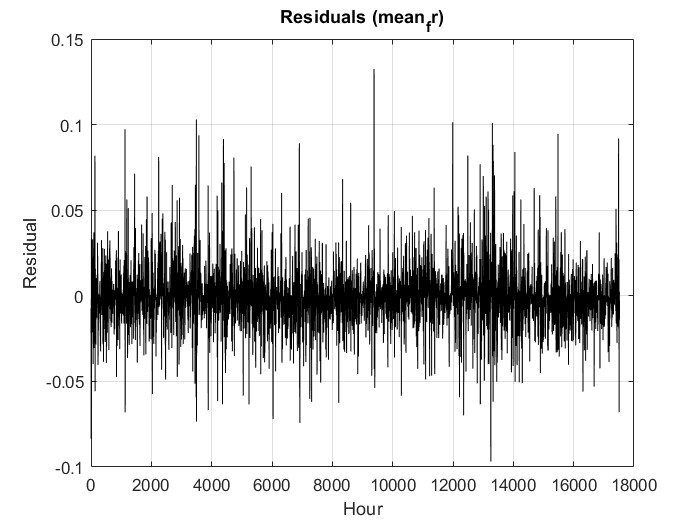
\includegraphics[width=0.32\textwidth]{graphs/hybrid/6 hours/mean_fr/residuals.jpg} &
    \includegraphics[width=0.32\textwidth]{graphs/hybrid/6 hours/mean_fr/scatter plot.jpg} \\
    \includegraphics[width=0.32\textwidth]{graphs/hybrid/6 hours/s_wht/actual vs forecast.jpg} &
    \includegraphics[width=0.32\textwidth]{graphs/hybrid/6 hours/s_wht/residuals.jpg} &
    \includegraphics[width=0.32\textwidth]{graphs/hybrid/6 hours/s_wht/scatter plot.jpg} \\
    \includegraphics[width=0.32\textwidth]{graphs/hybrid/6 hours/wind_speed/actual vs forecast.jpg} &
    \includegraphics[width=0.32\textwidth]{graphs/hybrid/6 hours/wind_speed/residuals.jpg} &
    \includegraphics[width=0.32\textwidth]{graphs/hybrid/6 hours/wind_speed/scatter plot.jpg} \\
  \end{tabular}
  \caption{Hybrid Model 6 hours Performance Visualizations for Mean Wave Frequency, Significant Wave Height, and Wind Speed.}
  \label{fig:hybrid_6_hours}
\end{figure}


\begin{figure}[ht!]
  \centering
  \begin{tabular}{ccc}
    \includegraphics[width=0.32\textwidth]{graphs/hybrid/12 hours/mean_fr/actual vs forecast.jpg} &
    \includegraphics[width=0.32\textwidth]{graphs/hybrid/12 hours/mean_fr/residuals.jpg} &
    \includegraphics[width=0.32\textwidth]{graphs/hybrid/12 hours/mean_fr/scatter plot.jpg} \\
    \includegraphics[width=0.32\textwidth]{graphs/hybrid/12 hours/s_wht/actual vs forecast.jpg} &
    \includegraphics[width=0.32\textwidth]{graphs/hybrid/12 hours/s_wht/residuals.jpg} &
    \includegraphics[width=0.32\textwidth]{graphs/hybrid/12 hours/s_wht/scatter plot.jpg} \\
    \includegraphics[width=0.32\textwidth]{graphs/hybrid/12 hours/wind_speed/actual vs forecast.jpg} &
    \includegraphics[width=0.32\textwidth]{graphs/hybrid/12 hours/wind_speed/residuals wind speed.jpg} &
    \includegraphics[width=0.32\textwidth]{graphs/hybrid/12 hours/wind_speed/scatter plot.jpg} \\
  \end{tabular}
  \caption{Hybrid Model 12 hours Performance Visualizations for Mean Wave Frequency, Significant Wave Height, and Wind Speed.}
  \label{fig:hybrid_12_hours}
\end{figure}

\begin{figure}[ht!]
  \centering
  \begin{tabular}{ccc}
    \includegraphics[width=0.32\textwidth]{graphs/hybrid/24 hours/mean_fr/actual vs forecast.jpg} &
    \includegraphics[width=0.32\textwidth]{graphs/hybrid/24 hours/mean_fr/residuals.jpg} &
    \includegraphics[width=0.32\textwidth]{graphs/hybrid/24 hours/mean_fr/scatter plot.jpg} \\
    \includegraphics[width=0.32\textwidth]{graphs/hybrid/24 hours/s_wht/actual vs forecast.jpg} &
    \includegraphics[width=0.32\textwidth]{graphs/hybrid/24 hours/s_wht/residuals.jpg} &
    \includegraphics[width=0.32\textwidth]{graphs/hybrid/24 hours/s_wht/scatter plot.jpg} \\
    \includegraphics[width=0.32\textwidth]{graphs/hybrid/24 hours/wind_speed/actual vs forecast.jpg} &
    \includegraphics[width=0.32\textwidth]{graphs/hybrid/24 hours/wind_speed/residuals.jpg} &
    \includegraphics[width=0.32\textwidth]{graphs/hybrid/24 hours/wind_speed/scatter plot.jpg} \\
  \end{tabular}
  \caption{Hybrid Model 24 hours Performance Visualizations for Mean Wave Frequency, Significant Wave Height, and Wind Speed.}
  \label{fig:hybrid_24_hours}
\end{figure}

\begin{figure}[ht!]
  \centering
  \begin{tabular}{ccc}
    \includegraphics[width=0.32\textwidth]{graphs/hybrid/36 hours/mean_fr/actual vs forecast.jpg} &
    \includegraphics[width=0.32\textwidth]{graphs/hybrid/36 hours/mean_fr/residuals.jpg} &
    \includegraphics[width=0.32\textwidth]{graphs/hybrid/36 hours/mean_fr/scatter plot.jpg} \\
    \includegraphics[width=0.32\textwidth]{graphs/hybrid/36 hours/s_wht/actual vs forecast.jpg} &
    \includegraphics[width=0.32\textwidth]{graphs/hybrid/36 hours/s_wht/residuals.jpg} &
    \includegraphics[width=0.32\textwidth]{graphs/hybrid/36 hours/s_wht/scatter plot.jpg} \\
    \includegraphics[width=0.32\textwidth]{graphs/hybrid/36 hours/wind_speed/actual vs forecast.jpg} &
    \includegraphics[width=0.32\textwidth]{graphs/hybrid/36 hours/wind_speed/residuals.jpg} &
    \includegraphics[width=0.32\textwidth]{graphs/hybrid/36 hours/wind_speed/scatter plot.jpg} \\
  \end{tabular}
  \caption{Hybrid Model 36 hours Performance Visualizations for Mean Wave Frequency, Significant Wave Height, and Wind Speed.}
  \label{fig:hybrid_36_hours}
\end{figure}

\begin{figure}[ht!]
  \centering
  \begin{tabular}{ccc}
    \includegraphics[width=0.32\textwidth]{graphs/hybrid/48 hours/mean_fr/actual vs forecast.jpg} &
    \includegraphics[width=0.32\textwidth]{graphs/hybrid/48 hours/mean_fr/residuals.jpg} &
    \includegraphics[width=0.32\textwidth]{graphs/hybrid/48 hours/mean_fr/scatter plot.jpg} \\
    \includegraphics[width=0.32\textwidth]{graphs/hybrid/48 hours/s_wht/actual vs forecast.jpg} &
    \includegraphics[width=0.32\textwidth]{graphs/hybrid/48 hours/s_wht/residuals.jpg} &
    \includegraphics[width=0.32\textwidth]{graphs/hybrid/48 hours/s_wht/scatter plot.jpg} \\
    \includegraphics[width=0.32\textwidth]{graphs/hybrid/48 hours/wind_speed/actual vs forecast.jpg} &
    \includegraphics[width=0.32\textwidth]{graphs/hybrid/48 hours/wind_speed/residuals.jpg} &
    \includegraphics[width=0.32\textwidth]{graphs/hybrid/48 hours/wind_speed/scatter plot.jpg} \\
  \end{tabular}
  \caption{Hybrid Model 48 hours Performance Visualizations for Mean Wave Frequency, Significant Wave Height, and Wind Speed.}
  \label{fig:hybrid_48_hours}
\end{figure}

\begin{figure}[ht!]
  \centering
  \begin{tabular}{ccc}
    \includegraphics[width=0.32\textwidth]{graphs/hybrid/72 hours/mean_fr/actual vs forecast.jpg} &
    \includegraphics[width=0.32\textwidth]{graphs/hybrid/72 hours/mean_fr/residuals.jpg} &
    \includegraphics[width=0.32\textwidth]{graphs/hybrid/72 hours/mean_fr/scatter plot.jpg} \\
    \includegraphics[width=0.32\textwidth]{graphs/hybrid/72 hours/s_wht/actual vs forecast.jpg} &
    \includegraphics[width=0.32\textwidth]{graphs/hybrid/72 hours/s_wht/residuals.jpg} &
    \includegraphics[width=0.32\textwidth]{graphs/hybrid/72 hours/s_wht/scatter plot.jpg} \\
    \includegraphics[width=0.32\textwidth]{graphs/hybrid/72 hours/wind_speed/actual vs forecast.jpg} &
    \includegraphics[width=0.32\textwidth]{graphs/hybrid/72 hours/wind_speed/residuals.jpg} &
    \includegraphics[width=0.32\textwidth]{graphs/hybrid/72 hours/wind_speed/scatter plot.jpg} \\
  \end{tabular}
  \caption{Hybrid Model 72 hours Performance Visualizations for Mean Wave Frequency, Significant Wave Height, and Wind Speed.}
  \label{fig:hybrid_72_hours}
\end{figure}

\begin{figure}[ht!]
  \centering
  \begin{tabular}{ccc}
    \includegraphics[width=0.32\textwidth]{graphs/hybrid/96 hours/mean_fr/actual vs forecast.jpg} &
    \includegraphics[width=0.32\textwidth]{graphs/hybrid/96 hours/mean_fr/residuals.jpg} &
    \includegraphics[width=0.32\textwidth]{graphs/hybrid/96 hours/mean_fr/scatter plot.jpg} \\
    \includegraphics[width=0.32\textwidth]{graphs/hybrid/96 hours/s_wht/actual vs forecast.jpg} &
    \includegraphics[width=0.32\textwidth]{graphs/hybrid/96 hours/s_wht/residuals.jpg} &
    \includegraphics[width=0.32\textwidth]{graphs/hybrid/96 hours/s_wht/scatter plot.jpg} \\
    \includegraphics[width=0.32\textwidth]{graphs/hybrid/96 hours/wind_speed/actual vs forecast.jpg} &
    \includegraphics[width=0.32\textwidth]{graphs/hybrid/96 hours/wind_speed/residuals.jpg} &
    \includegraphics[width=0.32\textwidth]{graphs/hybrid/96 hours/wind_speed/scatter plot.jpg} \\
  \end{tabular}
  \caption{Hybrid Model 96 hours Performance Visualizations for Mean Wave Frequency, Significant Wave Height, and Wind Speed.}
  \label{fig:hybrid_96_hours}
\end{figure}

\begin{figure}[ht!]
  \centering
  \begin{tabular}{ccc}
    \includegraphics[width=0.32\textwidth]{graphs/hybrid/120 hours/mean_fr/actual vs forecast.jpg} &
    \includegraphics[width=0.32\textwidth]{graphs/hybrid/120 hours/mean_fr/residuals.jpg} &
    \includegraphics[width=0.32\textwidth]{graphs/hybrid/120 hours/mean_fr/scatter plot.jpg} \\
    \includegraphics[width=0.32\textwidth]{graphs/hybrid/120 hours/s_wht/actual vs forecast.jpg} &
    \includegraphics[width=0.32\textwidth]{graphs/hybrid/120 hours/s_wht/residuals.jpg} &
    \includegraphics[width=0.32\textwidth]{graphs/hybrid/120 hours/s_wht/scatter plot.jpg} \\
    \includegraphics[width=0.32\textwidth]{graphs/hybrid/120 hours/wind speed/actual vs forecast.jpg} &
    \includegraphics[width=0.32\textwidth]{graphs/hybrid/120 hours/wind speed/residuals.jpg} &
    \includegraphics[width=0.32\textwidth]{graphs/hybrid/120 hours/wind speed/scatter plot.jpg} \\
  \end{tabular}
  \caption{Hybrid Model 120 hours Performance Visualizations for Mean Wave Frequency, Significant Wave Height, and Wind Speed.}
  \label{fig:hybrid_120_hours}
\end{figure}

\begin{figure}[ht!]
  \centering
  \begin{tabular}{ccc}
    \includegraphics[width=0.32\textwidth]{graphs/hybrid/144 hours/mean_fr/actual vs forecast.jpg} &
    \includegraphics[width=0.32\textwidth]{graphs/hybrid/144 hours/mean_fr/residuals.jpg} &
    \includegraphics[width=0.32\textwidth]{graphs/hybrid/144 hours/mean_fr/scatter plot.jpg} \\
    \includegraphics[width=0.32\textwidth]{graphs/hybrid/144 hours/s_wht/actual vs forecast.jpg} &
    \includegraphics[width=0.32\textwidth]{graphs/hybrid/144 hours/s_wht/residuals.jpg} &
    \includegraphics[width=0.32\textwidth]{graphs/hybrid/144 hours/s_wht/scatter plot.jpg} \\
    \includegraphics[width=0.32\textwidth]{graphs/hybrid/144 hours/wind_speed/actual vs forecast.jpg} &
    \includegraphics[width=0.32\textwidth]{graphs/hybrid/144 hours/wind_speed/residuals.jpg} &
    \includegraphics[width=0.32\textwidth]{graphs/hybrid/144 hours/wind_speed/scatter plot.jpg} \\
  \end{tabular}
  \caption{Hybrid Model 144 hours Performance Visualizations for Mean Wave Frequency, Significant Wave Height, and Wind Speed.}
  \label{fig:hybrid_144_hours}
\end{figure}

\begin{figure}[ht!]
  \centering
  \begin{tabular}{ccc}
    \includegraphics[width=0.32\textwidth]{graphs/hybrid/168 hours/mean_fr/actual vs forecast.jpg} &
    \includegraphics[width=0.32\textwidth]{graphs/hybrid/168 hours/mean_fr/residuals.jpg} &
    \includegraphics[width=0.32\textwidth]{graphs/hybrid/168 hours/mean_fr/scatter plot.jpg} \\
    \includegraphics[width=0.32\textwidth]{graphs/hybrid/168 hours/s_wht/actual vs forecast.jpg} &
    \includegraphics[width=0.32\textwidth]{graphs/hybrid/168 hours/s_wht/residuals.jpg} &
    \includegraphics[width=0.32\textwidth]{graphs/hybrid/168 hours/s_wht/scatter plot.jpg} \\
    \includegraphics[width=0.32\textwidth]{graphs/hybrid/168 hours/wind_speed/actual vs forecast.jpg} &
    \includegraphics[width=0.32\textwidth]{graphs/hybrid/168 hours/wind_speed/residuals.jpg} &
    \includegraphics[width=0.32\textwidth]{graphs/hybrid/168 hours/wind_speed/scatter plot.jpg} \\
  \end{tabular}
  \caption{Hybrid Model 168 hours Performance Visualizations for Mean Wave Frequency, Significant Wave Height, and Wind Speed.}
  \label{fig:hybrid_168_hours}
\end{figure}

\begin{figure}[ht!]
  \centering
  \begin{tabular}{ccc}
    \includegraphics[width=0.32\textwidth]{graphs/hybrid/336 hours/mean_fr/actual vs forecast.jpg} &
    \includegraphics[width=0.32\textwidth]{graphs/hybrid/336 hours/mean_fr/residuals.jpg} &
    \includegraphics[width=0.32\textwidth]{graphs/hybrid/336 hours/mean_fr/scatter plot.jpg} \\
    \includegraphics[width=0.32\textwidth]{graphs/hybrid/336 hours/s_wht/actual vs forecast.jpg} &
    \includegraphics[width=0.32\textwidth]{graphs/hybrid/336 hours/s_wht/residuals.jpg} &
    \includegraphics[width=0.32\textwidth]{graphs/hybrid/336 hours/s_wht/scatter plot.jpg} \\
    \includegraphics[width=0.32\textwidth]{graphs/hybrid/336 hours/wind_speed/actual vs forecast.jpg} &
    \includegraphics[width=0.32\textwidth]{graphs/hybrid/336 hours/wind_speed/residuals.jpg} &
    \includegraphics[width=0.32\textwidth]{graphs/hybrid/336 hours/wind_speed/scatter plot.jpg} \\
  \end{tabular}
  \caption{Hybrid Model 336 hours Performance Visualizations for Mean Wave Frequency, Significant Wave Height, and Wind Speed.}
  \label{fig:hybrid_336_hours}
\end{figure}

\begin{figure}[ht!]
  \centering
  \begin{tabular}{ccc}
    \includegraphics[width=0.32\textwidth]{graphs/hybrid/672 hours/mean_fr/actual vs forecast.jpg} &
    \includegraphics[width=0.32\textwidth]{graphs/hybrid/672 hours/mean_fr/residuals.jpg} &
    \includegraphics[width=0.32\textwidth]{graphs/hybrid/672 hours/mean_fr/scatter plot.jpg} \\
    \includegraphics[width=0.32\textwidth]{graphs/hybrid/672 hours/s_wht/actual vs forecast.jpg} &
    \includegraphics[width=0.32\textwidth]{graphs/hybrid/672 hours/s_wht/residuals.jpg} &
    \includegraphics[width=0.32\textwidth]{graphs/hybrid/672 hours/s_wht/scatter plot.jpg} \\
    \includegraphics[width=0.32\textwidth]{graphs/hybrid/672 hours/wind_speed/actual vs forecast.jpg} &
    \includegraphics[width=0.32\textwidth]{graphs/hybrid/672 hours/wind_speed/residuals.jpg} &
    \includegraphics[width=0.32\textwidth]{graphs/hybrid/672 hours/wind_speed/scatter plot.jpg} \\
  \end{tabular}
  \caption{Hybrid Model 672 hours Performance Visualizations for Mean Wave Frequency, Significant Wave Height, and Wind Speed.}
  \label{fig:hybrid_672_hours}
\end{figure}

\printbibliography

\end{document}

